% Options for packages loaded elsewhere
\PassOptionsToPackage{unicode}{hyperref}
\PassOptionsToPackage{hyphens}{url}
%
\documentclass[
  a4paper,
]{scrbook}

\usepackage{amsmath,amssymb}
\usepackage{iftex}
\ifPDFTeX
  \usepackage[T1]{fontenc}
  \usepackage[utf8]{inputenc}
  \usepackage{textcomp} % provide euro and other symbols
\else % if luatex or xetex
  \usepackage{unicode-math}
  \defaultfontfeatures{Scale=MatchLowercase}
  \defaultfontfeatures[\rmfamily]{Ligatures=TeX,Scale=1}
\fi
\usepackage{lmodern}
\ifPDFTeX\else  
    % xetex/luatex font selection
  \setmainfont[]{Latin Modern Roman}
  \setsansfont[]{Latin Modern Roman}
\fi
% Use upquote if available, for straight quotes in verbatim environments
\IfFileExists{upquote.sty}{\usepackage{upquote}}{}
\IfFileExists{microtype.sty}{% use microtype if available
  \usepackage[]{microtype}
  \UseMicrotypeSet[protrusion]{basicmath} % disable protrusion for tt fonts
}{}
\makeatletter
\@ifundefined{KOMAClassName}{% if non-KOMA class
  \IfFileExists{parskip.sty}{%
    \usepackage{parskip}
  }{% else
    \setlength{\parindent}{0pt}
    \setlength{\parskip}{6pt plus 2pt minus 1pt}}
}{% if KOMA class
  \KOMAoptions{parskip=half}}
\makeatother
\usepackage{xcolor}
\setlength{\emergencystretch}{3em} % prevent overfull lines
\setcounter{secnumdepth}{5}
% Make \paragraph and \subparagraph free-standing
\ifx\paragraph\undefined\else
  \let\oldparagraph\paragraph
  \renewcommand{\paragraph}[1]{\oldparagraph{#1}\mbox{}}
\fi
\ifx\subparagraph\undefined\else
  \let\oldsubparagraph\subparagraph
  \renewcommand{\subparagraph}[1]{\oldsubparagraph{#1}\mbox{}}
\fi


\providecommand{\tightlist}{%
  \setlength{\itemsep}{0pt}\setlength{\parskip}{0pt}}\usepackage{longtable,booktabs,array}
\usepackage{calc} % for calculating minipage widths
% Correct order of tables after \paragraph or \subparagraph
\usepackage{etoolbox}
\makeatletter
\patchcmd\longtable{\par}{\if@noskipsec\mbox{}\fi\par}{}{}
\makeatother
% Allow footnotes in longtable head/foot
\IfFileExists{footnotehyper.sty}{\usepackage{footnotehyper}}{\usepackage{footnote}}
\makesavenoteenv{longtable}
\usepackage{graphicx}
\makeatletter
\def\maxwidth{\ifdim\Gin@nat@width>\linewidth\linewidth\else\Gin@nat@width\fi}
\def\maxheight{\ifdim\Gin@nat@height>\textheight\textheight\else\Gin@nat@height\fi}
\makeatother
% Scale images if necessary, so that they will not overflow the page
% margins by default, and it is still possible to overwrite the defaults
% using explicit options in \includegraphics[width, height, ...]{}
\setkeys{Gin}{width=\maxwidth,height=\maxheight,keepaspectratio}
% Set default figure placement to htbp
\makeatletter
\def\fps@figure{htbp}
\makeatother

\usepackage{booktabs}
\usepackage{longtable}
\usepackage{array}
\usepackage{multirow}
\usepackage{wrapfig}
\usepackage{float}
\usepackage{colortbl}
\usepackage{pdflscape}
\usepackage{tabu}
\usepackage{threeparttable}
\usepackage{threeparttablex}
\usepackage[normalem]{ulem}
\usepackage{makecell}
\usepackage{xcolor}
\usepackage{fancyhdr}
\usepackage{titling}
\setlength{\droptitle}{-2cm}
\preauthor{
  \begin{center}
  \Large
  \vspace{10mm}
  by
  \vspace{20mm}
}
\postauthor{
  \end{center}
  \vfill
}

\predate{
  \begin{center}
  A thesis 
  submitted in partial fulfilment of the \\
  requirements of the degree of \\
  Doctor of Philosophy in Physics\\               % Degree
  School of Physical and Chemical Sciences\\          % Department
  Te Herenga Waka - Victoria University of Wellington\\                       % University 
  \vspace{5mm}
}
\postdate{
  \\
  
\includegraphics[width=3in,height=1.5in]{figures/VUW-logo.png}\\
  \end{center}
  }

\renewcommand{\topfraction}{.8}
\renewcommand{\bottomfraction}{.7}
\renewcommand{\textfraction}{.15}
\renewcommand{\floatpagefraction}{.8}
\setcounter{topnumber}{3}
\setcounter{bottomnumber}{3}
\setcounter{totalnumber}{4}

\clubpenalty=9996
\widowpenalty=9999
\makeatletter
\makeatother
\makeatletter
\@ifpackageloaded{bookmark}{}{\usepackage{bookmark}}
\makeatother
\makeatletter
\@ifpackageloaded{caption}{}{\usepackage{caption}}
\AtBeginDocument{%
\ifdefined\contentsname
  \renewcommand*\contentsname{Table of contents}
\else
  \newcommand\contentsname{Table of contents}
\fi
\ifdefined\listfigurename
  \renewcommand*\listfigurename{List of Figures}
\else
  \newcommand\listfigurename{List of Figures}
\fi
\ifdefined\listtablename
  \renewcommand*\listtablename{List of Tables}
\else
  \newcommand\listtablename{List of Tables}
\fi
\ifdefined\figurename
  \renewcommand*\figurename{Figure}
\else
  \newcommand\figurename{Figure}
\fi
\ifdefined\tablename
  \renewcommand*\tablename{Table}
\else
  \newcommand\tablename{Table}
\fi
}
\@ifpackageloaded{float}{}{\usepackage{float}}
\floatstyle{ruled}
\@ifundefined{c@chapter}{\newfloat{codelisting}{h}{lop}}{\newfloat{codelisting}{h}{lop}[chapter]}
\floatname{codelisting}{Listing}
\newcommand*\listoflistings{\listof{codelisting}{List of Listings}}
\makeatother
\makeatletter
\@ifpackageloaded{caption}{}{\usepackage{caption}}
\@ifpackageloaded{subcaption}{}{\usepackage{subcaption}}
\makeatother
\makeatletter
\@ifpackageloaded{tcolorbox}{}{\usepackage[skins,breakable]{tcolorbox}}
\makeatother
\makeatletter
\@ifundefined{shadecolor}{\definecolor{shadecolor}{rgb}{.97, .97, .97}}
\makeatother
\makeatletter
\makeatother
\makeatletter
\makeatother
\ifLuaTeX
  \usepackage{selnolig}  % disable illegal ligatures
\fi
\usepackage[citestyle = ieee,urldate = iso8601]{biblatex}
\addbibresource{references.bib}
\IfFileExists{bookmark.sty}{\usepackage{bookmark}}{\usepackage{hyperref}}
\IfFileExists{xurl.sty}{\usepackage{xurl}}{} % add URL line breaks if available
\urlstyle{same} % disable monospaced font for URLs
\hypersetup{
  pdftitle={Developing an Insect Odorant Receptor Bioelectronic Nose for Vapour-Phase Detection},
  pdfauthor={Eddyn Oswald Perkins Treacher},
  hidelinks,
  pdfcreator={LaTeX via pandoc}}

\title{Developing an Insect Odorant Receptor Bioelectronic Nose for
Vapour-Phase Detection}
\author{Eddyn Oswald Perkins Treacher}
\date{Nov 2024}

\begin{document}
\frontmatter

\maketitle

\clearpage
\newpage
\thispagestyle{empty} % Hide header and footer on this page
\mbox{~}
\clearpage
\newpage

%----------------------------------------------
%   Abstract
%----------------------------------------------

\thispagestyle{plain}

\begin{flushleft}
% Manually add a section to the table of contents
\pagenumbering{roman}
\addcontentsline{toc}{chapter}{Abstract}
\huge\textbf{Abstract}
\end{flushleft}

\vspace*{\baselineskip}

The ability to detect volatile organic compounds in a highly sensitive and selective manner is desirable for applications as varied as diagnosis of illnesses at a remote clinic, monitoring of air in an industrial setting, or identification of invasive organisms at a biosecurity checkpoint. Historically, animal noses have been used for such tasks, as their combined sensitivity and selectivity are superior to traditional artificial sensors. However, training and deploying animals in such situations is both time and cost intensive. In recent years, an improved understanding of \textit{in vivo} biological sensing has driven efforts to mimic these highly efficient processes in an artificial sensor format. \\[5pt] To this end, a “bioelectronic nose” was developed. This sensor uses an artificial transducer to amplify responses of an insect odorant receptor protein to specific volatile compounds. Thin-film transistors were used as the amplifier element, given their low cost, small size and extreme sensitivity. Various thin-film morphologies were compared, and their suitability for bioelectronic nose development assessed. Transducers made using a novel steam-assisted thin-film deposition technique were found to have highly consistent device-to-device electrical properties relative to other films. Films made using this process typically showed more surface contamination than other morphologies, but their high sensitivity was nonetheless confirmed with a non-specific sensing series in an aqueous environment. \\[5pt] One of the major challenges encountered in this thesis was variability in the quality of sensor functionalisation. Raman spectroscopy and fluorescence microscopy confirmed an existing non-covalent attachment method could successfully immobilise nanodiscs onto the transistor channel region. However, various sensors functionalised using the same procedure often exhibited no sensing activity. Extensive electrical characterisation indicated the presence of an unidentified contamination layer preventing electrical interaction between the insect odorant receptors and transducer thin-film. It was shown that this layer was unlikely to be directly associated with the thin-film morphology used for the transducer. \\[5pt] Subsequently, an alternative biotin-based non-covalent method was used for functionalisation of the proteins, which eliminated several possible contamination sources. This alternative biotin-based method was used to demonstrate successful aqueous sensing of femtomolar concentrations of methyl salicylate by an iOR10a-functionalised device. When tested in a custom-built vapour delivery system, a similar bioelectronic sensor was shown to be highly sensitive to the target vapour. However, consistent reproduction of the biotin-based method was challenging due to the harsh cleaning method involved. It was therefore difficult to determine conclusively whether sensor responses were selective. By finding new, systematic approaches to address the major barriers to sensor success carefully identified in this work, there are promising signs that a highly reliable vapour-phase bioelectronic nose can be produced.

%\fancyhf{} %clear all headers and footers fields
%\thispagestyle{fancy} % Change header and footer on this page
%\renewcommand{\headrulewidth}{0pt}
%\fancyhead[L]{\textit{Abstract}} % Set header content
%\fancyfoot[L]{\thepage} %prints the page number on the right side of the header

\clearpage
\newpage
\thispagestyle{empty} % Hide header and footer on this page
\mbox{~}
\clearpage
\newpage


%----------------------------------------------
%   Acknowledgement
%----------------------------------------------

\thispagestyle{plain}

\begin{flushleft}
% Manually add a section to the table of contents
\addcontentsline{toc}{chapter}{Acknowledgements}
\huge\textbf{Acknowledgements}
\end{flushleft}

\vspace*{\baselineskip}

I would first like to acknowledge the lands of my ancestors, and the lands of the sovereign first peoples to which my ancestors travelled. We each come from the land, live off the land and return to the land.\\[5pt]
\textit{Noon of Essex to Warrang, on the Friends, Autumn 1811} \\[5pt]
\textit{Cave of Cambridgeshire to Warrang, on the Royal Charlotte, Autumn 1825} \\[5pt]
\textit{Boyce of Suffolk to Warrang, 1832} \\[5pt] 
\textit{Charlton of Northumberland to Warrang, on the Clyde, Spring 1834} \\[5pt]
\textit{Prouse of Devonshire to Pito-one, on the Duke of Roxburgh, Summer 1840} \\[5pt]
\textit{Ebden of Devonshire to Pito-one, on the Tyne, Winter 1841} \\[5pt]
\textit{Collis of Hampshire to Pito-one, on the Birman, Autumn 1842} \\[5pt]
\textit{Swann of Loch Garman to Te Whanganui-a-Tara, 1844} \\[5pt] 
\textit{Blythe of Berkshire to Whakatū, circa 1846} \\[5pt]
\textit{Innes of Berkshire to Naarm, on the Sacramento, Autumn 1853} \\[5pt]
\textit{Sheppard of Gloucestershire to Naarm, 1853} \\[5pt] 
\textit{Bruce of London to Naarm, on the Omega, Autumn 1855} \\[5pt]
\textit{Quennell of Surrey to Warrang, on the Asiatic, Winter 1855} \\[5pt]
\textit{Barr of Glasgow to Kōpūtai, on the Sir Edward Paget, Winter 1856} \\[5pt] 
\textit{Perkins of London to Te Whanganui-a-Tara, on the Matoaka, Spring 1859} \\[5pt]
\textit{McKee of Antrim to Tāmaki Makaurau, on the Indian Empire, Spring 1862} \\[5pt]
\textit{Sandilands of Peeblesshire to Ōtepoti, circa 1864} \\[5pt] 
\textit{Treacher of Berkshire to Te Whanganui-a-Tara, on the Wild Duck, Summer 1865} \\[5pt]
\textit{McTaggart of Argyllshire to Kōpūtai, on the Edward P. Bouverie, Autumn 1869} \\[5pt] 
\textit{Chapman of Kent to Whakatū, on the Adamant, Winter 1874} \\[5pt]
\textit{Cheel of London to Whakatū, on the Queen Bee, Winter 1877} \\[5pt]  
\textit{Hutchison of Aberdeen to Tarntanya, before 1882.} \\[5pt] 
I chose to start my doctoral studies just a few months into a global pandemic. Completing a challenging project with a worldwide crisis in the background might have been impossible without the supervision of AProf. Natalie Plank. Her ability to adapt to and overcome any problem has taught me that there is no situation which is truly unmanageable. I am deeply grateful for her leadership throughout a time of particular chaos. \newpage
\fancyhf{} %clear all headers and footers fields
\thispagestyle{fancy} % Change header and footer on this page
\renewcommand{\headrulewidth}{0pt}
\fancyhead[L]{\textit{Acknowledgements}} % Set header content
\fancyfoot[L]{\thepage} %prints the page number on the left side of the header 
I started this project with minimal formal training in biological science, coming from a primarily physics and engineering background. \\[5pt] The immense support I received from Melissa Jordan and Colm Carraher from the Institute for Plant and Food Research (PFR) to complete this project meant that this was not an issue, and I thank them both immensely for this. \\[5pt] I would not have been able to begin this thesis without the financial backing and support I received from PFR and the Better Border Biosecurity (B3) programme. In particular, I am very grateful to Andrew Kralicek, formerly with PFR and now at Scentian Bio, and the ex-Director of B3, David Teulon, for helping to secure funding for my project. I would also like to thank the donor of the Ernest Marsden Scholarship in Physics for their significant financial support. \\[5pt] There are many incredibly supportive people who I worked alongside during my project. I would like to start off by thanking Rifat Ullah, whose mentoring and kindness encouraged me to pursue further study. His work on the initial design and setup of the vapour delivery system was invaluable to me throughout this project. I am also especially grateful to Alex Puglisi, for constructing the mechanical elements of the vapour delivery system and giving me extensive feedback on the system design. I would like to thank Peter Coard, for his advice and guidance when constructing the electrical elements of the vapour delivery system. I thank Selvan Murugathas, too, for his advice on constructing the insect odorant receptor sensors, as well as Damon Colbert and Valentina Lucarelli, who provided the insect odorant receptor nanodiscs used in this work. \\[5pt] Thank you to AProf. Ben Ruck, my supportive secondary supervisor, and to AProf. Franck Natali, for always asking about my thesis in the tearoom. Thank you to Gideon Gouws for his friendly encouragement and advice. For their substantial technical assistance and mentoring during this project, I thank Alan Rennie, Grant Franklin, Chris Lepper, Rashika Gunasekara, Pete Jebson and Sushila Pillai from VUW, Andrew Chan from PFR, AProf. Charles Unsworth from the University of Auckland, and Prof. Simon Brown and his nanomaterials group from the University of Canterbury. \\[5pt] I was lucky enough to start my doctoral program just as a group of supportive and talented senior students were finishing, and finished just as a group of enthusiastic and talented new doctoral students were starting. A special thanks to Jenna Nyugen, Erica Happe and Erica Cassie for teaching me the fabrication processes and characterisation procedures that made this thesis happen; and a special thanks to Marissa Dierkes, Danica Fontein, Sangar Begzaad and Alireza Zare, for their incredible support throughout the thesis writing process. I am also thankful for the assistance of the cleanroom group interns over the course of my PhD, including Liam, Hayden and Lotte. I would further like to thank everyone else I shared an office with and worked alongside, including Jackson, Will, Roshni, Ali, Kira, Catherine, Martin, Janani, Ted, Kiri and Joe. \\[5pt] A massive thank you to Openstar Technologies. It has been an honour to work on a cutting-edge plasma physics project right here in Te Whanganui-a-Tara. A particularly big thank you to Ratu, Darren, Thomas and Craig for having me as part of the plasma physics team. Thank you also to the other Openstar interns, in particular the other plasma physics interns, Valentina, Benjy and Chris. I wish you success in all your dipole-confined plasma related endeavours. \\[5pt] I want to thank Shodokan Aikido New Zealand for their support throughout this thesis, in particular for the once-in-a-lifetime opportunity to travel to Osaka to be graded for first-dan by Nariyama Shihan. Thanks for all the training and support, Ian. Thank you to all the friends and family, old and new, who have supported me over these wild past few years. You know who you are. \\[5pt] Thank you to my brother, Keeson, and to my parents, Hilary and Phillip. Your support means everything to me, and I would not be where I am today without you. Our Friday lunchtime cafe visits inspired and motivated me throughout the doctoral program. Thank you, thank you, thank you for your love, your compassion, and for being there for me. \\[5pt] Finally, thank you Nina. Your love has kept me going through the most difficult and most wonderful times over the last three and a half years. You are the light of my life, and I am so happy to have taken on this challenge with you by my side. \\[5pt] Arohanui and peace to you all, Eddyn (Ned)

\fancyhf{} %clear all headers and footers fields
\thispagestyle{fancy} % Change header and footer on this page
\renewcommand{\headrulewidth}{0pt}
\fancyhead[R]{\textit{Acknowledgements}} % Set header content
\fancyfoot[R]{\thepage} %prints the page number on the right side of the header

\clearpage
\newpage
\thispagestyle{empty} % Hide header and footer on this page
\mbox{~}
\clearpage
\newpage

\pagestyle{headings}

\ifdefined\Shaded\renewenvironment{Shaded}{\begin{tcolorbox}[interior hidden, borderline west={3pt}{0pt}{shadecolor}, frame hidden, enhanced, breakable, boxrule=0pt, sharp corners]}{\end{tcolorbox}}\fi

\renewcommand*\contentsname{Table of Contents}
{
\setcounter{tocdepth}{2}
\addcontentsline{toc}{chapter}{Table of Contents}
\tableofcontents
}
\listoffigures
\addcontentsline{toc}{chapter}{List of Figures}
\listoftables
\addcontentsline{toc}{chapter}{List of Tables}

\clearpage
\newpage
\thispagestyle{empty} % Hide header and footer on this page
\mbox{~}
\clearpage
\newpage

%----------------------------------------------
%   List of Abbreviations
%----------------------------------------------

\thispagestyle{plain}

\begin{flushleft}
% Manually add a section to the table of contents
\addcontentsline{toc}{chapter}{List of Abbreviations}
\huge\textbf{List of Abbreviations}
\end{flushleft}

\vspace*{\baselineskip}

\begin{table}[H]
  \begin{tabular}{@{}p{0.25\textwidth} p{0.75\textwidth}@{}}  % Adjust the width as needed
    2D  & 2-Dimensional  \\[5pt]
    Ab  & Antibody  \\[5pt]
    AB  & Amyl Butyrate  \\[5pt]
    AB-NTA  & N$\alpha$,N$\alpha$-Bis(carboxymethyl)-\textit{L}-lysine hydrate  \\[5pt]
    AFM  & Atomic Force Microscope/Microscopy  \\[5pt]
    AH  & Absolute Humidity  \\[5pt]
    Avi-tag  & Avidin-tag  \\[5pt]
    BMIM  & 1-butyl-3-methylimidazolium bis(trifluoromethylsulfonyl)imide  \\[5pt]
    BWF  & Breit-Wigner-Fano  \\[5pt]
    CAD  & Computer Aided Design \\[5pt]
    CNT  & Carbon Nanotube  \\[5pt]
    CVD  & Chemical Vapour Deposition  \\[5pt]
    Cy3  & Cyanine 3  \\[5pt]
    DAN  & 1,5-diaminonaphthalene  \\[5pt]
    DAQ  & Data Acquisition Input/Output Module  \\[5pt]
    DCB  & 1,2-dichlorobenzene  \\[5pt]
    DI  & Deionised  \\[5pt]
    DMF  & Dimethylformamide   \\[5pt]
    DMSO  & Dimethylsulfoxide   \\[5pt]
    DMT-MM   & 4-(4,6-dimethoxy-1,3,5-triazin-2-yl)-4 methylmorpholinium chloride \\[5pt]
    DMMP  & Dimethyl Methylphosphonate  \\[5pt]
    DNA  & Deoxyribonucleic Acid  \\[5pt]
    E2Hex  & \textit{trans}-2-hexan-1-al  \\[5pt]
    EB  & Ethyl Butyrate  \\[5pt]
    EDC  & 1-Ethyl-3-(3-dimethylaminopropyl)carbodiimide  \\[5pt]
    EDL  & Electric Double Layer  \\[5pt]
    EIS  & Electrochemical Impedance Spectroscopy  \\[5pt]
    EtHex  & Ethyl Hexanoate  \\[5pt]
    EtOH  & Ethanol  \\[5pt]
  \end{tabular}
\end{table}

\newpage
\fancyhf{} %clear all headers and footers fields
\thispagestyle{fancy} % Change header and footer on this page
\renewcommand{\headrulewidth}{0pt}
\fancyhead[L]{\textit{List of Abbreviations}} % Set header content
\fancyfoot[L]{\thepage} %prints the page number on the right side of the header
\begin{table}[H]
  \begin{tabular}{@{}p{0.25\textwidth} p{0.75\textwidth}@{}}  % Adjust the width as needed
    FET  & Field-Effect Transistor  \\[5pt]
    FITC  & Fluorescein isothiocyanate  \\[5pt]
    GA  & Glutaraldehyde  \\[5pt]
    GFET  & Graphene Field-Effect Transistor  \\[5pt]
    GFP  & Green Fluorescent Protein  \\[5pt]
    GPCR  & G-protein Coupled Receptor  \\[5pt]
    HEK  & Human Embryonic Kidney  \\[5pt]
    His-tag  & Histidine-tag  \\[5pt]
    hOR  & Human Odorant Receptor  \\[5pt]
    HPLC  & High-performance Liquid Chromatography   \\[5pt]
    iOR  & Insect Odorant Receptor  \\[5pt]
    IPA  & Isopropanol  \\[5pt]
    LOD  & Limit of Detection  \\[5pt]
    m-CNT  & Metallic Carbon Nanotube   \\[5pt]
    MeOH  & Methanol   \\[5pt]
    MeSal  & Methyl Salicylate   \\[5pt]
    MFC  & Mass Flow Controller   \\[5pt]
    mOR  & Mouse Odorant Receptor  \\[5pt]
    MOSFET  & Metal-Oxide-Semiconductor Field-Effect Transistor  \\[5pt]
    MSP  & Membrane Scaffold Protein  \\[5pt]
    MWCNT  & Multi-Walled Carbon Nanotube  \\[5pt]
    ND  & Nanodisc  \\[5pt]
    NHS  & N-Hydroxysuccinimide  \\[5pt]
    NMR  & Nuclear Magnetic Resonance  \\[5pt]
    NSB  & Non-Specific Binding   \\[5pt]
    NTA  & Nitrilotriacetic Acid   \\[5pt]
    OBP  & Odorant Binding Protein  \\[5pt]
    OR  & Odorant Receptor  \\[5pt]
    ORCO  & Odorant Receptor Co-Receptor  \\[5pt]
    PBA  & 1-Pyrenebutyric Acid  \\[5pt]
    PBASE  & 1-Pyrenebutanoic Acid N-hydroxysuccinimide Ester  \\[5pt]
    PBS  & Phosphate-Buffered Saline  \\[5pt]
  \end{tabular}
\end{table}

\newpage
\fancyhf{} %clear all headers and footers fields
\thispagestyle{fancy} % Change header and footer on this page
\renewcommand{\headrulewidth}{0pt}
\fancyhead[R]{\textit{List of Abbreviations}} % Set header content
\fancyfoot[R]{\thepage} %prints the page number on the right side of the header
\begin{table}[H]
  \begin{tabular}{@{}p{0.25\textwidth} p{0.75\textwidth}@{}}  % Adjust the width as needed
    PCB  & Printed Circuit Board   \\[5pt]
    PDL & Poly-\textit{D}-lysine  \\[5pt]
    PDMS  & Polydimethylsiloxane   \\  [5pt]
    PEG  & Polyethylene Glycol  \\[5pt] 
    PID  & Photoionisation Detector  \\[5pt] 
    PLL  & Poly-\textit{L}-lysine  \\[5pt]
    PPB  & Pyrene-PEG-Biotin  \\[5pt]
    PPF  & Pyrene-PEG-FITC  \\[5pt]
    PPN  & Pyrene-PEG-NTA  \\[5pt]
    PPR  & Pyrene-PEG-Rhodamine  \\[5pt]
    PTFE  & Polytetrafluoroethylene (Teflon™)  \\[5pt]
    PVC  & Polyvinyl chloride  \\[5pt]
    QCM  & Quartz Crystal Microbalance  \\[5pt]
    RH  & Relative Humidity  \\[5pt]
    RHI  & Relative Humidity and Temperature Indicator  \\[5pt] 
    RNA  & Ribonucleic Acid   \\[5pt]
    SAW  & Surface Acoustic Wave   \\[5pt]
    s-CNT  & Semiconducting Carbon Nanotube   \\[5pt]
    SEM  & Scanning Electron Microscope/Microscopy   \\[5pt]
    SMU  & Source Measure Unit   \\[5pt]
    SPR  & Surface Plasmon Resonance   \\[5pt]
    Sulfo-NHS  & N-hydroxysulfosuccinimide   \\[5pt]
    SWCNT  & Single-Walled Carbon Nanotube   \\[5pt]
    TFTFET  & Thin-Film Field-Effect Transistor  \\[5pt]
    TMAH  & Tetramethylammonium hydroxide  \\[5pt]
    TX  & Transfer Characteristics  \\[5pt]
    UV  & Ultraviolet  \\[5pt]
    VI  & Virtual Instrument  \\[5pt]
    VUAA1  & N-(4-Ethylphenyl)-2-{[4-ethyl-5-(pyridin-3-yl)-4H-1,2,4-triazol-3-yl]sulfanyl}acetamide  \\[5pt] 
  \end{tabular}
\end{table}

\clearpage
\newpage
\thispagestyle{empty} % Hide header and footer on this page
\mbox{~}
\clearpage
\newpage

% Adjust the top and bottom margins of float pages to center floats
\makeatletter
\setlength{\@fptop}{0pt plus 1fil}
\setlength{\@fpbot}{0pt plus 1fil}
\makeatother

\pagestyle{headings}
\mainmatter
\bookmarksetup{startatroot}

\hypertarget{introduction}{%
\chapter{Introduction}\label{introduction}}

\hypertarget{background}{%
\section{Background}\label{background}}

The `bioelectronic nose', an electronic transducer modified with
elements of the animal olfactory system, has the potential to allow
specific detection of airborne volatile compounds at concentrations as
low as parts per trillion
\autocite{Glatz2011,Kwon2015,Dung2018,Kim2022a}. An ideal transducer
platform is the thin-film transistor (TFT) which is particularly
portable, simple to use, small and robust
\autocite{Kauffman2008,Khan2020}. The thin films used in these
field-effect transistors (FETs) include carbon nanotube networks and
graphene, low-dimensional nanomaterials which are both highly sensitive
and biocompatible \autocite{Shkodra2021}. The implications of successful
development of such a portable and robust bioelectronic nose are
significant. Applications could be found in high-importance fields such
as biosecurity, medicine, environmental protection and food safety
\autocite{Dung2018,Arakawa2019,Yang2017,Son2017}. For example, it has
been demonstrated that it is possible to detect invasive brown
marmorated stinkbugs based on their volatile trace \autocite{Moser2020}.
A bioelectronic nose could potentially accomplish this biosecurity task
far more cheaply and efficiently than trained sniffer dogs
\autocite{Lee2010,Moon2020,Terutsuki2020}. There has been rapid progress
in the development of bioelectronic noses using carbon nanotube
field-effect transistors (CNT FETs) and graphene field-effect
transistors (GFETs) over the past 15-20 years
\autocite{Yoon2009,Lee2010,Yang2018}.

Insect odorant receptors (iORs) enable simple invertebrates, such as the
vinegar fruit fly \emph{Drosophila melanogaster}, to distinguish between
a huge number of specific volatile compounds
\autocite{Hallem2004,Smart2008,Wicher2008,Munch2016,Bohbot2020}. Within
the past five years, a variety of \emph{Drosophila melanogaster} iORs
have been successfully coupled with highly sensitive low-dimensional
thin-film transistors (TFTs) for specific detection of fruit-like odors
in an aqueous environment \autocite{Murugathas2019a,Murugathas2020}.
iORs have also been used for sensitive and selective volatile detection
in a lipid bilayer format, but not in a portable bioelectronic nose
format \autocite{Yamada2021}. In this thesis, my aim was to investigate
whether a bioelectronic nose capable of odorant detection in a
vapour-phase environment could be constructed by coupling iORs with
TFTs. Alongside practical applications, development of a vapour-phase
bioelectronic nose using iORs may give us a greater understanding of the
mechanisms underlying insect olfaction \autocite{Lee2010}. The
transduction mechanism of nanomaterial-based iOR sensors is still
unknown, and I hope to shed further light on the biological and
electronic processes underpinning this mechanism
\autocite{Murugathas2020,Khadka2019,Cheema2021}.

\hypertarget{thesis-outline}{%
\section{Thesis Outline}\label{thesis-outline}}

This thesis consists of nine chapters. The first three chapters,
including this one, are background chapters introducing the general
topics of this thesis. The fourth and fifth chapters are methods
chapters, while the next three chapters (sixth, seventh and eight)
describe the results obtained. The ninth chapter concludes the thesis
and discusses possible next steps for future research.

\textbf{Chapter 2} gives a broad description of carbon nanotube and
graphene field-effect transistors with a focus on their use in sensing
applications. The chapter begins by looking at the general structure and
properties of thin-film transistors, where key figures of merit such as
transconductance, on-off ratio, gate current and hysteresis are
described. Graphene field-effect transistors (GFETs) and carbon nanotube
network field-effect transistors (CNT FETs) are then discussed in
greater detail. These descriptions include the chemical composition of
each nanomaterial, their conduction behaviour and their unique sensor
properties when integrated into a field-effect transistor as a
thin-film.

\textbf{Chapter 3} investigates existing odorant receptor-coupled
thin-film field-effect transistors in the literature. First, the
biological structure of odorant receptors and membrane formats for their
protection \emph{in vitro} are discussed. Details are then provided
regarding the construction and operation of existing vertebrate odorant
receptor TFT biosensors. The structure and function of the insect
odorant receptor is then contrasted with the vertebrate odorant
receptor, and existing insect odorant receptor TFT biosensors in the
literature are discussed. The chapter finishes with a brief discussion
of non-specific binding and its role in hindering biosensor activity.

\textbf{Chapter 4} describes the fabrication of the CNT FET and GFET
transducers used in this thesis and the characterisation techniques used
to probe their behaviour. The chapter starts with an introduction to
photolithography for thin-film transistor device fabrication. Various
techniques are described for random deposition of carbon nanotube
networks to act as channels for these thin-film transistors.
Characterisation techniques described in this chapter include atomic
force microscopy (AFM), fluorescence microscopy, Raman spectroscopy and
electrical characterisation with various semiconductor device analysers.

\textbf{Chapter 5} presents the results obtained from the use of
characterisation techniques on the pristine GFETs and CNT FETs. Various
carbon nanotube (CNT) network morphologies are displayed and analysed.
The Raman spectra and electrical device parameters of these CNT network
morphologies are then discussed, along with electrical parameters from
graphene devices. The sensitivity of a dense CNT network morphology
device is then verified in the aqueous phase.

\textbf{Chapter 6} explores the non-covalent functionalisation of GFETs
and CNT FETs with various linker molecules for insect odorant receptor
attachment. The linker molecules tested were 1-pyrenebutanoic acid
N-hydroxysuccinimide ester (PBASE) and 1-pyrenebutyric acid (PBA) with
1-Ethyl-3-(3-dimethylaminopropyl)carbodiimide (EDC). Pyrene-NTA and
pyrene-biotin were also investigated as other possible linker molecules.
The quality of various functionalisation approaches was then explored
with various fluorescently-tagged linker molecules and biomolecules. In
this process, various potential obstacles to successful biosensor
functionalisation were identified.

\textbf{Chapter 7} maps out progress made towards the creation of an
insect odorant receptor functionalised TFT biosensor for use in a
vapour-phase environment. Two different approaches are described that
gave rise to working aqueous-phase biosensors. The first
functionalisation approach, which used PBASE in methanol, led to
irreproducible results when biosensing. Possible factors causing the
unreliability of this method were then investigated. A second approach
was then designed to avoid the malign influence of any identified
factors.

\textbf{Chapter 8} outlines the development of a vapour delivery system
for characterisation of the insect odorant receptor functionalised TFT
biosensors in a vapour-phase environment. The vapour delivery system was
upgraded from an existing system to include new mass flow controllers,
to have greater control of flow through the system, and off the shelf
vapour sensors, to collect vapour flow data that could be used for
comparison against biosensor activity. The chapter also describes the
design and construction of an electronic interface to monitor and
control the components of the vapour delivery system, and calibration of
the system.

\textbf{Chapter 9} details the use of the vapour delivery system for
testing the functionalised biosensors in the vapour phase. First, the
flow behaviour of volatile organic vapours through the system was
validated using onboard reference sensors. The response of a pristine
carbon nanotube device to two volatile compounds is then compared to the
response of carbon nanotube devices functionalised using the second
functionalisation approach discussed in the previous chapter.

\textbf{Chapter 10} summarises the conclusions drawn from this work, and
proposes various related studies which can be undertaken to continue the
work described in this thesis.

\bookmarksetup{startatroot}

\hypertarget{sec-noncovalent-functionalisation}{%
\chapter{Non-Covalent Functionalisation of Carbon Nanotube \& Graphene
Films}\label{sec-noncovalent-functionalisation}}

\hypertarget{introduction-1}{%
\section{Introduction}\label{introduction-1}}

In \textbf{?@sec-fabrication}, methods of fabricating carbon nanotube
and graphene devices were discussed, and in
\textbf{?@sec-pristine-characteristics}, it was demonstrated that these
devices are highly sensitive to environmental changes in both liquid and
vapour-phase environments. However, for specific sensing, the devices
require biochemical functionalisation. The sensing signal is picked up
by attached receptors, while the transistors act as transducers for the
received signal. Receptors previously used with carbon nanotube and
graphene devices include aptamers
\autocite{Khan2021,Nguyen2021,Shkodra2021,Nekrasov2021,Mishyn2022,Cassie2023}
and a range of proteins \autocite{Lerner2014,Ahn2020,Tong2020,Wang2020},
including animal odorant receptors
\autocite{Goldsmith2011,Lee2018,Murugathas2019a,Murugathas2020,Moon2020,Yoo2022}.
A common approach to attaching receptors to the transducer involves the
use of a linker molecule to tether the receptor to the transducer.
Verifying that this linker molecule is bridging between the transducer
and the receptor element is important for a complete understanding of
the behaviour of these sensors. This verification involves providing
evidence for effective attachment of linker molecule to the transducing
device channel, then showing successful tethering of odorant receptors
and other biomolecules to the attached linker molecule.

This chapter therefore takes some time exploring the following selection
of available linker molecules for specific biosensing: 1-Pyrenebutanoic
Acid N-hydroxysuccinimide Ester (PBASE), 1-Pyrenebutyric Acid (PBA),
Pyrene-PEG-NTA (PPN) and Pyrene-PEG-Biotin (PPB). The mechanisms
underlying functionalisation with each linker are described. A
literature review and analysis techniques including Raman spectroscopy,
fluorescence microscopy and electrical characterisation are used to
understand the impact of various experimental parameters on the
functionalisation process. Electrical characterisation of linker
attachment to the transducer was also performed to act as a comparison
tool when performing functionalisation with insect odorant receptors.
Numerous obstacles to successful functionalisation are identified and
discussed, including PBASE hydrolysis, linker coverage, non-specific
attachment, photoresist contamination, channel hydrophobicity and the
coffee-ring effect. Approaches to overcome these obstacles were
identified, tested and the results characterised. This process provided
assurance that successful attachment of linker molecule to the carbon
nanotube network or graphene channel could be achieved.

\hypertarget{sec-PBASE}{%
\section{Attachment of 1-Pyrenebutanoic Acid N-Hydroxysuccinimide
Ester}\label{sec-PBASE}}

\hypertarget{sec-pi-stacking}{%
\subsection{\texorpdfstring{\(\pi\)-stacking}{\textbackslash pi-stacking}}\label{sec-pi-stacking}}

\begin{figure}

{\centering 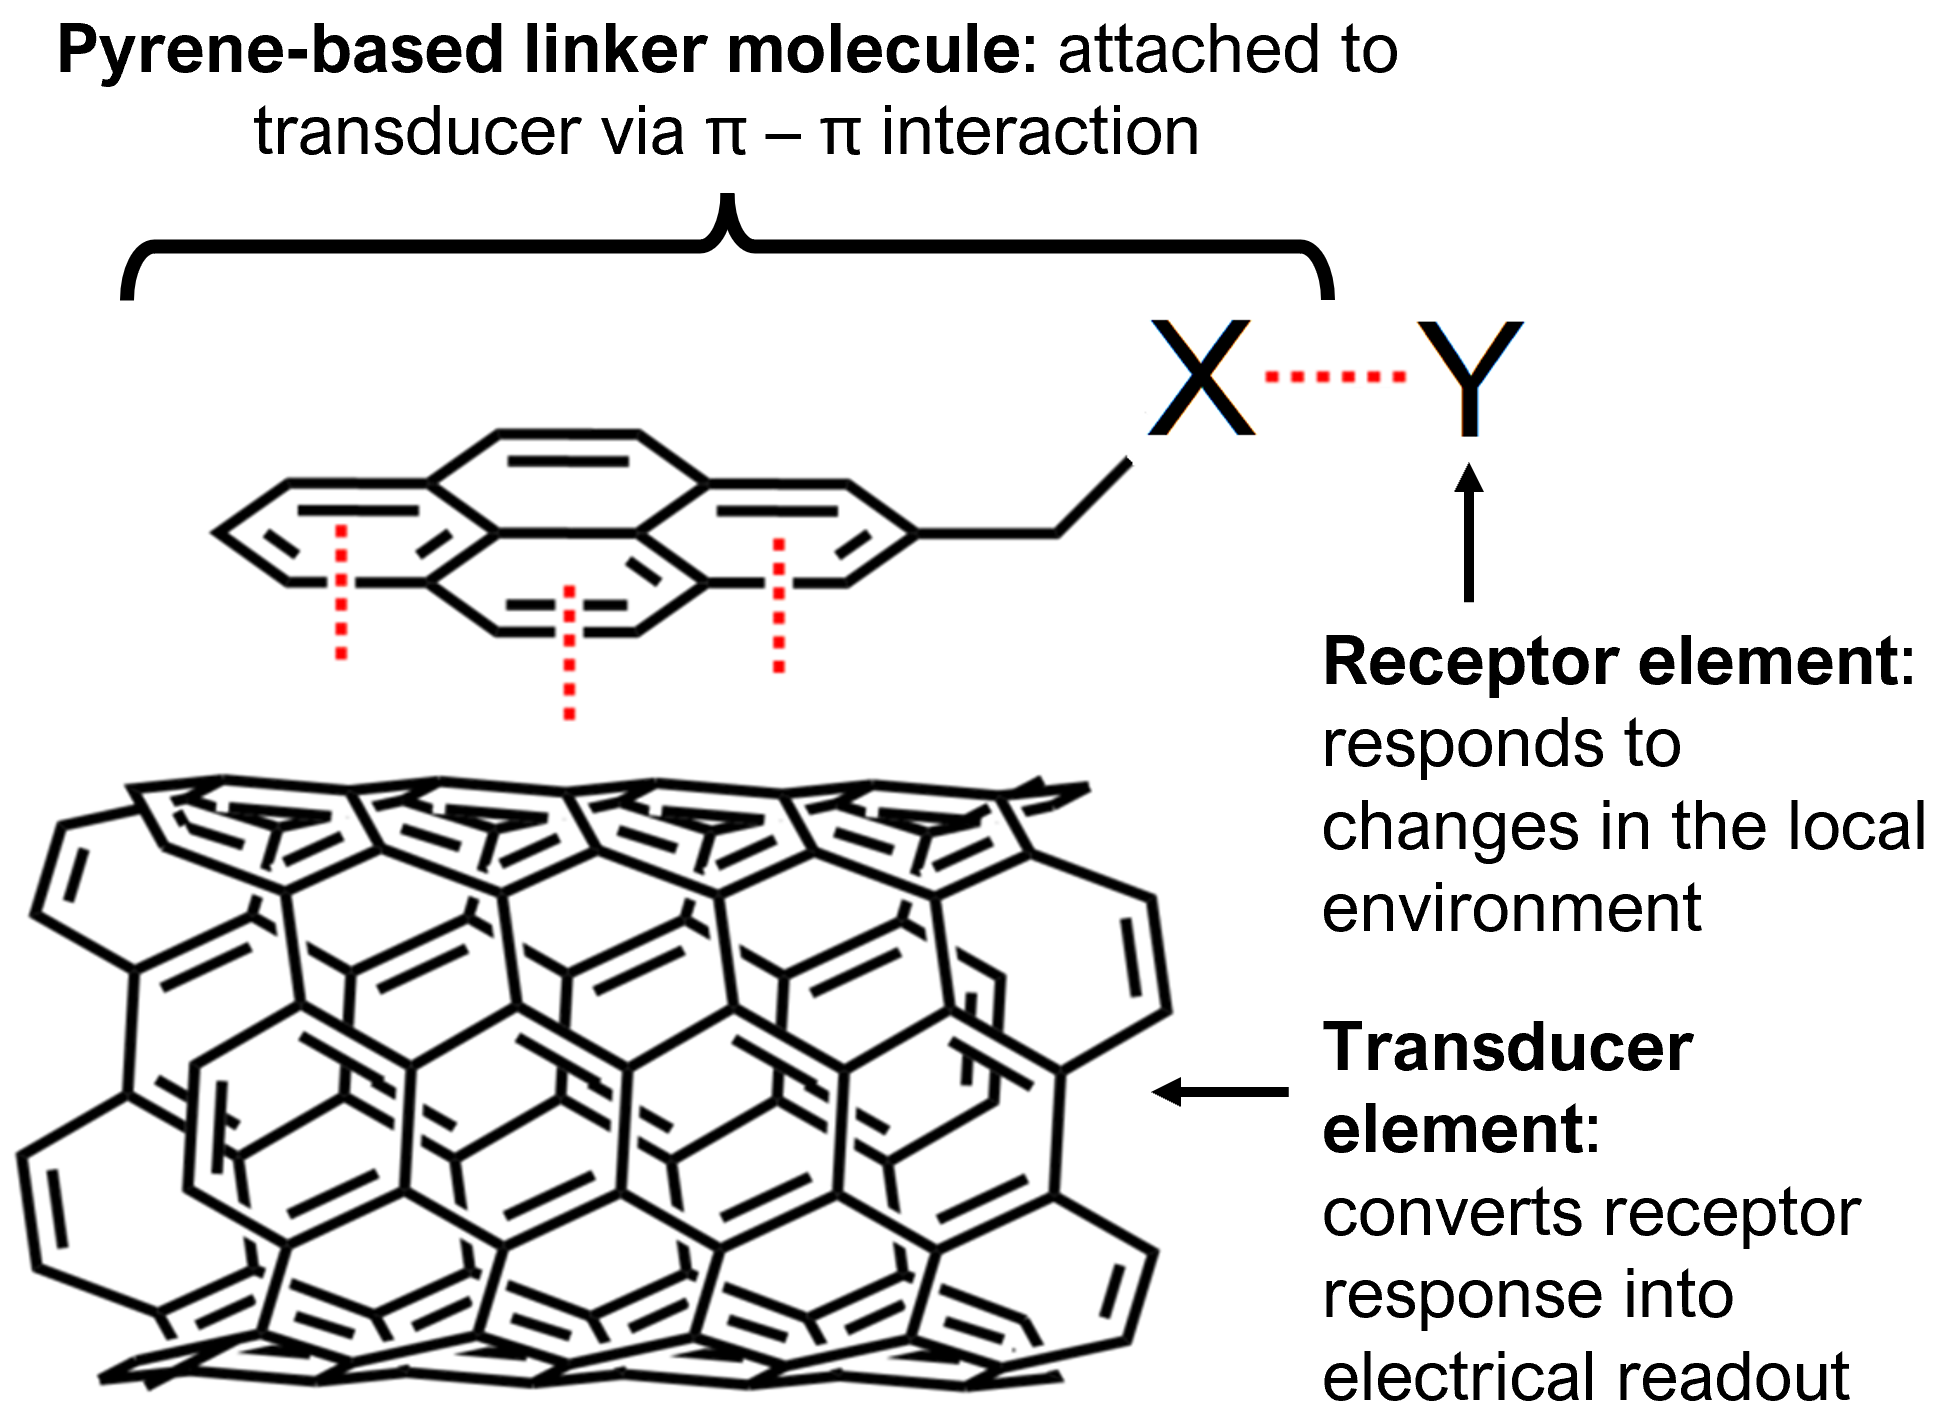
\includegraphics[width=0.75\textwidth,height=\textheight]{figures/ch3/pyrene-cnt.png}

}

\caption{\label{fig-pi-interaction-cnt}Attachment of pyrene-based linker
molecule pyrene-X and receptor Y to a carbon nanotube, representing the
transducer element of a field-effect transistor. Source: Adapted from
\autocite{Carbonnanotube}.}

\end{figure}

\(\pi\)-stacking or \(\pi-\pi\) interaction\footnote{It has been argued
  that this label is unhelpfully specific and a misrepresentation of
  what can be simply classed as a type of Van Der Waals bonding
  \autocite{Martinez2012,Perez2015}. However, as the use of the term is
  widespread in the literature, it is also used here for the sake of
  clarity.} is a specific type of non-covalent bonding which occurs due
to dispersion forces between unsaturated polycyclic molecules
\autocite{Perez2015}. A wide range of linker molecules with aromatic
moieties, such as pyrene, have been used for modification of polycyclic
carbon nanotubes and graphene via \(\pi\)-stacking
\autocite{Hermanson2013-16,Perez2015,Zhou2019,Mishyn2022}. Pyrene-based
\(\pi\)-stacking underlies all the functionalisation processes used in
this thesis.@fig-pi-interaction-cnt demonstrates how a pyrene-based
linker molecule can be used to attach a receptor element to a thin-film
transducer. The linker element attaches to the biomolecule via covalent
bonding with a nucleophilic functional group; linker attachment can
occur via biomolecule aminos, carboxyls, hydroxyls, thiols/sulfhydryls,
phenols, imidazoles and so on \autocite{Fruh2011,Dung2018}.

\hypertarget{sec-PBASE-attachment}{%
\subsection{Comparing Attachment Methods}\label{sec-PBASE-attachment}}

\begin{figure}

\begin{minipage}[t]{0.03\linewidth}

{\centering 

\raisebox{-\height}{


\includegraphics{figures/(a).png}

}

}

\end{minipage}%
%
\begin{minipage}[t]{0.01\linewidth}

{\centering 

~

}

\end{minipage}%
%
\begin{minipage}[t]{0.45\linewidth}

{\centering 

\raisebox{-\height}{

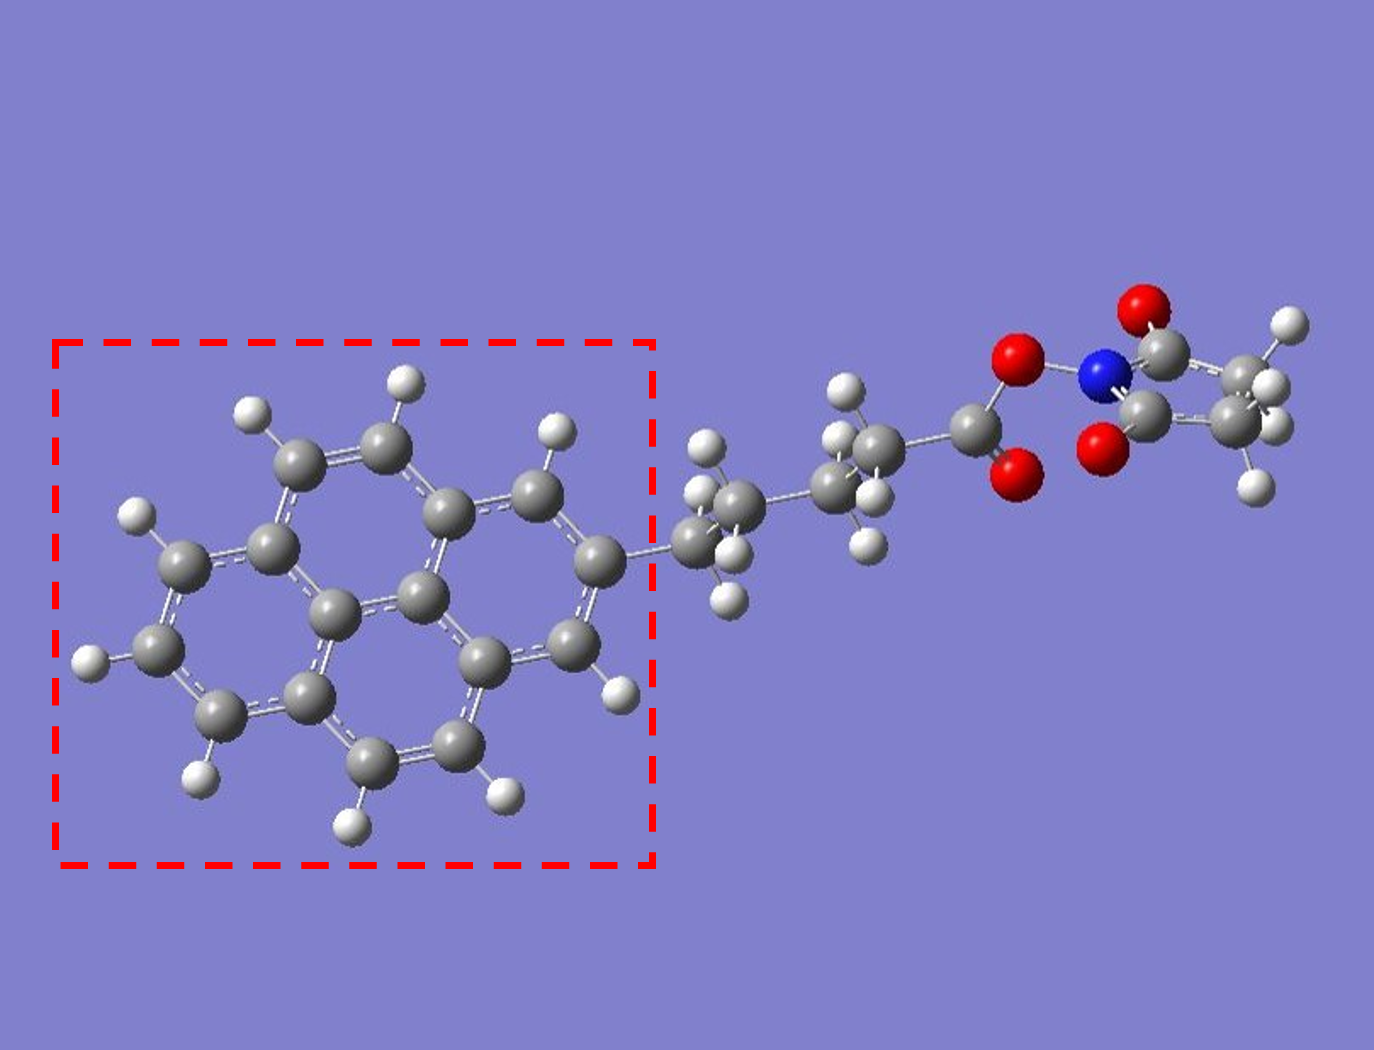
\includegraphics{figures/ch6/pbase_stable_1_pyrene.png}

}

}

\end{minipage}%
%
\begin{minipage}[t]{0.01\linewidth}

{\centering 

~

}

\end{minipage}%
%
\begin{minipage}[t]{0.03\linewidth}

{\centering 

\raisebox{-\height}{


\includegraphics{figures/(b).png}

}

}

\end{minipage}%
%
\begin{minipage}[t]{0.01\linewidth}

{\centering 

~

}

\end{minipage}%
%
\begin{minipage}[t]{0.45\linewidth}

{\centering 

\raisebox{-\height}{

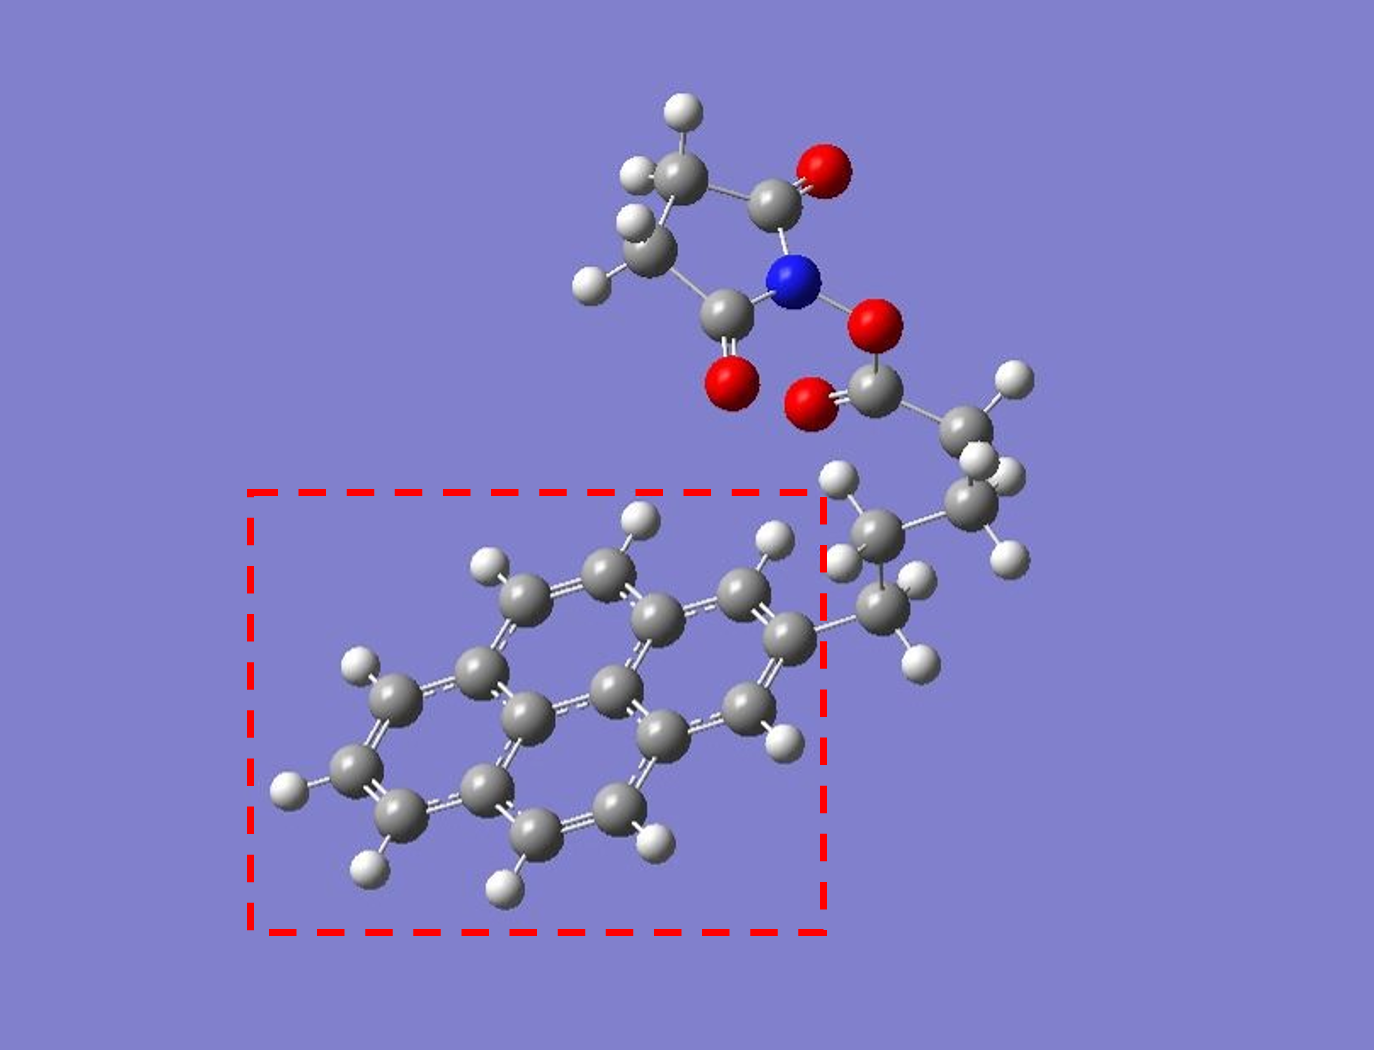
\includegraphics{figures/ch6/pbase_stable_2_pyrene.png}

}

}

\end{minipage}%
%
\begin{minipage}[t]{0.01\linewidth}

{\centering 

~

}

\end{minipage}%

\caption{\label{fig-pbase-structure}Two conformations of PBASE molecule
with geometry optimised via \emph{ab initio} calculations performed with
Gaussian 16 software \autocite{g16}. White balls correspond to hydrogen,
grey to carbon, red to oxygen and blue to nitrogen. The pyrene moiety is
highlighted in the image with a red dashed outline.}

\end{figure}

1-pyrenebutanoic acid N-hydroxysuccinimide ester (also known as
1-pyrenebutyric acid N-hydroxysuccinimide ester and 1-pyrenebutanoic
acid succinimidyl ester, and by the acronyms PBASE, PBSE, PyBASE, PASE,
PYSE, PSE, Pyr-NHS and PANHS) is a pyrene-based linker molecule commonly
used for tethering biomolecules to the carbon rings of graphene and
carbon nanotubes. Two locally stable molecular conformations were found
to exist using computational modelling, shown in
Figure~\ref{fig-pbase-structure} (a) and
Figure~\ref{fig-pbase-structure} (b) respectively. The Hartree-Fock
energy of the straight conformation in Figure~\ref{fig-pbase-structure}
(a) is -3427728.67 kJ/mol, while the Hartree-Fock energy of the bent
conformation in Figure~\ref{fig-pbase-structure} (b) is -3427729.66
kJ/mol. The difference between energies is small enough that the
existence of both molecular conformations is feasible. Similar straight
and bent structures have previously been modelled for PBASE attached to
graphene \autocite{Oishi2022}. The pyrene moiety, highlighted with a red
dashed outline in Figure~\ref{fig-pbase-structure}, non-covalently bonds
to the carbon rings of the transducer. The N-hydroxysuccinimide (NHS)
ester group, seen on the right-hand side of
Figure~\ref{fig-pbase-structure}, can undergo a nucleophilic
substitution reaction with primary amines attached to biomolecules,
tethering them with an amide or imide bond
\autocite{Chen2001,Hermanson2013-16,Hermanson2013-3,Shkodra2021,Mishyn2022}.

The non-covalent functionalisation of proteins onto a single-walled
carbon nanotube using PBASE was first reported by Chen \emph{et al.} in
2001 \autocite{Chen2001}. Two successful methods for protein
functionalisation and immobilisation were reported, with the only
differences being the solvent used to dissolve the PBASE powder
(dimethylformamide, methanol) and the final concentration of the
resulting solutions (6 mM, 1 mM respectively). PBASE powder appears to
dissolve poorly in methanol at higher concentrations, which might
explain the use of different concentrations of PBASE with each solvent.
An extensive comparison of methods used in the literature for PBASE
functionalisation of carbon nanotube and graphene devices with aptamers
and proteins is given in Table~\ref{tbl-pbase-functionalisation}.
Several listed works directly cite Chen \emph{et al.} when discussing
functionalisation with PBASE
\autocite{Besteman2003,Cella2010,Campos2019,Zheng2016,Ohno2010}. The
other works listed do not explicitly reference Chen \emph{et al.} in
their methodology; however, the frequency of methods describing the use
of 6 mM PBASE in dimethylformamide (DMF) and 1 mM PBASE in methanol
indicate that other groups often emulate the original process from Chen
\emph{et al.}.

However, it is also apparent from
Table~\ref{tbl-pbase-functionalisation} that there is a large degree of
variation in the methods used for PBASE functionalisation. Various
electrical characterisation, microscopy and spectroscopy techniques have
been used to demonstrate successful functionalisation. Until recently,
there has been little justification provided for the selection of
variables used in the functionalisation procedure (\emph{e.g.} length of
time submerged in solvent containing PBASE), despite the wide-ranging
use of this process in the literature
\autocite{Hinnemo2017,Zhen2018,Wang2020}. Furthermore, a detailed
investigation of PBASE functionalisation process variables has only been
undertaken for graphene-based devices
\autocite{Zhen2018,Hao2020,Wang2020,Mishyn2022}. This is surprising,
given that multiple sources make an explicit link between sensitivity of
functionalised devices and the density of surface functionalisation with
PBASE \autocite{White2008,Hermanson2013-3,Chen2014}.

Zhen \emph{et al.} \autocite{Zhen2018}, Wang \emph{et al.}
\autocite{Wang2020} and Mishyn \emph{et al.} \autocite{Mishyn2022} have
all claimed that carefully tuning the surface concentration of PBASE is
required to avoid multilayer coverage of the graphene surface, as this
negatively impacts sensing. Mishyn \emph{et al.} \autocite{Mishyn2022}
used cyclic voltammetry to demonstrate that less receptor attachment to
the graphene surface occurs when multiple layers of PBASE are present.
However, none of these groups have presented analyte sensing results
from their functionalised graphene devices. In contrast, Hao \emph{et
al.} \autocite{Hao2020} found that maximising the PBASE surface coverage
of a channel resulted in more sensitive aptameric sensing, thereby
reaching the opposite conclusion. The inconsistency in these recent
findings mean more work is needed to understand the PBASE
functionalisation process to achieve optimal biosensor sensitivity. It
may also be the case that a specific functionalisation process is
required for optimal sensitivity with the use of a specific type of
receptor.

Once fastened to a bioreceptor via an amide or imide bond, the
attachment to the linker molecule is not easily broken. However, prior
to use in functionalisation processes, the NHS ester may react with any
water present. This ester hydrolysis converts PBASE to its corresponding
carboxylic acid, 1-pyrenebutyric acid (PBA), leaving it unavailable to
react further with amine groups
\autocite{Hermanson2013-3,Hermanson2013-5,Mishyn2022}. If the amine
group functionalisation is performed at close to neutral pH, within a
\(\sim\) 1 hour period, and with a high concentration of bioreceptor
present, competing hydrolysis should not have a significantly adverse
impact on the functionalisation process \autocite{Hermanson2013-3}. If
PBASE is exposed to water during storage,
1-Ethyl-3-(3-dimethylaminopropyl)carbodiimide (EDC) can be used to
restore the NHS ester and enable the substitution reaction to take place
(see Section~\ref{sec-PBA}).

\newpage
\thispagestyle{empty}
\KOMAoptions{paper=landscape,pagesize}

\hypertarget{tbl-pbase-functionalisation}{}
\begin{longtable}[]{@{}lllllll@{}}
\caption{\label{tbl-pbase-functionalisation}Comparison of PBASE
functionalisation processes used for immobilisation of proteins and
aptamers onto carbon nanotubes and graphene. Experimentally optimised
variables are marked with a star (*). Blank entries indicate there was
no mention of the parameter in a particular paper.}\tabularnewline
\toprule\noalign{}
Solvent & Channel & Conc. (mM) & Incubation type & Time (hr) & Rinse
steps & References \\
\midrule\noalign{}
\endfirsthead
\toprule\noalign{}
Solvent & Channel & Conc. (mM) & Incubation type & Time (hr) & Rinse
steps & References \\
\midrule\noalign{}
\endhead
\bottomrule\noalign{}
\endlastfoot
DMF & CNT & 5 & Immersed & 1 & PBS & Maehashi, 2007.
\cite{Maehashi2007} \\
& & 6 & Immersed & 1 & DMF, PBS & García-Aljaro, 2010.
\cite{Garcia-Aljaro2010} \\
& & 6 & Immersed & 1 & DMF & Chen, 2001. \cite{Chen2001} \\
& & 6 & Immersed & 1 & DMF & Cella, 2010. \cite{Cella2010} \\
& & 6 & Immersed & 1 & DMF & Das, 2011. \cite{Das2011} \\
& & 6 & - & 2 & DMF & Besteman, 2003. \cite{Besteman2003} \\
& Graphene & - & - & 2 & DMF & Tsang, 2019. \cite{Tsang2019} \\
& & - & - & 20 & - & Wiedman, 2017. \cite{Wiedman2017} \\
& & 0.2 & Immersed & 20 & DMF, IPA, DI water & Gao, 2018.
\cite{Gao2018} \\
& & 1 & Dropcast & 6 & DMF, IPA, DI water & Nekrasov, 2021.
\cite{Nekrasov2021} \\
& & 5 & Immersed & 1 & DMF, DI water & Hwang, 2016. \cite{Hwang2016} \\
& & 5* & Immersed & 3* & DMF & Hao, 2020. \cite{Hao2020} \\
& & 5 & Immersed & 4* & DMF, DI water & Mishyn, 2022.
\cite{Mishyn2022} \\
& & 6 & Dropcast & 2 & DMF, DI water & Nur Nasufiya, 2020.
\cite{NurNasyifa2020} \\
& & 10 & Dropcast & 2 & DMF, DI water & Campos, 2019.
\cite{Campos2019} \\
& & 10 & Immersed & 2 & DMF, PBS & Kuscu, 2020. \cite{Kuscu2020} \\
& & 10 & Immersed & 1 & DMF & Xu, 2017. \cite{Xu2017} \\
& & 10 & Immersed & 12 & DMF, EtOH, DI water & Khan, 2020.
\cite{Khan2020} \\
& & 50 & Immersed & 4* & MeOH & Wang, 2020. \cite{Wang2020} \\
2-Methoxyethanol & Graphene & 1 & Immersed & 1 & DI water & Ono, 2020.
\cite{Ono2020} \\
Methanol & CNT & 1 & Immersed & 1 & MeOH, DI water & Zheng, 2016.
\cite{Zheng2016} \\
& & 1 & Immersed & 2 & MeOH & Kim, 2009. \cite{Kim2009} \\
& & 100 & Dropcast & 1 & DI water & Yoo, 2022. \cite{Yoo2022} \\
& Graphene & 5 & Immersed & 2 & - & Sethi, 2020. \cite{Sethi2020} \\
& & 5 & Immersed & 1 & MeOH, PBS & Ohno, 2010. \cite{Ohno2010} \\
DMSO & CNT & 10 & - & 1 & DI water & Lopez, 2015. \cite{Lopez2015} \\
& & 10 & Immersed & 1 & PBS & Strack, 2013. \cite{Strack2013} \\
\end{longtable}

\newpage
\KOMAoptions{paper=portrait,pagesize}

\begin{figure}[H]

\begin{minipage}[t]{0.03\linewidth}

{\centering 

\raisebox{-\height}{


\includegraphics{figures/(a).png}

}

}

\end{minipage}%
%
\begin{minipage}[t]{0.01\linewidth}

{\centering 

~

}

\end{minipage}%
%
\begin{minipage}[t]{0.92\linewidth}

{\centering 

\raisebox{-\height}{

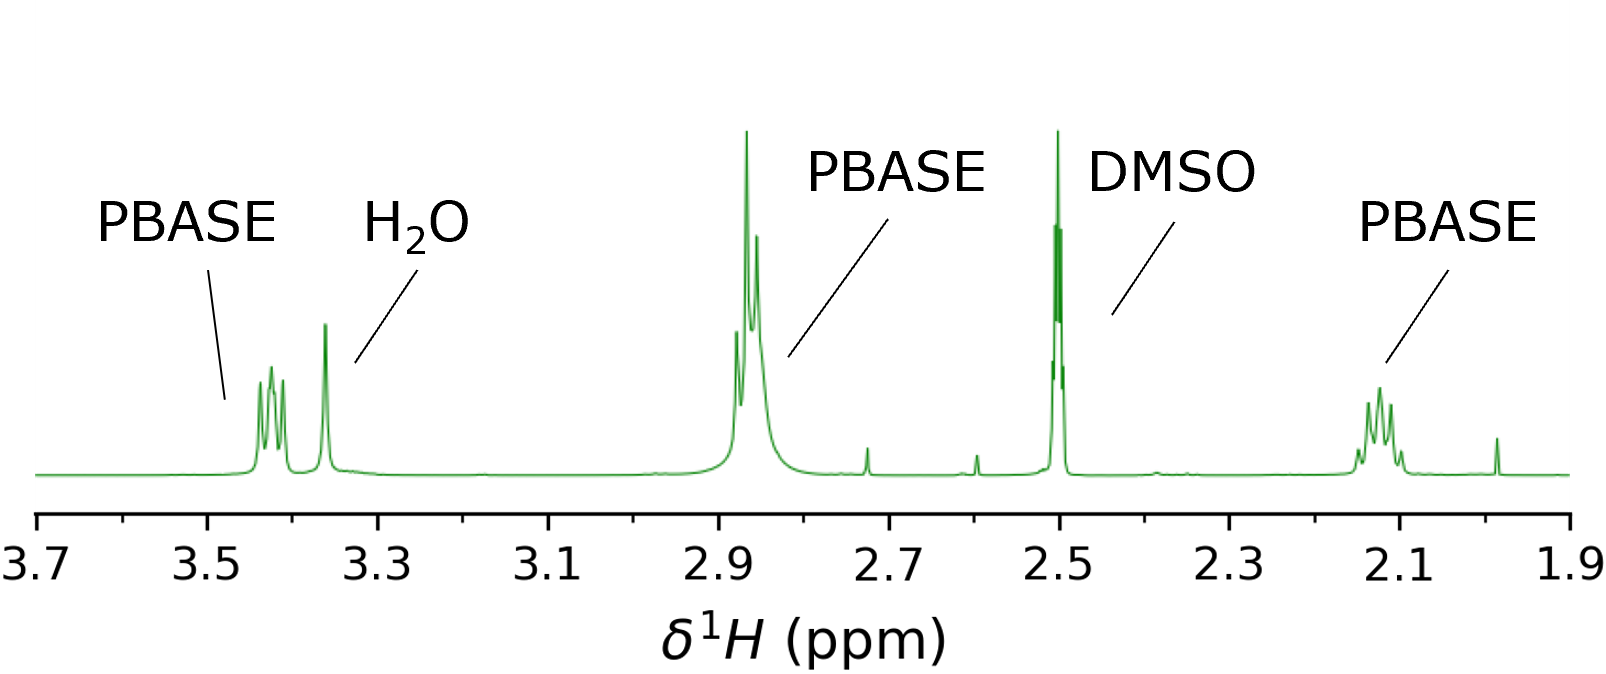
\includegraphics{figures/ch6/labelled_modified_sigma_pbase_nmr.png}

}

}

\end{minipage}%
%
\begin{minipage}[t]{0.04\linewidth}

{\centering 

~

}

\end{minipage}%
\newline
\begin{minipage}[t]{0.03\linewidth}

{\centering 

\raisebox{-\height}{


\includegraphics{figures/(b).png}

}

}

\end{minipage}%
%
\begin{minipage}[t]{0.01\linewidth}

{\centering 

~

}

\end{minipage}%
%
\begin{minipage}[t]{0.92\linewidth}

{\centering 

\raisebox{-\height}{

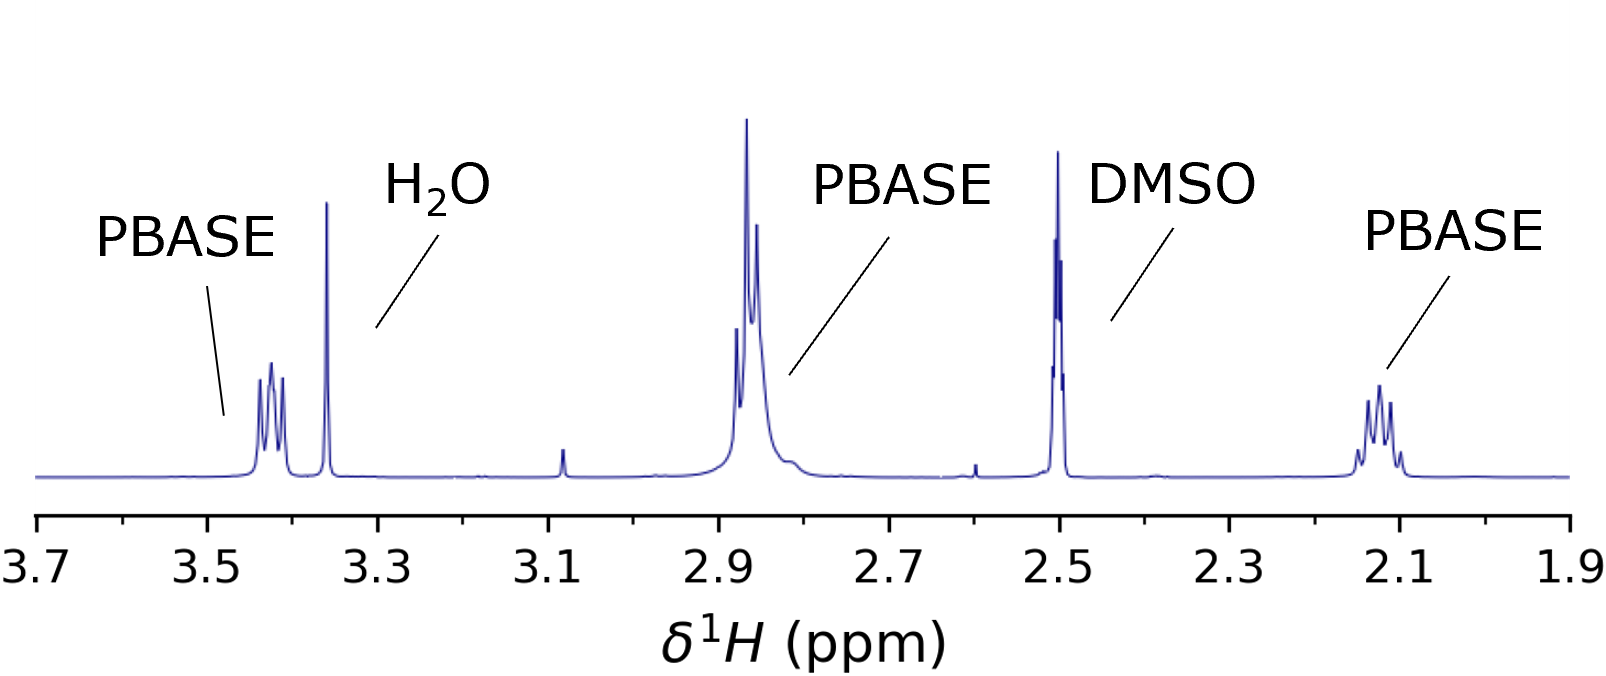
\includegraphics{figures/ch6/labelled_modified_setareh_pbase_nmr.png}

}

}

\end{minipage}%
%
\begin{minipage}[t]{0.04\linewidth}

{\centering 

~

}

\end{minipage}%
\newline
\begin{minipage}[t]{0.03\linewidth}

{\centering 

\raisebox{-\height}{


\includegraphics{figures/(c).png}

}

}

\end{minipage}%
%
\begin{minipage}[t]{0.01\linewidth}

{\centering 

~

}

\end{minipage}%
%
\begin{minipage}[t]{0.92\linewidth}

{\centering 

\raisebox{-\height}{

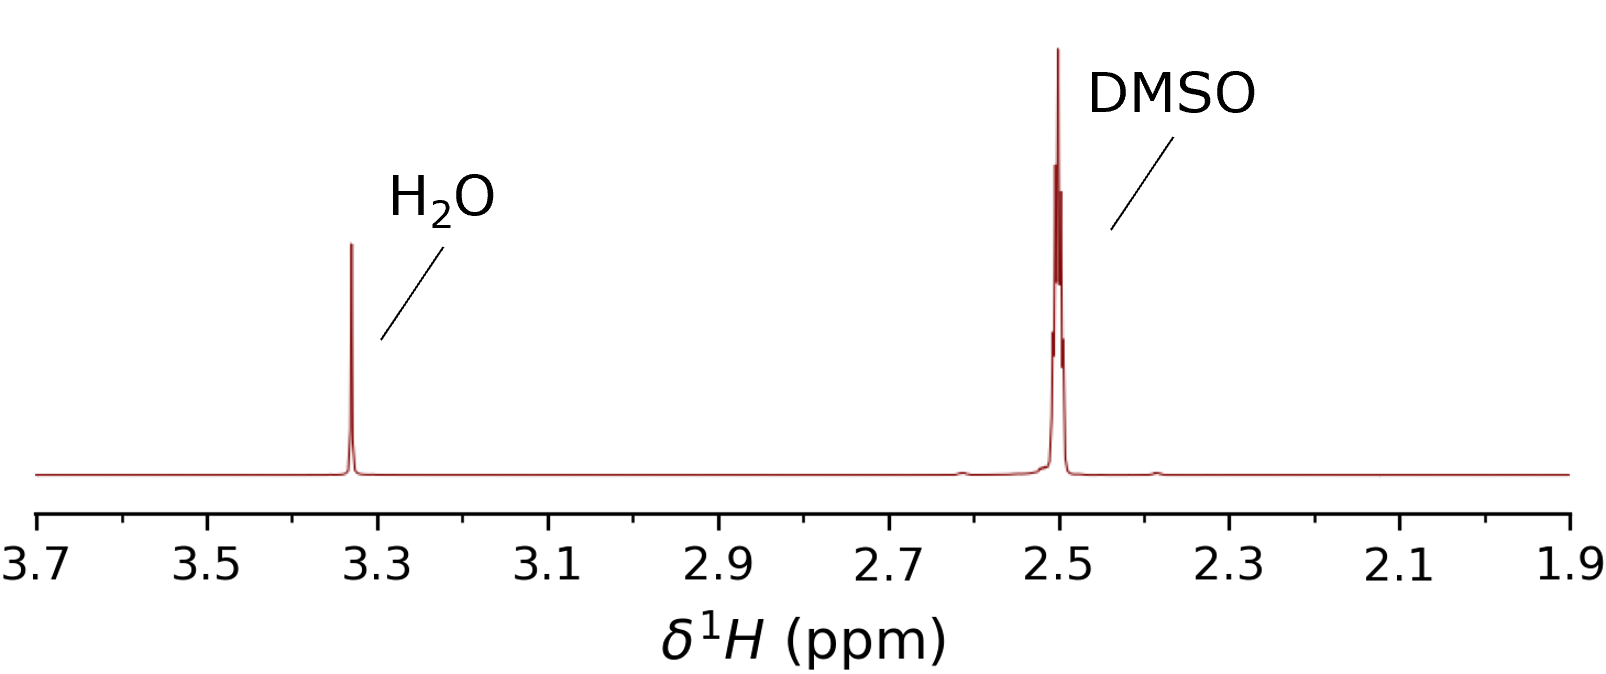
\includegraphics{figures/ch6/labelled_modified_dmso_nmr.png}

}

}

\end{minipage}%
%
\begin{minipage}[t]{0.04\linewidth}

{\centering 

~

}

\end{minipage}%

\caption{\label{fig-pbase-nmr}\(^{1}\)H Nuclear Magnetic Resonance (NMR)
spectra, performed with DMSO-d\(_6\) used as the NMR solvent. (a) and
(b) show NMR spectrum for commercially purchased PBASE, from
Sigma-Aldrich and Setareh Biotech respectively, while (c) shows the
blank spectrum taken with only DMSO-d\(_6\) present. Spectra were taken
by Jennie Ramirez-Garcia, School of Chemical and Physical Sciences, Te
Herenga Waka - Victoria University of Wellington. Unlabelled peaks
correspond to sample impurities.}

\end{figure}

\hypertarget{sec-PBASE-purity}{%
\subsection{Examining 1-Pyrenebutanoic Acid N-Hydroxysuccinimide Ester
Purity}\label{sec-PBASE-purity}}

I purchased PBASE from two suppliers, Sigma-Aldrich and Setareh Biotech.
Sigma listed DMF and methanol as suitable solvents for dissolving PBASE,
alongside chloroform and dimethyl sulfoxide (DMSO). Setareh Biotech
indicated methanol can be used for dissolving PBASE. The two suppliers
had conflicting information for suitable storage of PBASE, where Sigma
recommended room temperature storage, while Setareh Biotech recommended
storage of -5 to -30°C alongside protection from light and moisture. I
used nuclear magnetic resonance (NMR) spectroscopy to verify the purity
of PBASE from various suppliers. As water can react with PBASE to form
unwanted byproducts, it appears that protection from moisture is
particularly important. A particular emphasis was placed on detecting
water presence in the received samples, considering the long travel time
of the PBASE with uncertain storage conditions.

Figure~\ref{fig-pbase-nmr} compares the shapes of hydrogen NMR spectra
of PBASE from each supplier when dissolved in deuterated DMSO, alongside
a blank deuterated DMSO spectrum. Both PBASE samples possessed
characteristic chemical shift features between \(2.1-2.2\) ppm,
\(2.8-2.9\) ppm, and \(3.4-3.5\) ppm. These chemical shifts roughly
correspond to those seen in previous NMR spectra for PBASE
\autocite{NMR2}. The feature at 2.50 ppm represents the deuterated DMSO
solvent, while the single peak between \(3.3-3.4\) ppm represents the
water present in the sample. By comparing the area of these peaks, a
rough estimate of the amount of water originally present in the PBASE
sample can be obtained. The H\(_{2}\)O:DMSO ratio is 1:7 in the blank
spectrum, but \(\sim\) 1:3 in the provided samples, possibly indicating
the introduction of water to the PBASE during production or storage.
However, DMSO is strongly hygroscopic and slight differences in DMSO
storage time, as well as differences in humidity during sample
preparation, may have had a significant impact on this result
\autocite{Lebel1962}. Other impurities are also seen on both PBASE
spectra, though their small size indicates they make up only a small
percentage of each sample. Strack \emph{et al.} \autocite{Strack2013}
recommend leaving frozen PBASE at room temperature for 15 minutes before
exposing it to air to prevent condensation near the PBASE, as this can
cause unnecessary H\(_2\)O contamination.

\hypertarget{sec-PBASE-electrical-characterisation}{%
\subsection{Electrical
Characterisation}\label{sec-PBASE-electrical-characterisation}}

The electrical characteristics of the carbon nanotube or graphene
transistor are often used to verify successful functionalisation and
make a statement about the effect of chemical modification on the
channel. However, this verification usually does not account for the
effect of the solvent on the transistor channel.
Figure~\ref{fig-PBASE-vs-solvent-only} (a) and
Figure~\ref{fig-PBASE-vs-solvent-only} (b) show that by exposing a
steam-deposited carbon nanotube network channel to solvents commonly
used in PBASE functionalisation processes
(Table~\ref{tbl-pbase-functionalisation}), such as methanol (MeOH) or
dimethyl sulfoxide (DMSO), a significant negative shift in channel
threshold voltage occurs even after thorough rinsing with deionised
water. It appears that the carbon nanotubes have adsorped solvent which
persists even after thoroughly rinsing the device. From the shape of the
change in the transfer curve, it seems the residual polar solvent
molecules capacitively gate the channel
\autocite{Artyukhin2006,Heller2008}. Besteman \emph{et al.} reported
observing a similar effect from prolonged exposure of a single carbon
nanotube to dimethylformamide (DMF) \autocite{Besteman2003}.

\begin{figure}

\begin{minipage}[t]{0.03\linewidth}

{\centering 

\raisebox{-\height}{


\includegraphics{figures/(a).png}

}

}

\end{minipage}%
%
\begin{minipage}[t]{0.01\linewidth}

{\centering 

~

}

\end{minipage}%
%
\begin{minipage}[t]{0.45\linewidth}

{\centering 

\raisebox{-\height}{

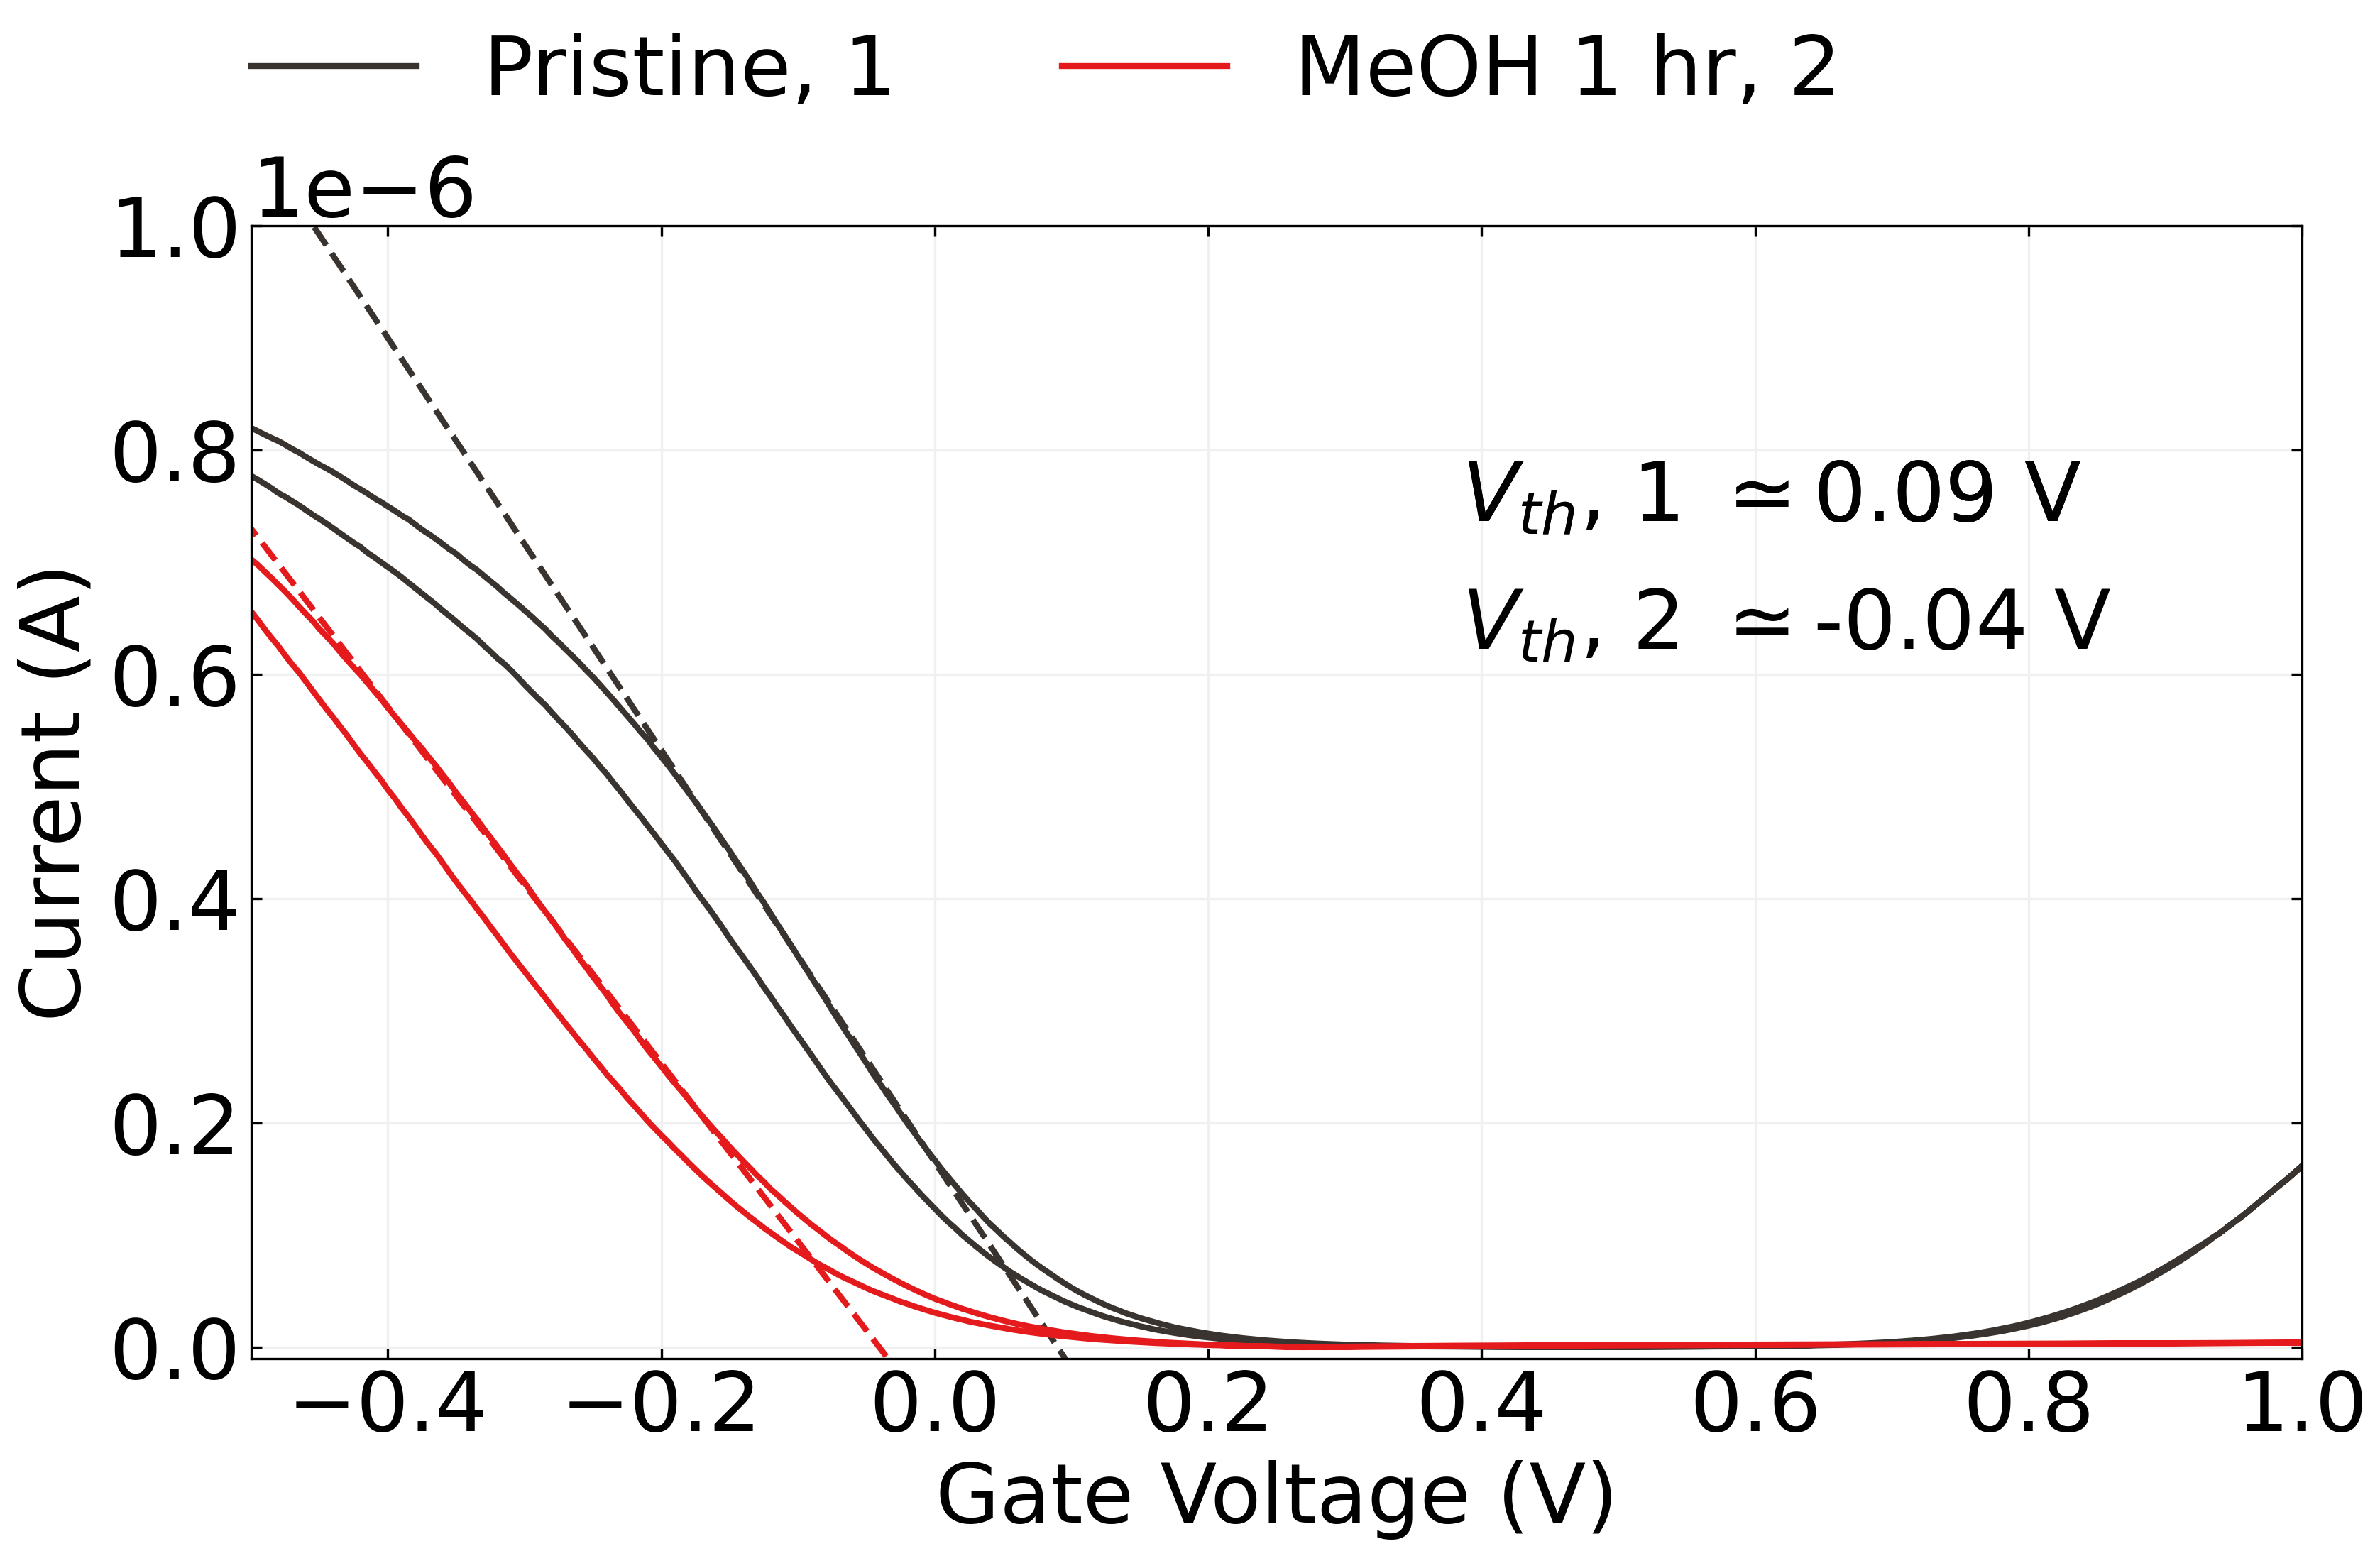
\includegraphics{figures/ch6/Q23D5_ch1_MeOHonly.png}

}

}

\end{minipage}%
%
\begin{minipage}[t]{0.01\linewidth}

{\centering 

~

}

\end{minipage}%
%
\begin{minipage}[t]{0.03\linewidth}

{\centering 

\raisebox{-\height}{


\includegraphics{figures/(b).png}

}

}

\end{minipage}%
%
\begin{minipage}[t]{0.01\linewidth}

{\centering 

~

}

\end{minipage}%
%
\begin{minipage}[t]{0.45\linewidth}

{\centering 

\raisebox{-\height}{

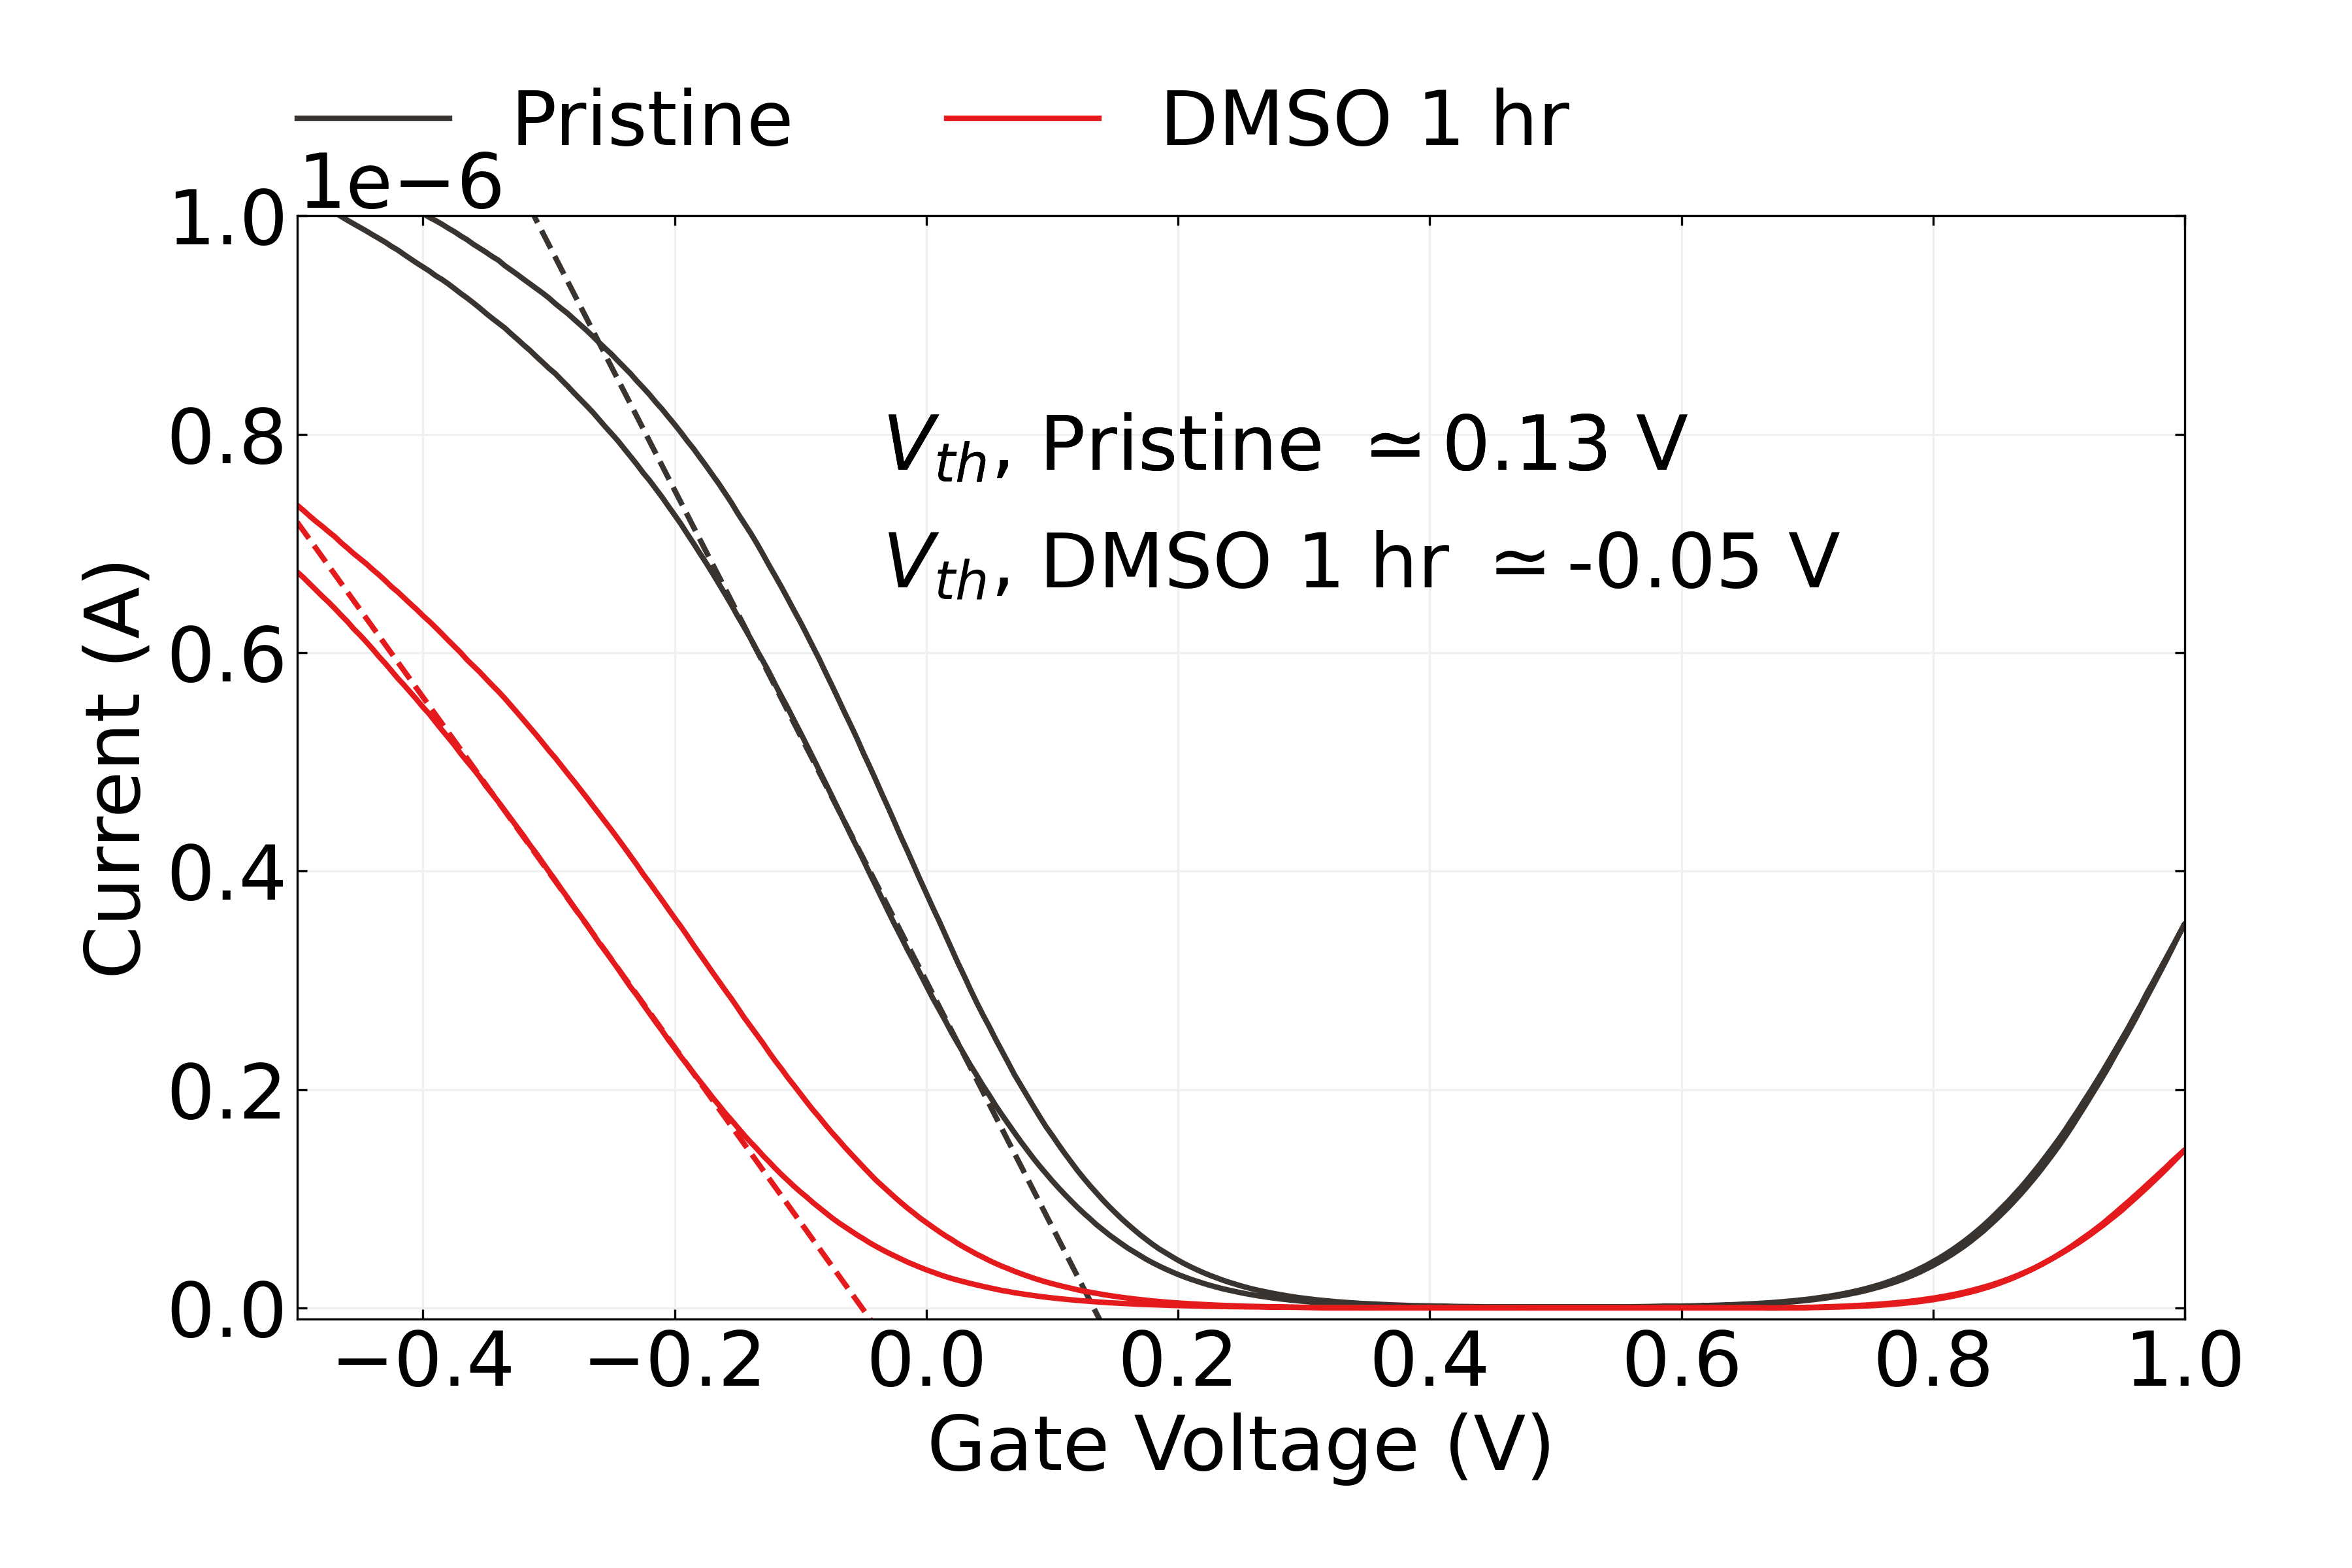
\includegraphics{figures/ch6/Q23D12_ch1_DMSOonly.png}

}

}

\end{minipage}%
%
\begin{minipage}[t]{0.01\linewidth}

{\centering 

~

}

\end{minipage}%
\newline
\begin{minipage}[t]{0.03\linewidth}

{\centering 

\raisebox{-\height}{


\includegraphics{figures/(c).png}

}

}

\end{minipage}%
%
\begin{minipage}[t]{0.01\linewidth}

{\centering 

~

}

\end{minipage}%
%
\begin{minipage}[t]{0.45\linewidth}

{\centering 

\raisebox{-\height}{

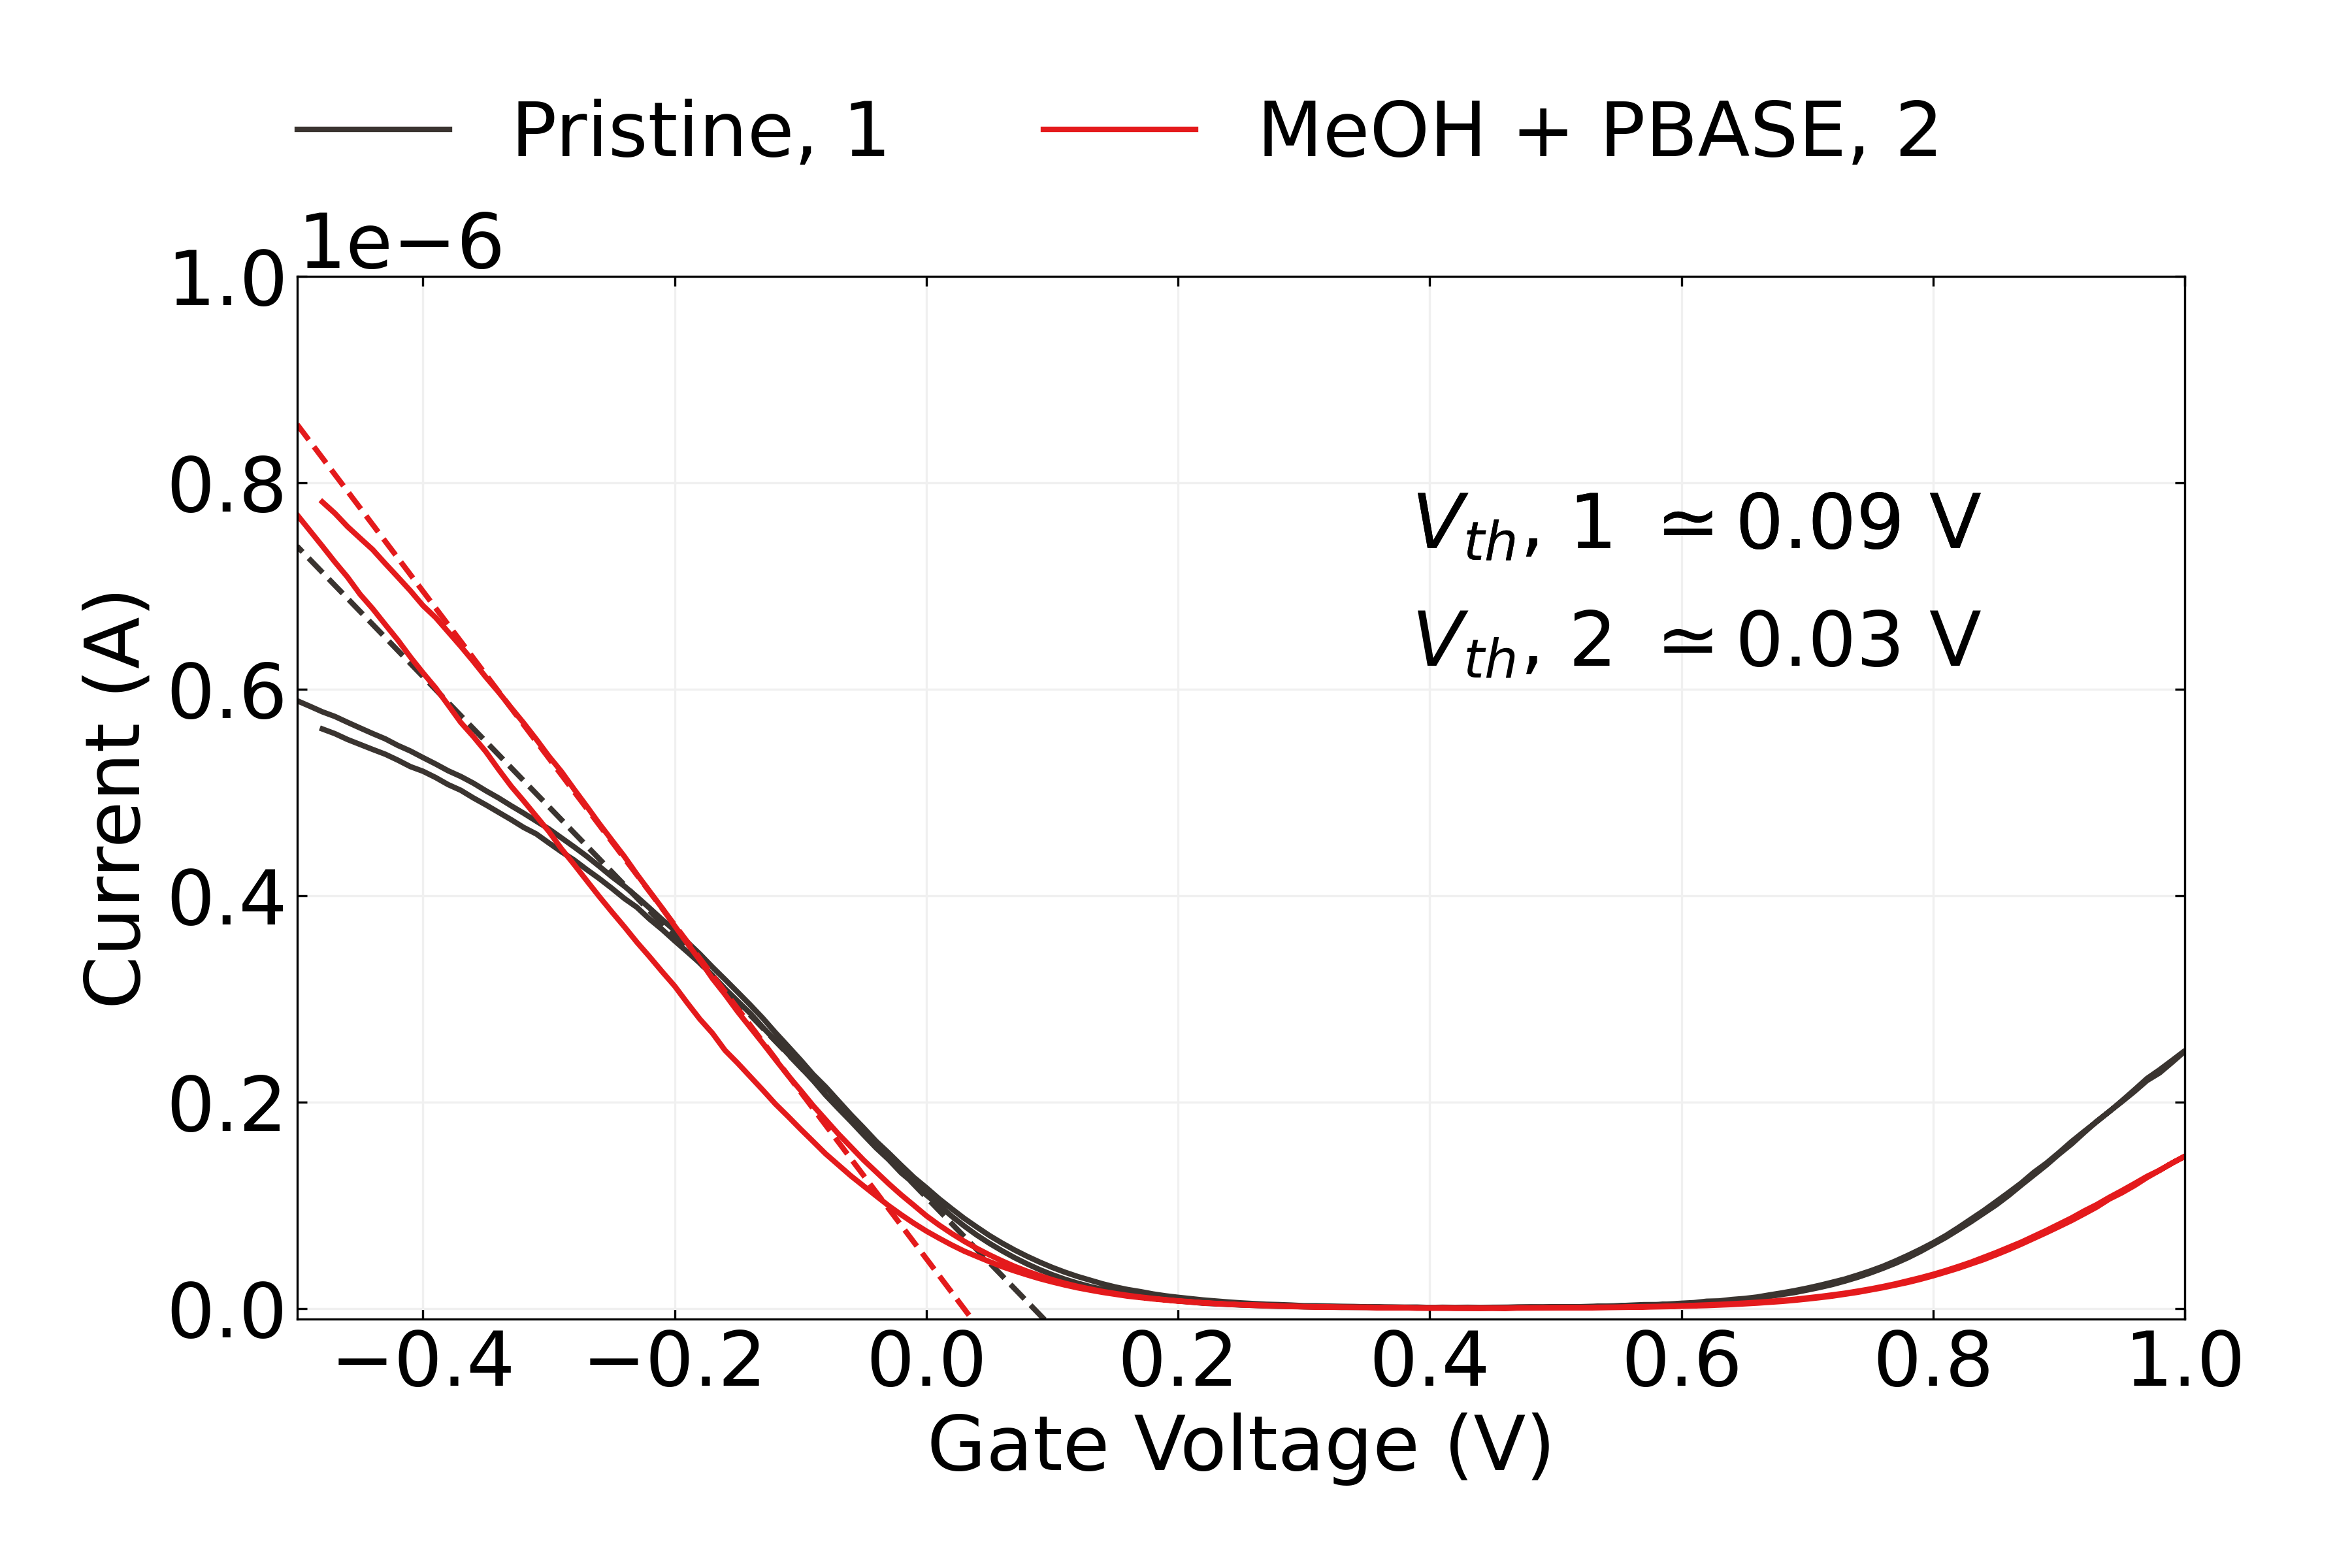
\includegraphics{figures/ch6/Q2C6_ch2_MeOHPBASE.png}

}

}

\end{minipage}%
%
\begin{minipage}[t]{0.01\linewidth}

{\centering 

~

}

\end{minipage}%
%
\begin{minipage}[t]{0.03\linewidth}

{\centering 

\raisebox{-\height}{


\includegraphics{figures/(d).png}

}

}

\end{minipage}%
%
\begin{minipage}[t]{0.01\linewidth}

{\centering 

~

}

\end{minipage}%
%
\begin{minipage}[t]{0.45\linewidth}

{\centering 

\raisebox{-\height}{

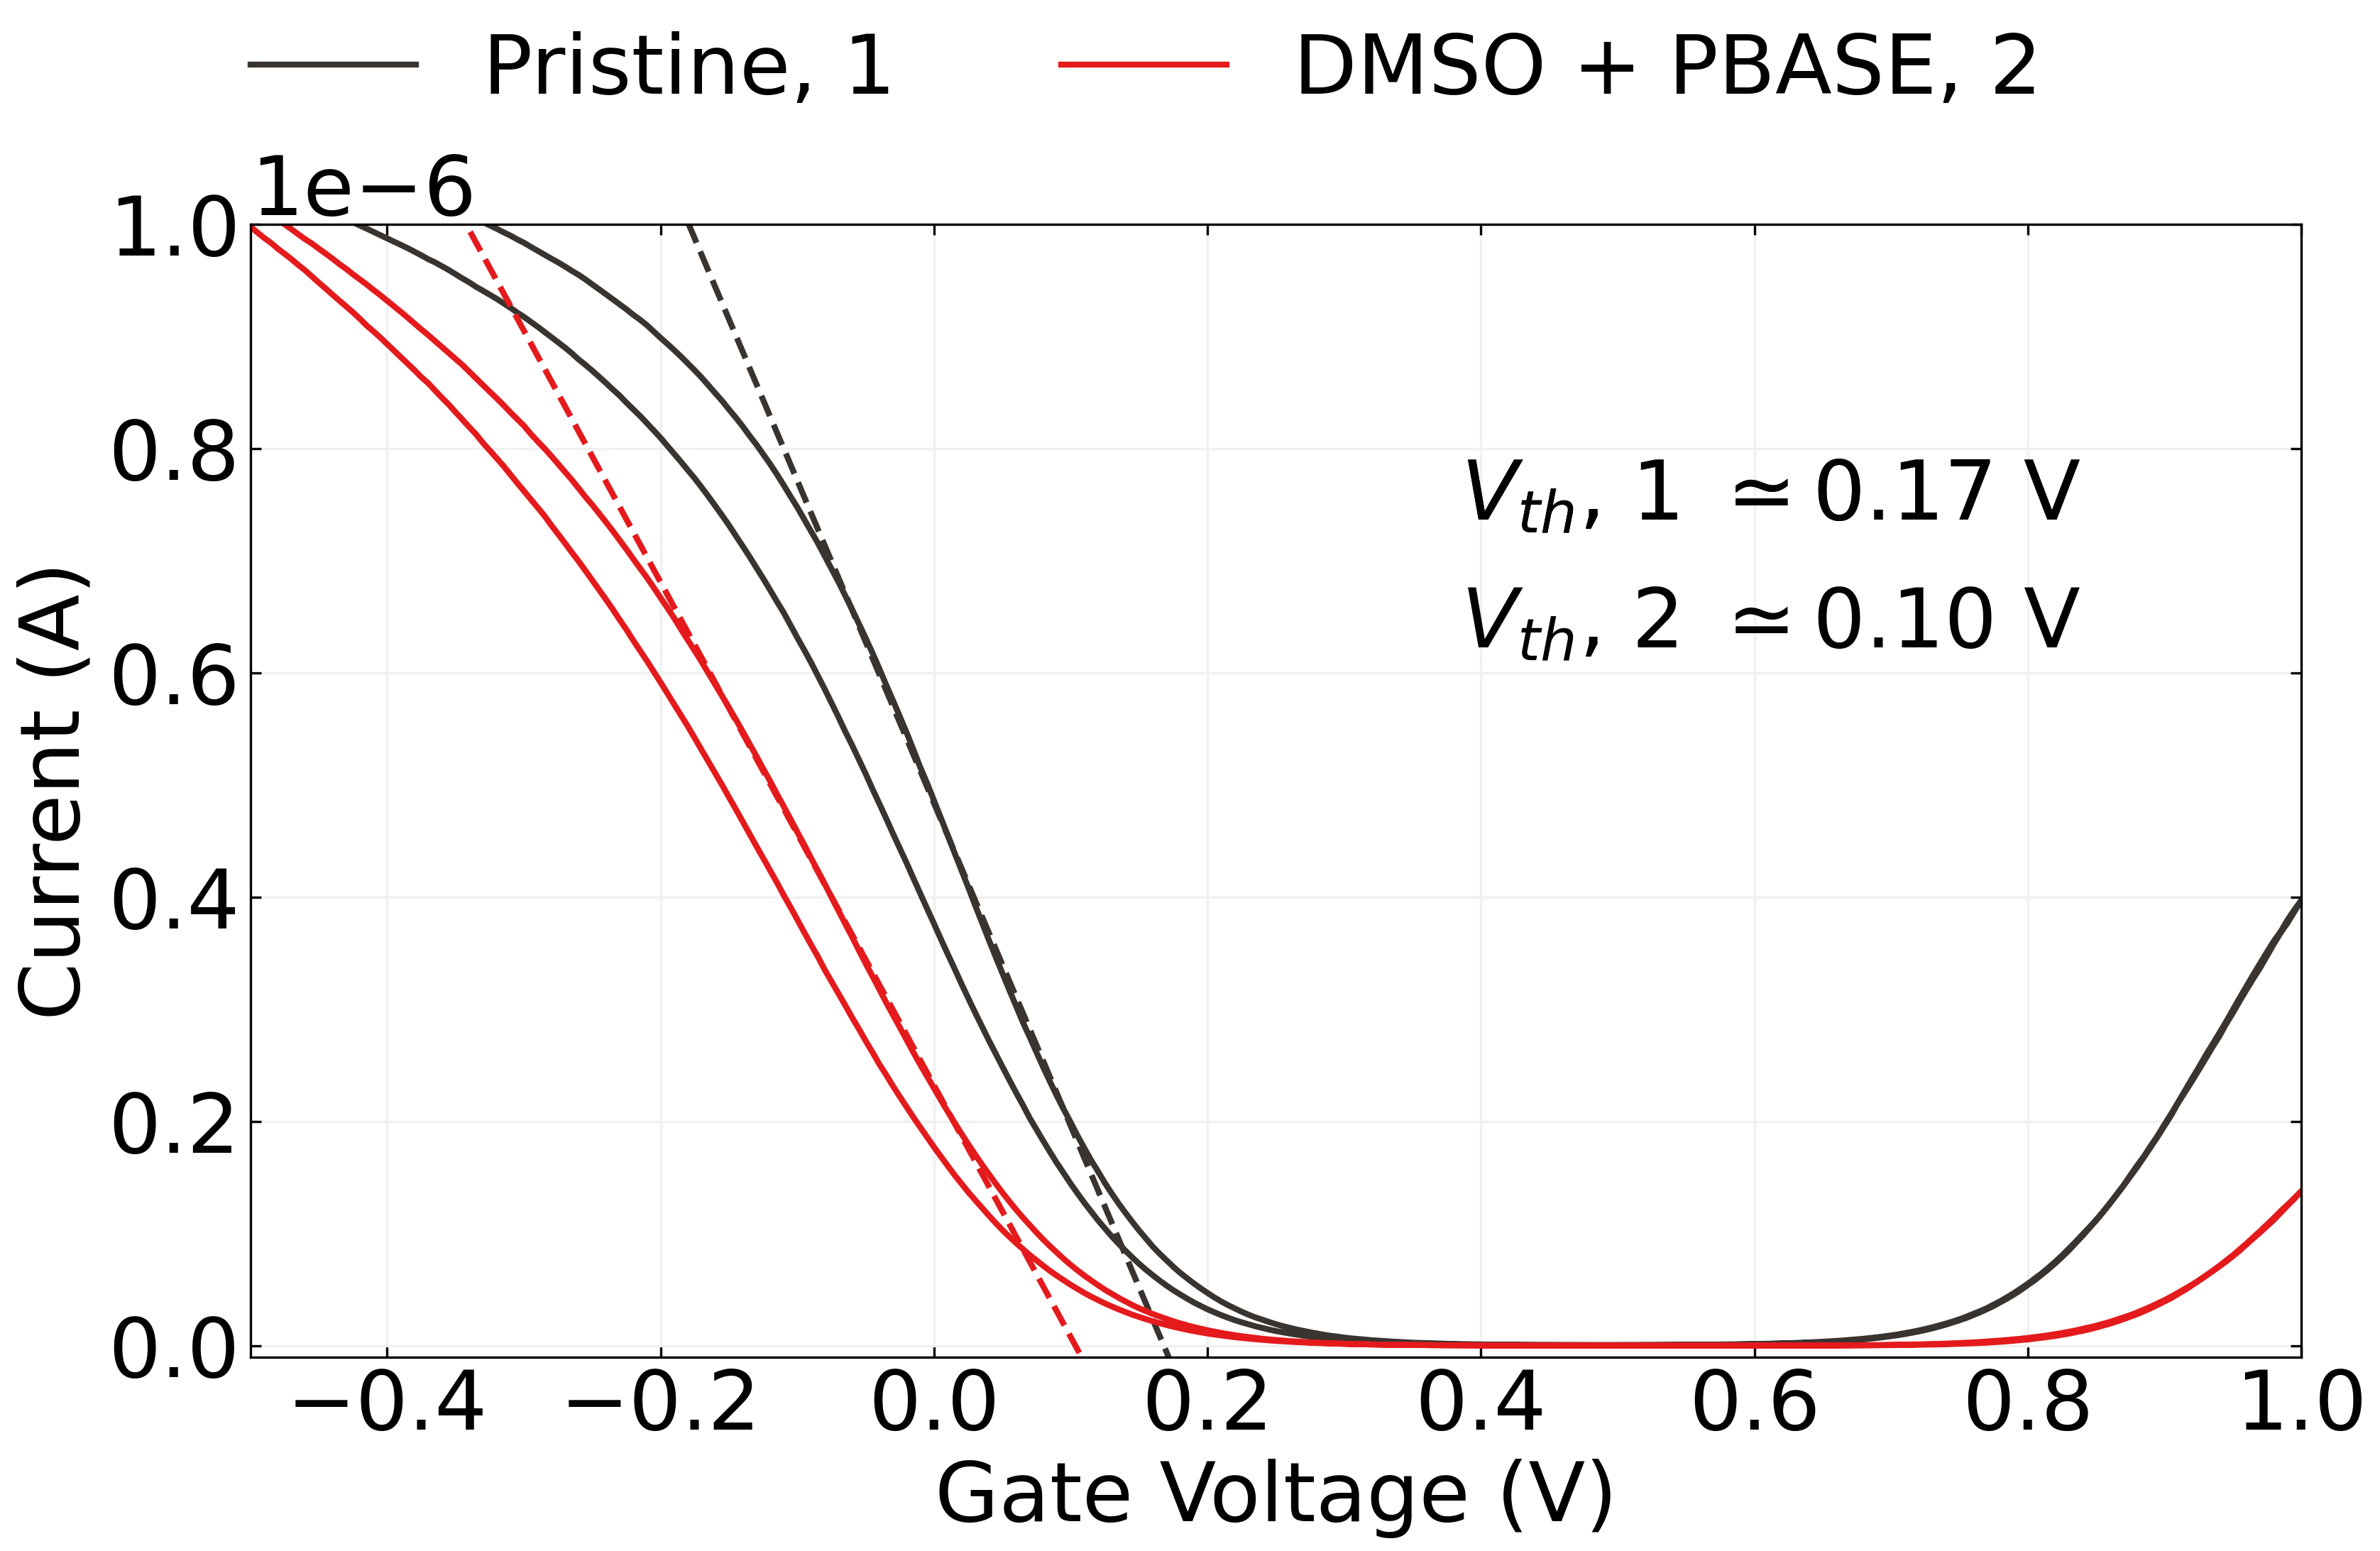
\includegraphics{figures/ch6/Q23D7_ch3_DMSOPBASE.png}

}

}

\end{minipage}%
%
\begin{minipage}[t]{0.01\linewidth}

{\centering 

~

}

\end{minipage}%

\caption{\label{fig-PBASE-vs-solvent-only}The electrical transfer
characteristics of carbon nanotube transistors (\(V_{ds}\) = 100 mV)
before and after being submerged in MeOH (a) or DMSO (b) for one hour
and subsequently rinsed with deionised water. The change in
characteristics of similar transistor channels after being submerged in
these same solvents containing 1 mM PBASE for one hour and then rinsed
are shown in (c) and (d) respectively. Average threshold voltages for
each transfer characteristic curve are also shown (taking the average of
forward and reverse sweep values).}

\end{figure}

Capactive gating results from dense coverage of adsorped molecules on
the carbon nanotube surface which have a low permittivity relative to
the surrounding electrolyte \autocite{Heller2008}. The relative
permittivity of MeOH and DMSO are \(\sim\) 33 \autocite{Mohsen-Nia2010}
and \(\sim\) 47 \autocite{Hunger2010} respectively, which are both much
lower than the relative permittivity of PBS, \(\sim\) 80
\autocite{Shkodra2021}. From Figure~\ref{fig-PBASE-vs-solvent-only} (a)
and Figure~\ref{fig-PBASE-vs-solvent-only} (b), the threshold shift
values found resulting from exposure to each solvent, taking the average
of forward and reverse sweep values from a single device, were
\(\Delta V = -0.15 \pm 0.02\) V and \(\Delta V = -0.15 \pm 0.01\) V for
MeOH and DMSO respectively. The average threshold shift value for a
second device exposed to MeOH was \(\Delta V = -0.16 \pm 0.02\) V,
indicating that this threshold shift result is reproducible.

Using the same characterisation process as in this work, Murugathas
\emph{et al.} \autocite{Murugathas2019a} showed that the attachment of
PBASE to a solvent-deposited carbon nanotube network had little effect
on channel threshold voltage, implying the presence of PBASE had not
significantly influenced channel gating. Here, an average threshold
voltage shift of \(-0.06\pm0.04\) V is seen after PBASE
functionalisation in MeOH and \(-0.06\pm0.01\) V after PBASE
functionalisation in DMSO. These threshold voltage shifts are small
compared to solvent only. It is possible that the attachment of PBASE
prevents solvent adsorption, and has a small negative gating effect on
the channel. Alternatively, while the solvent negatively gates the
channel, resulting in a threshold shift of -0.15 V, the PBASE may be
counteracting this by positively gating the channel, resulting in a
threshold shift of +0.09 V. Murugathas \emph{et al.} also observed a
slight increase in channel conductance after PBASE functionalisation
\autocite{Murugathas2019a}. Figure~\ref{fig-PBASE-vs-solvent-only} also
shows a slight increase in channel conductance post-functionalisation in
both Figure~\ref{fig-PBASE-vs-solvent-only} (c) and
Figure~\ref{fig-PBASE-vs-solvent-only} (d) relative to the solvent-only
case in Figure~\ref{fig-PBASE-vs-solvent-only} (a) and
Figure~\ref{fig-PBASE-vs-solvent-only} (b). This result implies that the
presence of PBASE molecules increases channel mobility and therefore
conductance \autocite{Heller2008}.

The absorption of organic solvent by the carbon nanotube network has
unknown but potentially negative implications for biosensor
functionalisation. Use of organic solvents in functionalisation can also
attack the encapsulation layer of devices, promoting gate current
leakage. In light of these issues, recent work has begun to explore
alternative aqueous-based methods for functionalisation of biosensors
\autocite{Khan2021}. The discussion here also illustrates the importance
of considering each substance used when electrical characterising a
device to verify if functionalisation has worked. The qualitative
presence of a change in characteristics (or lack of one) over the full
process is not sufficient to make conclusive remarks regarding
successful functionalisation. A full set of electrical control
measurements are required for an understanding of electronic changes
occuring during the functionalisation process, in the manner of Besteman
\emph{et al.} \autocite{Besteman2003}.

\hypertarget{sec-PBA}{%
\section{Attachment of 1-Pyrenebutyric Acid}\label{sec-PBA}}

\hypertarget{comparing-attachment-methods}{%
\subsection{Comparing Attachment
Methods}\label{comparing-attachment-methods}}

Another linker molecule that can be used to attach receptor molecules to
a carbon nanotube or graphene channel is 1-pyrenebutyric acid (PBA or
PyBA). As with PBASE, the pyrene group of PBA has a \(\pi\) interaction
with the carbon rings of the channel surface. It is possible to react
PBA with 1-ethyl-3-(3-dimethylaminopropyl) carbodiimide hydrochloride
(EDC or EDAC) to form an \emph{O}-acylisourea intermediate, which can
then react with an amine group on a biomolecule and form an amide bond
\autocite{Sehgal1994,Hermanson2013-4}. The water solubility of EDC means
that, unlike PBASE, it is possible to functionalise with EDC dissolved
in water rather than in an organic solvent. However, like PBASE, EDC and
the \emph{O}-acylisourea intermediate are prone to hydrolysis,
especially in acidic conditions.

\newpage
\thispagestyle{empty}
\KOMAoptions{paper=landscape,pagesize}

\hfill\break
\hfill\break

\hypertarget{tbl-pba-functionalisation}{}
\begin{longtable}[]{@{}llllllll@{}}
\caption{\label{tbl-pba-functionalisation}Comparison of 1-pyrenebutyric
acid (PBA) functionalisation processes used for immobilisation of
proteins, enzymes and aptamers onto carbon nanotubes and graphene.
1-ethyl-3-(3-dimethylaminopropyl) carbodiimide hydrochloride (EDC) and
NHS were co-mingled in PBS or DI water in each process - some papers
used N-hydroxysulfosuccinimide instead of N-hydroxysuccinimide, and both
compounds are abbreviated as NHS in this table for simplicity. Device
exposure times to each solution are shown next to the solution
concentration. Blank entries indicate there was no mention of the
parameter in a particular paper. \(^†\)PEG or PEG pyrene were used to
reduce non-specific binding. \(^{††}\)Several pyrene-based linkers were
compared and PBA gave an optimal functionalisation
result.}\tabularnewline
\toprule\noalign{}
Solvent & Channel & PBA (mM) & Time (hr) & EDC (mM) & NHS (mM) & Time
(min) & References \\
\midrule\noalign{}
\endfirsthead
\toprule\noalign{}
Solvent & Channel & PBA (mM) & Time (hr) & EDC (mM) & NHS (mM) & Time
(min) & References \\
\midrule\noalign{}
\endhead
\bottomrule\noalign{}
\endlastfoot
DMF & Graphene & 0.6 & 1 & - & - & 120 & Gao, 2016\(^†\).
\cite{Gao2016} \\
& & 5 & 2 & 2 & 5 & 30 & Mishyn, 2022. \cite{Mishyn2022} \\
& CNT & 100 & 3 & 200 & - & 30 & Min, 2012. \cite{Min2012} \\
& Graphene, CNT & 7.6 & 2 & 8 & 20 & 120 & Xu, 2014. \cite{Xu2014} \\
DI water & CNT & - & - & 32 & 12 & Overnight & Pacios, 2012\(^†\).
\cite{Pacios2012} \\
Ethanol & CNT & 1 & 1 & 100 & 100 & 20 & Filipiak, 2018\(^†\).
\cite{Filipiak2018} \\
Acetonitrile & Graphene & 1 & 1 & 400 & 100 & 60 & Tong, 2020\(^{††}\).
\cite{Tong2020} \\
Borax & CNT & 2 & 24 & 2.5 & - & 1080 & Liu, 2011\(^†\).
\cite{Liu2011} \\
DMSO & Graphene & 5 & 1 & 50 & 50 & 90 & Fenzl, 2017.
\cite{Fenzl2017} \\
\end{longtable}

\newpage
\KOMAoptions{paper=portrait,pagesize}

Therefore, like PBASE, it should be stored at −20°C, and warmed to room
temperature to prevent condensation build-up, since exposure to
condensation will hydrolyse the reagent \autocite{Hermanson2013-4}.
Furthermore, by adding N-Hydroxysuccinimide (NHS) or
N-hydroxysulfosuccinimide (sulfo-NHS) to the reaction vessel, PBASE is
formed as an active intermediate, which is less prone to hydrolysis and
increases the PBA/EDC reaction yield
\autocite{Sehgal1994,Hermanson2013-4,Hermanson2013-14}.

A full comparison of functionalisation procedures used for linking
carbon nanotube and graphene devices to aptamers and proteins with PBA
is given in Table~\ref{tbl-pba-functionalisation}. To the best of my
knowledge, this table is as complete a summary as possible of
1-pyrenebutyric acid functionalisation processes for carbon nanotube and
graphene field-effect transistor biochemical sensors. By comparing
Table~\ref{tbl-pbase-functionalisation} and
Table~\ref{tbl-pba-functionalisation}, it is clear that PBASE is more
widely used for non-covalent functionalisation than PBA/EDC.

As was the case for PBASE, there are a wide range of process variables
used for the functionalisation process, with little justification used
for variables chosen. Also notable is the frequent use of polyethylene
glycol (PEG) or pyrene-PEG for prevention of non-specific binding (NSB).
Non-specific binding is discussed further in
\textbf{?@sec-non-specific-binding}. Despite being less widely used,
Mishyn \emph{et al.} \autocite{Mishyn2022} state a preference for the
use of PBA/EDC over PBASE, as they found it was less prone to hydrolysis
and gave a larger reaction yield when binding ferrocene to graphene. A
potential downside of using PBA/EDC for protein immobilisation is that
EDC has numerous ways of interacting with proteins, and not all of these
are necessarily desirable. Furthermore, the addition of NHS may also
cause other issues, such as precipitation of the reaction compound
\autocite{Hermanson2013-4}. The greater range of process variables
involved in the functionalisation also adds to the complexity of
reproducing past results.

\hypertarget{raman-spectroscopy}{%
\subsection{Raman Spectroscopy}\label{raman-spectroscopy}}

\begin{figure}

{\centering 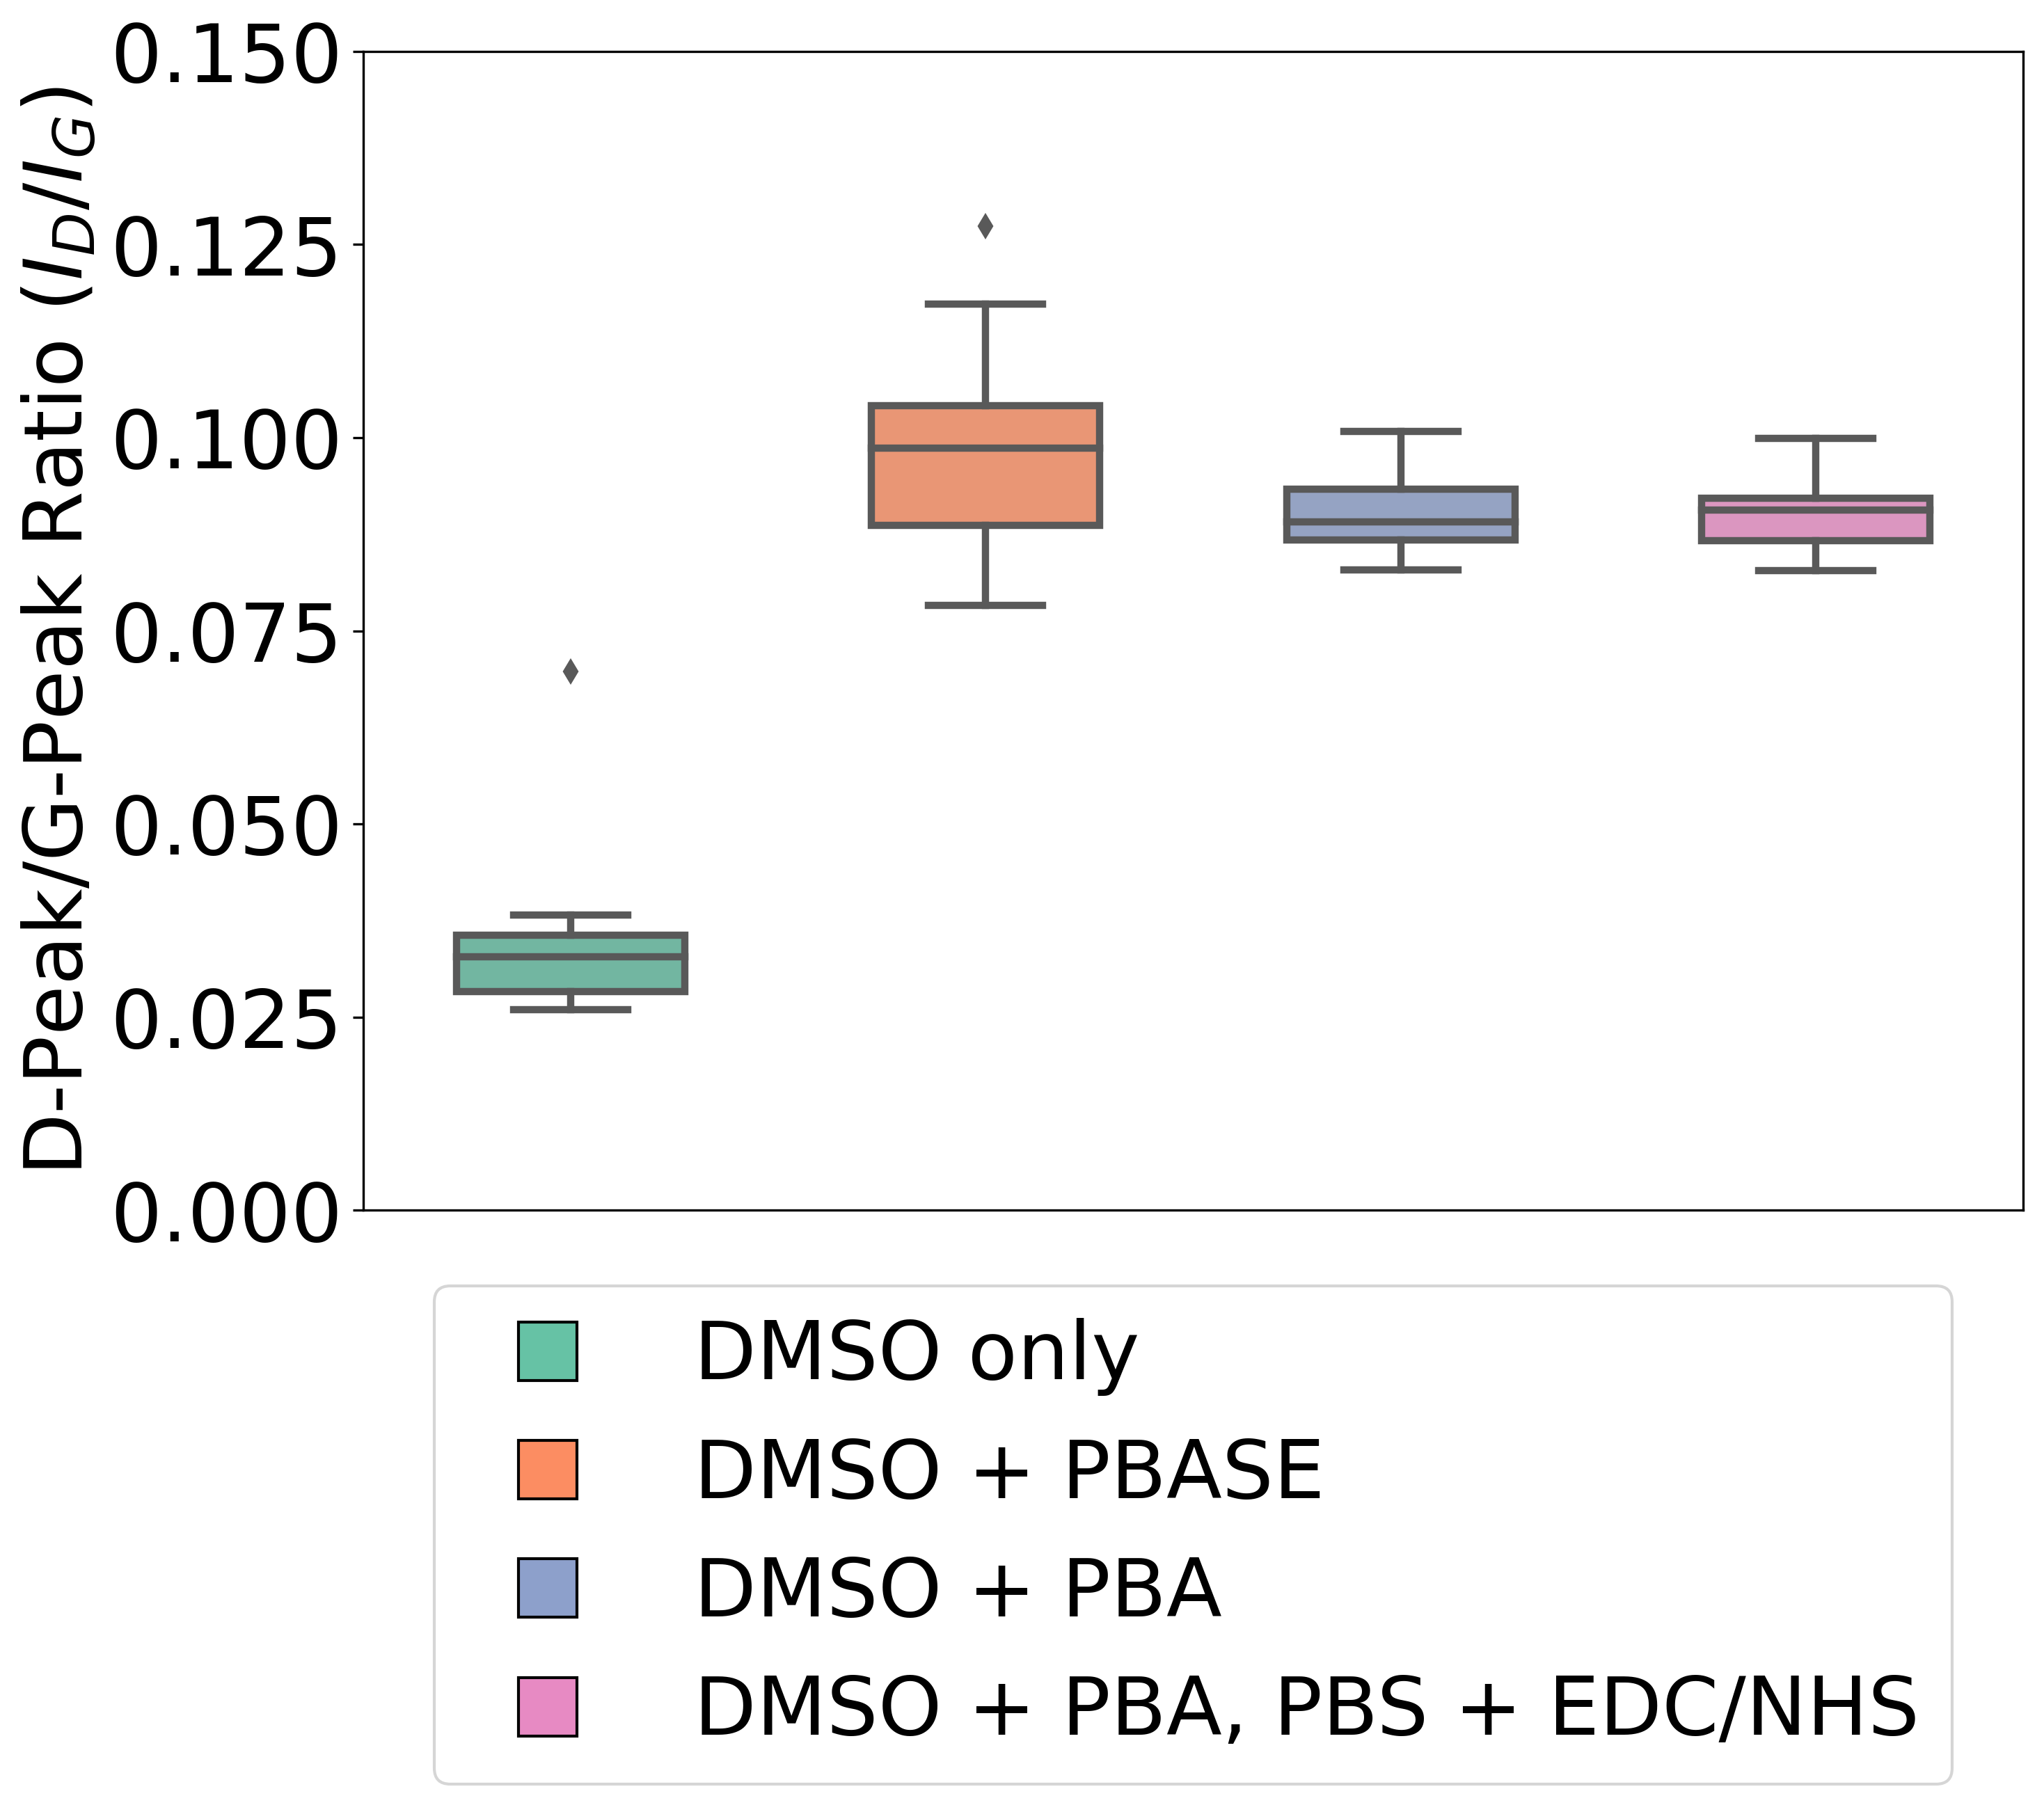
\includegraphics[width=0.5\textwidth,height=\textheight]{figures/ch6/comparison_raman.png}

}

\caption{\label{fig-linker-raman}This box plot shows the distribution of
D-band peak to G\(^+\)-band peak ratio, \(I_D/I_G\), across nine
locations for a selection of chemically-modified carbon nanotube films.
The D-band and G-band intensities for all samples were first normalised
to the intensity peak corresponding to the SiO\(_2\) substrate.}

\end{figure}

Raman spectroscopy was used to verify the attachment of PBA to a carbon
nanotube network film with a SiO\(_2\) substrate in the manner outlined
in \textbf{?@sec-raman-characterisation}. As highly-bundled devices were
found to have less defects present prior to modification, as discussed
in \textbf{?@sec-pristine-raman}, solvent-deposited films were used for
the verification of pyrene attachment to prevent the initial presence of
defects influencing the analysis. Droplets of DMSO solution were placed
on three (solvent-deposited) carbon nanotube films taken from the same
wafer. The DMSO solution on one film contained 5 mM PBA, the solution on
another film contained 5 mM PBASE, and the DMSO on the final film
contained no linker molecule. After incubation for 1 hour, films were
rinsed for 15 s with DMSO, then for 15 s with IPA to remove excess DMSO
while avoiding hydrolysis of the PBASE. After the first set of Raman
spectra was taken, the film initially exposed to PBA was further exposed
to a solution of 20 mM EDC and 40 mM NHS in \(1 \times\) phosphate
buffer saline (PBS) electrolyte for 30 minutes, and a second set of
Raman spectra was taken for this film. As in
\textbf{?@sec-pristine-raman}, two spectra taken at each position were
processed according to Section~\ref{sec-raman-analysis}, and the
SiO\(_2\) reference peak measured in the wavenumber range 100
cm\(^{-1}\) \(-\) 650 cm\(^{-1}\) was used to normalise the D-band and
G-band peaks from the wavenumber range 1300 cm\(^{-1}\) \(-\) 1650
cm\(^{-1}\). The ratio between the average intensity of the D-peak and
the G\(^+\)-peak at each position was calculated, and the distribution
of ratio values corresponding to each modified film is shown in
Figure~\ref{fig-linker-raman}.

There is a \(\sim 3 \times\) increase in the intensity ratio \(I_D/I_G\)
for both the films modified with PBASE and PBA compared to the film
which was only exposed to DMSO. Previous works have found that a change
in the intensity ratio indicates successful \(\pi\)-stacking on the
carbon nanotube surface, as it indicates surface modification of the
carbon nanotubes has occurred \autocite{Wei2010,Lan2013}. Wei \emph{et
al.} \autocite{Wei2010} found functionalisation with PBASE altered the
ratio by a factor of \(\sim 1.5 \times\), while Lan \emph{et al.}
\autocite{Lan2013} found that functionalisation with PBA altered the
ratio by a factor of \(\sim 0.8 \times\). The reason for the large
difference between results is not immediately clear, but may result from
the significant differences in the pristine composition and morphology
of carbon nanotube networks used in each publication, and differences in
the functionalisation method used. Across all scan locations in
Figure~\ref{fig-linker-raman}, the value found for \(I_D/I_G\) is
consistently \(\sim 0.095\) for both PBA and PBASE. Furthermore,
subsequent Raman measurements of the PBA-modified film after further
functionalisation with EDC/NHS do not show a significant change in
\(I_D/I_G\). These results indicate that presence of the NHS ester has
little effect on the Raman shift. Raman spectroscopy therefore cannot be
used to distinguish between the presence of PBA and PBASE on the device
surface. However, it is clear that functionalisation of the carbon
nanotube network with both the PBA and PBASE has led to measurable
\(pi\)-stacking between the network and the pyrene group attached to
each compound.

\hypertarget{sec-PBA-characterisation}{%
\subsection{Electrical
Characterisation}\label{sec-PBA-characterisation}}

\begin{figure}

\begin{minipage}[t]{0.03\linewidth}

{\centering 

\raisebox{-\height}{


\includegraphics{figures/(a).png}

}

}

\end{minipage}%
%
\begin{minipage}[t]{0.01\linewidth}

{\centering 

~

}

\end{minipage}%
%
\begin{minipage}[t]{0.45\linewidth}

{\centering 

\raisebox{-\height}{

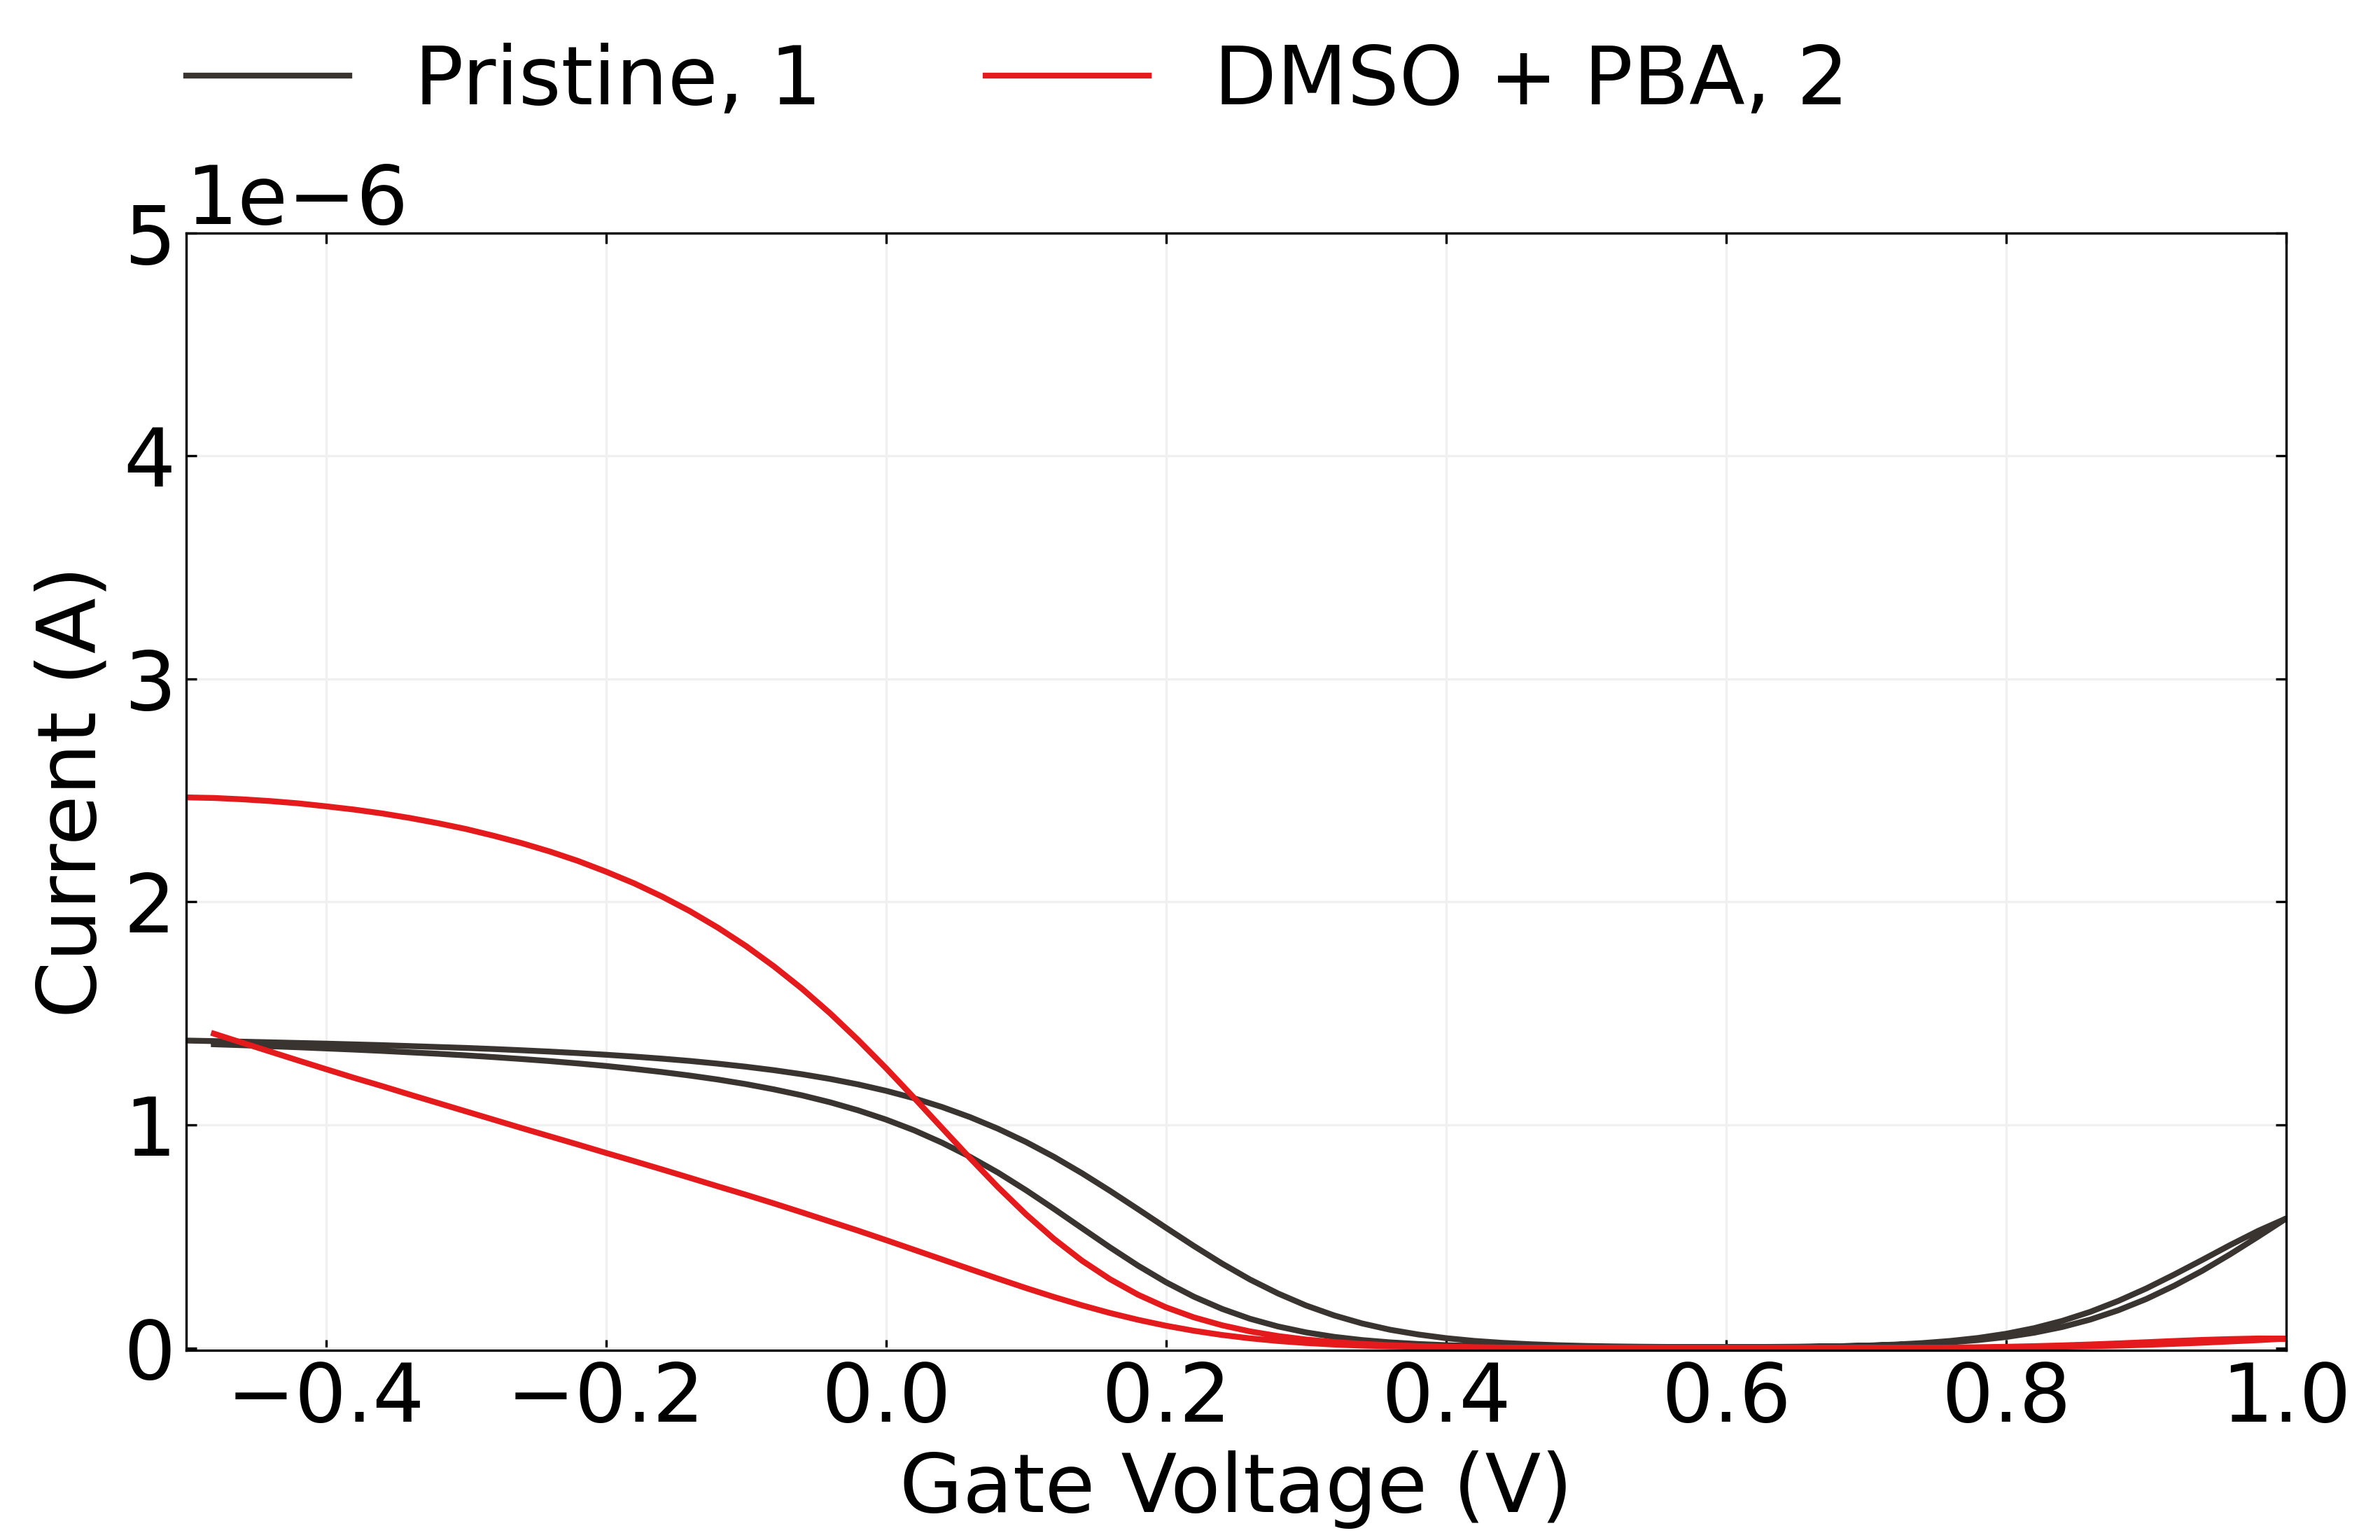
\includegraphics{figures/ch6/NTQ24C10_ch3_comparison_1.png}

}

}

\end{minipage}%
%
\begin{minipage}[t]{0.01\linewidth}

{\centering 

~

}

\end{minipage}%
%
\begin{minipage}[t]{0.03\linewidth}

{\centering 

\raisebox{-\height}{


\includegraphics{figures/(b).png}

}

}

\end{minipage}%
%
\begin{minipage}[t]{0.01\linewidth}

{\centering 

~

}

\end{minipage}%
%
\begin{minipage}[t]{0.45\linewidth}

{\centering 

\raisebox{-\height}{

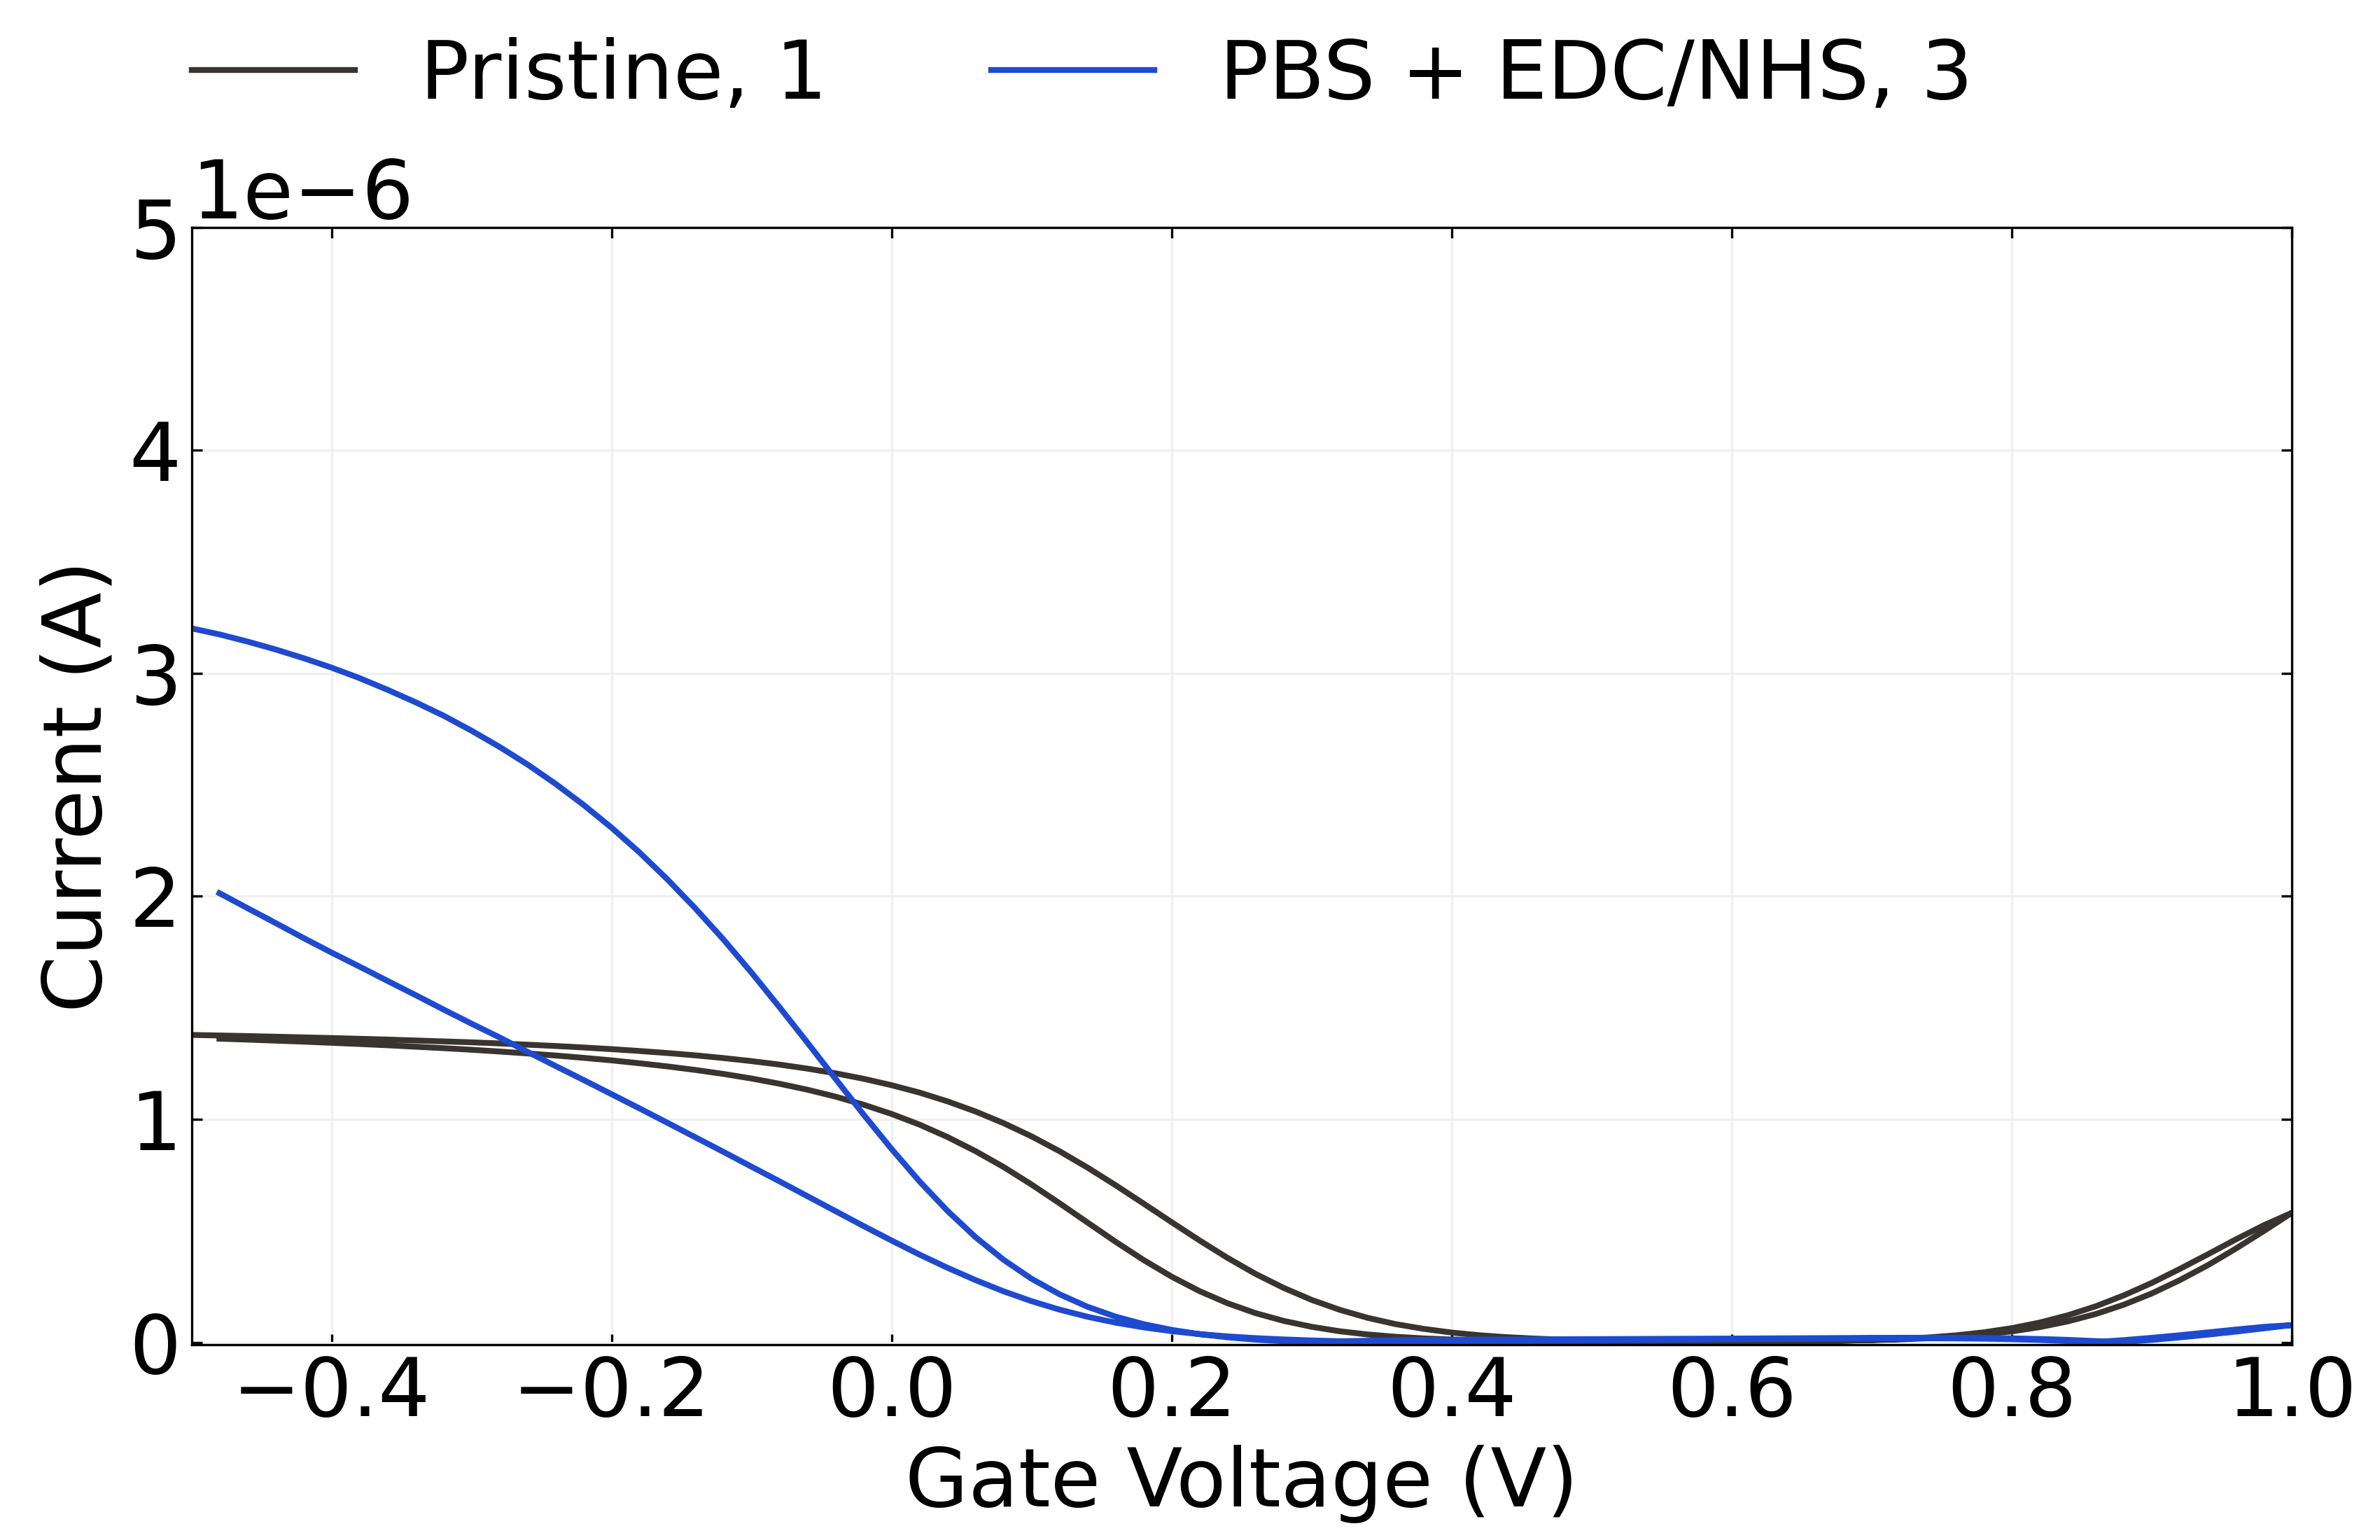
\includegraphics{figures/ch6/NTQ24C10_ch3_comparison_2.png}

}

}

\end{minipage}%
%
\begin{minipage}[t]{0.01\linewidth}

{\centering 

~

}

\end{minipage}%
\newline
\begin{minipage}[t]{0.03\linewidth}

{\centering 

\raisebox{-\height}{


\includegraphics{figures/(c).png}

}

}

\end{minipage}%
%
\begin{minipage}[t]{0.01\linewidth}

{\centering 

~

}

\end{minipage}%
%
\begin{minipage}[t]{0.45\linewidth}

{\centering 

\raisebox{-\height}{

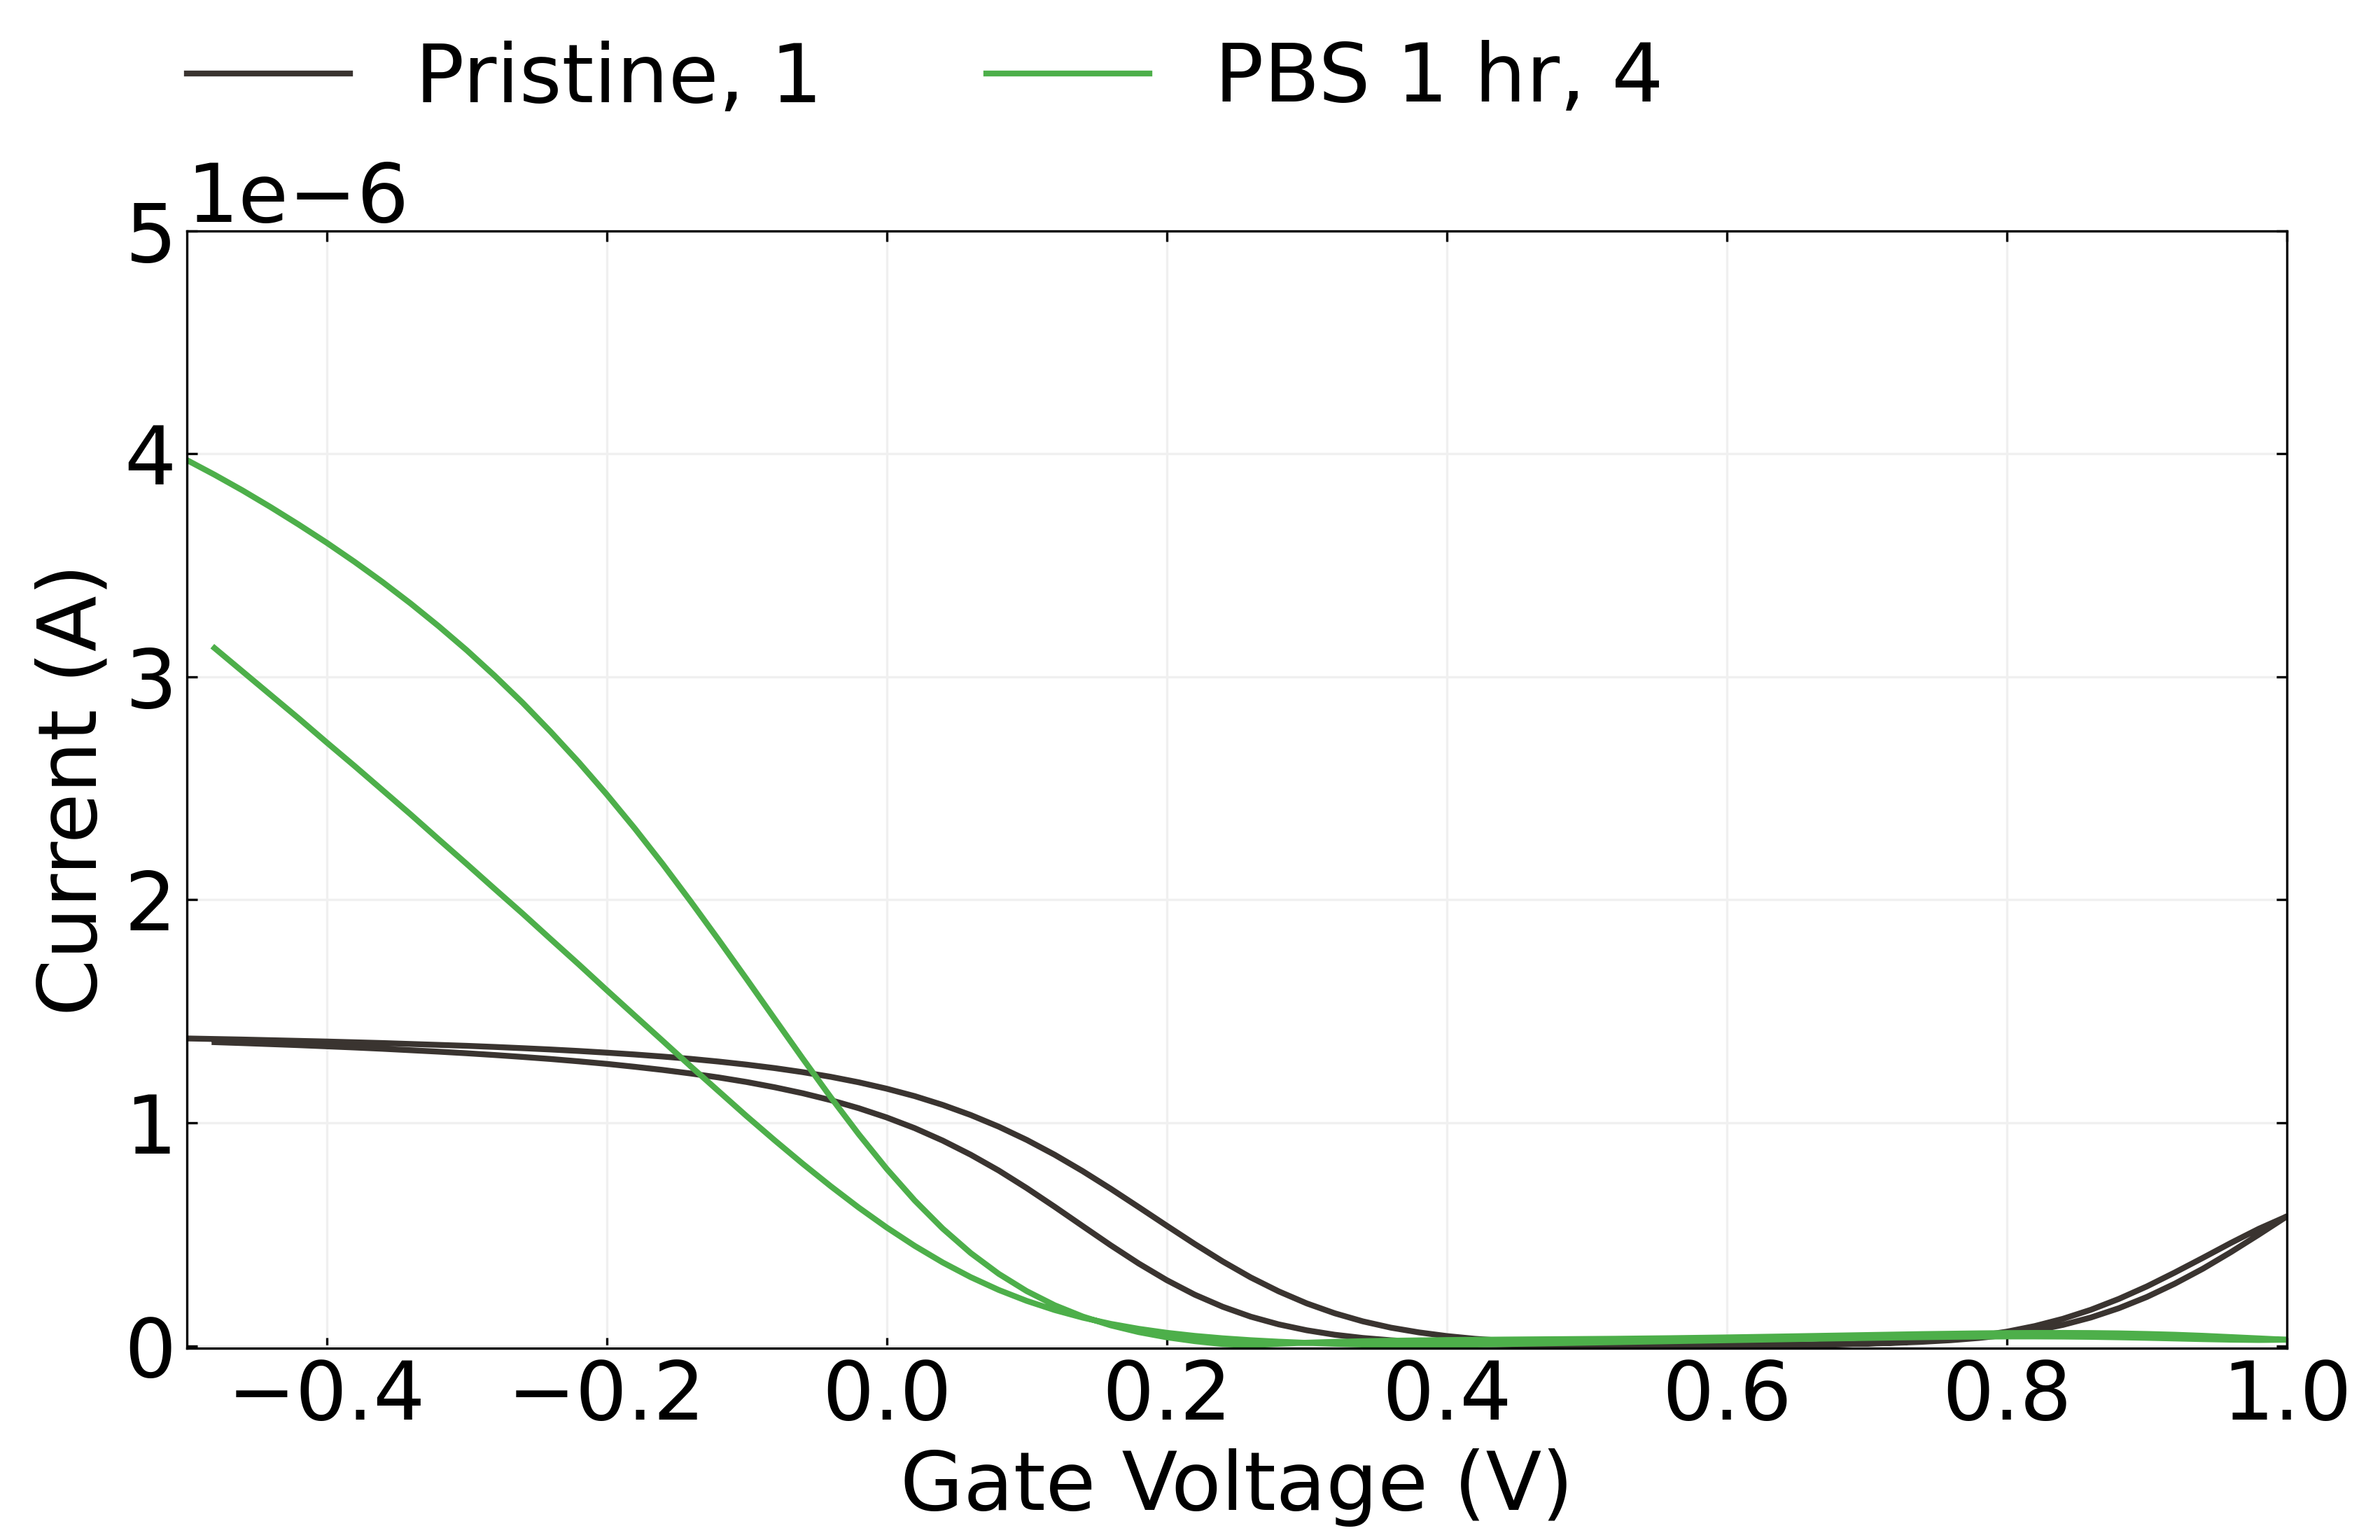
\includegraphics{figures/ch6/NTQ24C10_ch3_comparison_3.png}

}

}

\end{minipage}%
%
\begin{minipage}[t]{0.01\linewidth}

{\centering 

~

}

\end{minipage}%
%
\begin{minipage}[t]{0.03\linewidth}

{\centering 

\raisebox{-\height}{


\includegraphics{figures/(d).png}

}

}

\end{minipage}%
%
\begin{minipage}[t]{0.01\linewidth}

{\centering 

~

}

\end{minipage}%
%
\begin{minipage}[t]{0.45\linewidth}

{\centering 

\raisebox{-\height}{

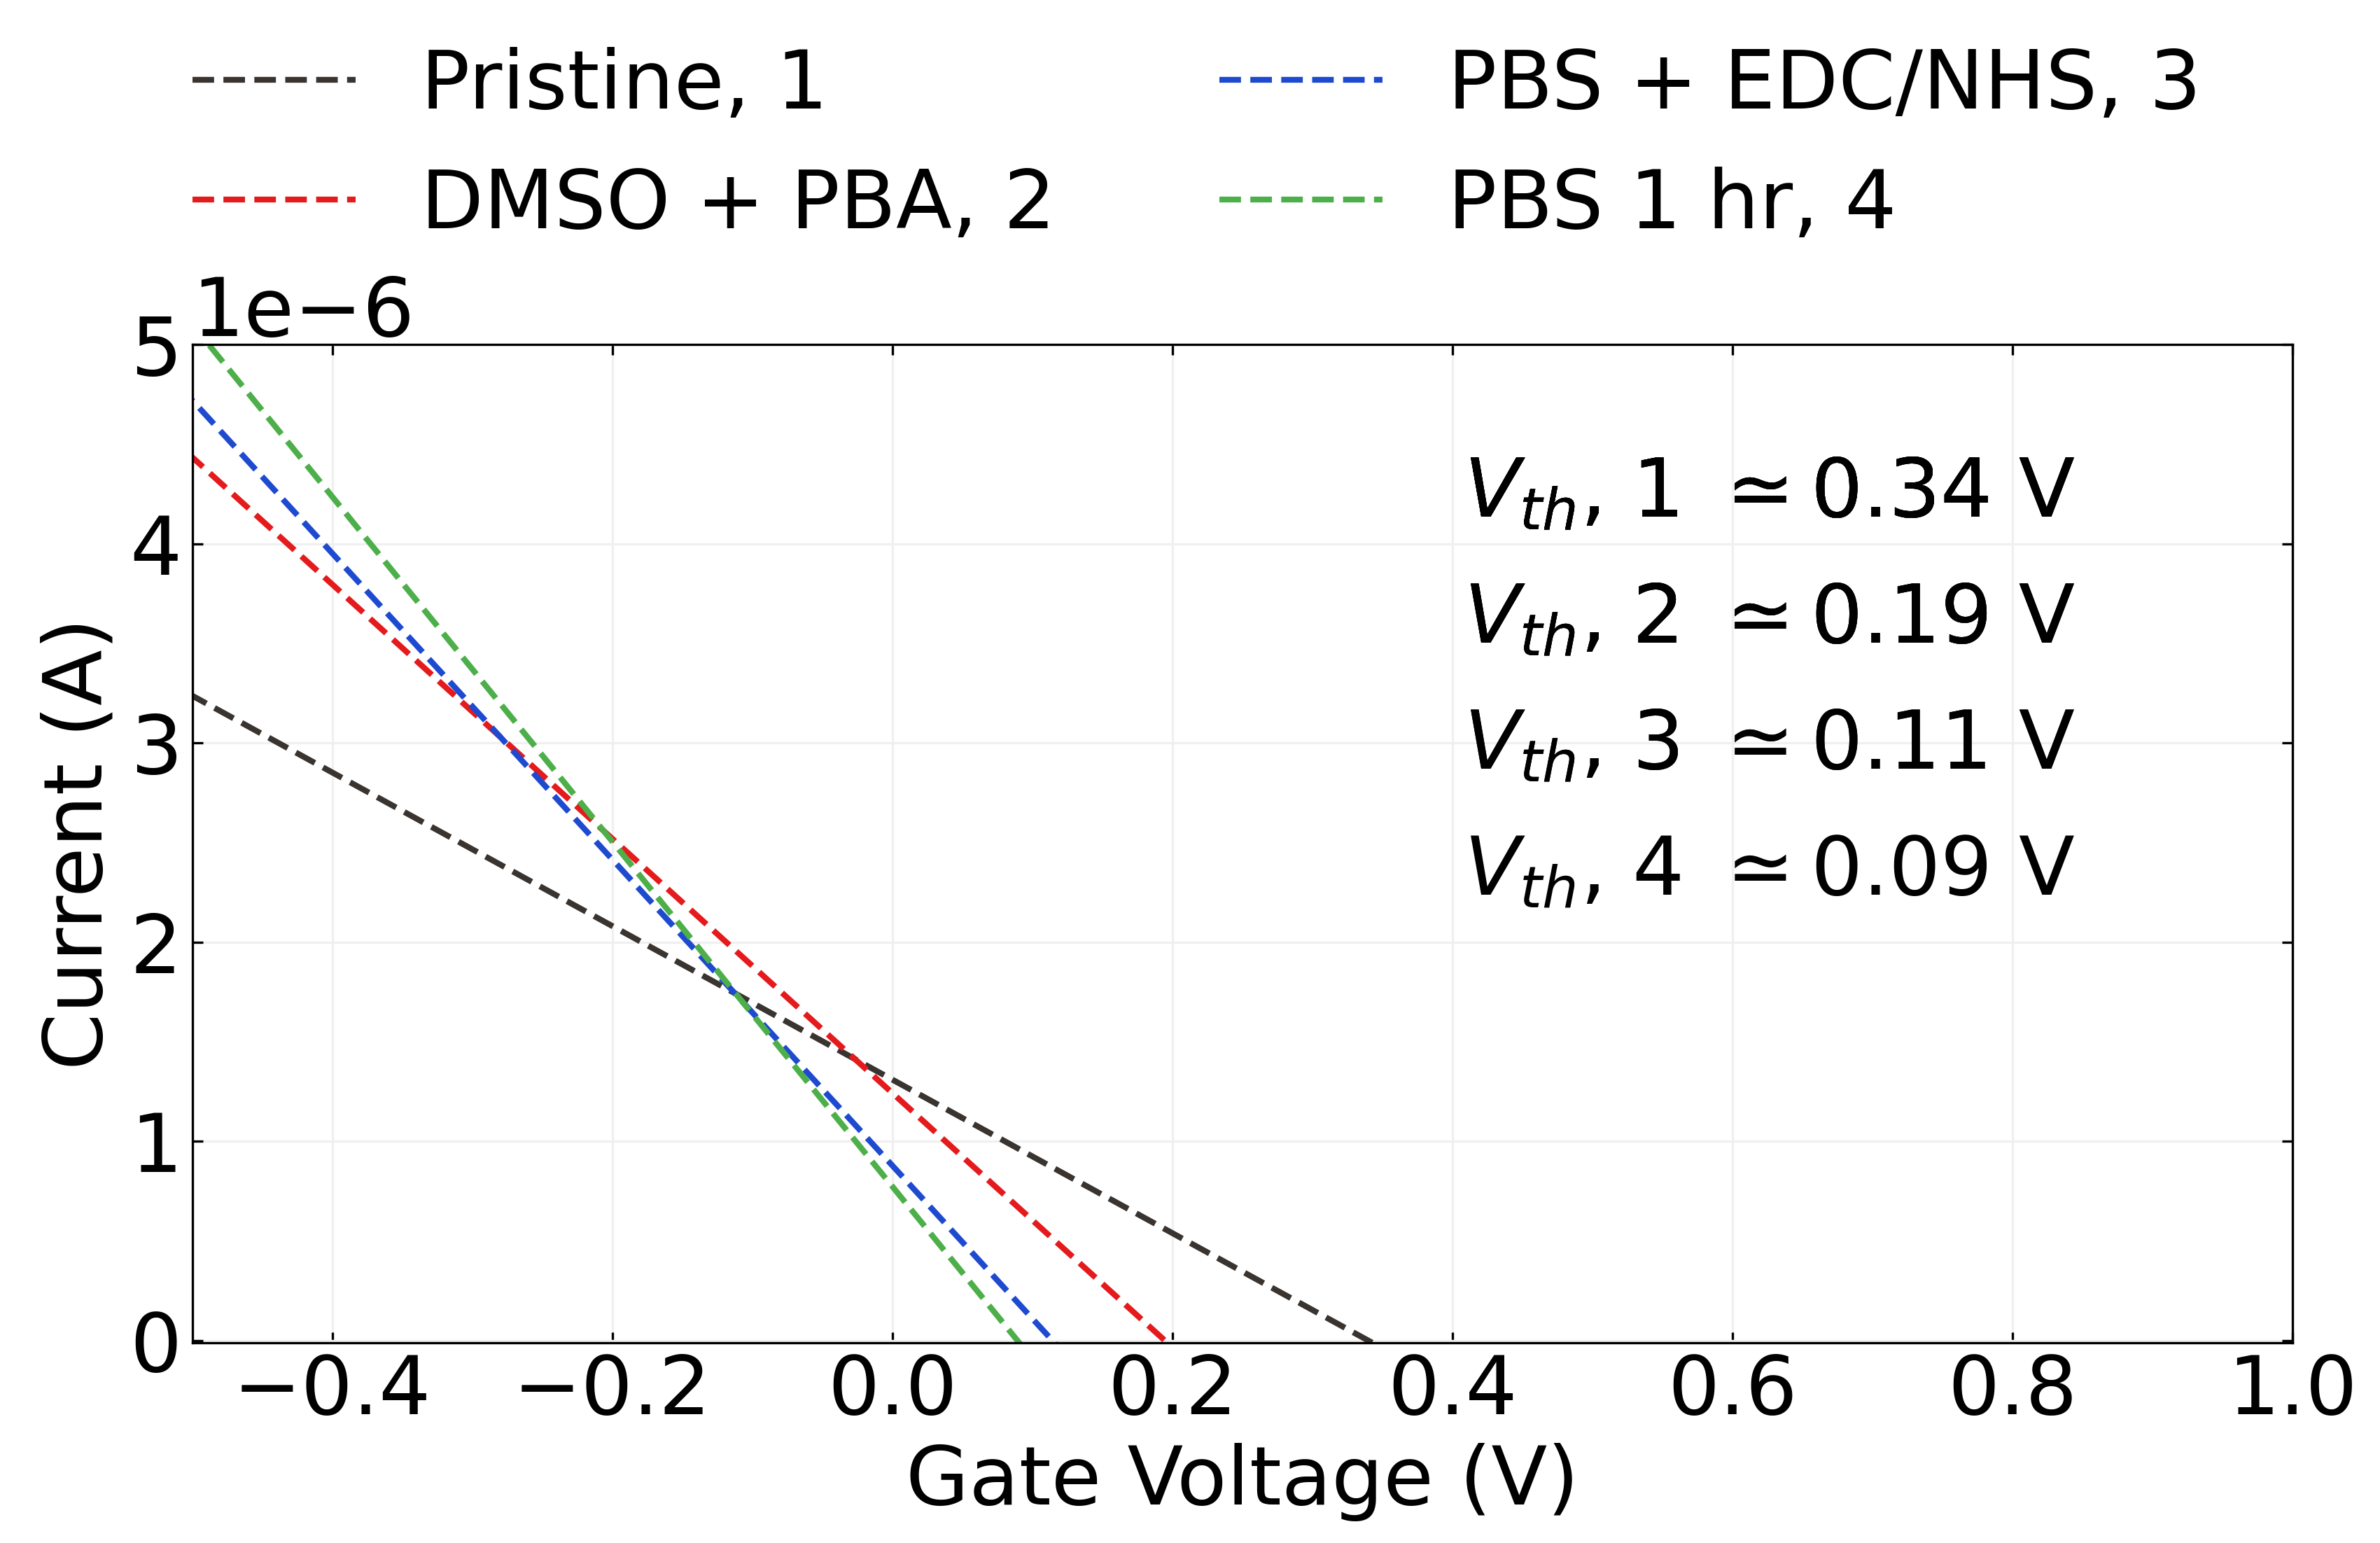
\includegraphics{figures/ch6/NTQ24C10_ch3_comparison_4.png}

}

}

\end{minipage}%
%
\begin{minipage}[t]{0.01\linewidth}

{\centering 

~

}

\end{minipage}%

\caption{\label{fig-pba-functionalisation-threshold-shift}Electrical
transfer characteristics of a carbon nanotube transistor before
functionalisation alongside the transfer characteristics (a) after being
submerged in DMSO with 5 mM PBA in red, (b) after being submerged in PBS
with 20 mM EDC and 40 mM NHS in blue, and (c) after being submerged in
fresh PBS in green. The dashed lines in (d) are linear fits to the
subthreshold slope of each curve, and are shown alongside the threshold
voltages corresponding to each fit.}

\end{figure}

Figure~\ref{fig-pba-functionalisation-threshold-shift} shows the
transfer characteristics of a carbon nanotube transistor channel at
various stages of a PBA/EDC functionalisation, where a excess of
N-hydroxysuccinimide (NHS) was added alongside EDC. A solvent-deposited
carbon nanotube film was used for the device. The PBA was dissolved in
DMSO, and the device channels were exposed to this solution for 1 hour.
The electrical change resulting from PBA exposure is shown in
Figure~\ref{fig-pba-functionalisation-threshold-shift} (a). The
threshold shift with the addition of 5 mM PBA in DMSO for 1 hour is
equivalent to the shift seen when only DMSO is added, \(\Delta V\) =
-0.15 V. The lack of a significant threshold shift attributable to the
PBA is a result of pyrene having a neutral charge state. Any
contributions from the charged carboxyl group are screened from the
carbon nanotube sidewalls by surrounding water molecules
\autocite{Lerner2012}. However, as in the case of the addition of PBASE,
there also appears to be an increase in hole mobility, which may be due
to the pyrene groups increasing connectivity within the carbon nanotube
network \autocite{Murugathas2019a}.

Subsequently, the device was rinsed with \(1 \times\) PBS and exposed to
20 mM EDC and 40 mM NHS in \(1 \times\) PBS electrolyte for 30 minutes.
Figure~\ref{fig-pba-functionalisation-threshold-shift} (b) shows the
change resulting from subsequent EDC/NHS exposure. When EDC/NHS is
added, a threshold shift of \(\Delta\)V \(\sim\) -0.08 V was observed on
multiple channels. The exposure to EDC/NHS negatively shifts the
transfer characteristic curve, most likely due to the PBA present
reacting to form positively-charged \emph{O}-acylisourea esters and
negatively gating the attached carbon nanotube network
\autocite{Heller2008,Hermanson2013-4}.
Figure~\ref{fig-pba-functionalisation-threshold-shift} (c) shows that
this shift is not significantly affected by further exposure of the
channel to PBS. The lack of a change in gating may imply that hydrolysis
over the course of one hour is insufficient to hydrolyse a significant
proportion of the attached \emph{O}-acylisourea or PBASE back to PBA,
leaving them available for reaction with biomolecule amine groups. A
further test could be performed to see if leaving the device submerged
in water over a longer time period to check if ester hydrolysis
eventually affects threshold voltage in a significant manner, but this
was considered to be outside the scope of this work.

\hypertarget{attachment-of-peglyated-pyrene-based-linkers}{%
\section{Attachment of PEGlyated Pyrene-Based
Linkers}\label{attachment-of-peglyated-pyrene-based-linkers}}

\hypertarget{sec-NTA-biotin-PEG}{%
\subsection{Pyrene-NTA, Pyrene-Biotin and
PEGylation}\label{sec-NTA-biotin-PEG}}

Through chemical coupling/conjugation, it is possible to replace the NHS
ester group on PBASE with other groups that can undergo binding
reactions with proteins. Unlike PBASE, these groups do not suffer the
drawback of being readily hydrolysed. For example, PBASE can be modified
with N\(\alpha\),N\(\alpha\)-Bis(carboxymethyl)-L-lysine hydrate (also
known as N-(5-Amino-1-carboxypentyl)iminodiacetic acid, amine-NTA,
AB-NTA) to produce pyrene-nitrilotriacetic acid. The attached NTA group
is able to chelate with metal ions such as Cu\(^{2+}\) or Ni\(^{2+}\),
which then can then coordinate with polyhistidine-tags attached to a
protein \autocite{Holzinger2011,Fruh2011,Amano2016,Chang2017}. Use of
Cu\(^{2+}\) ions over Ni\(^{2+}\) gives stronger histidine bonding and
less non-specific adsorption \autocite{Chang2017}. Functionalisation
using the NTA-Ni\(^{2+}\) chemistry was successfully used to attach
mammalian odorant receptors to a single carbon nanotube for detection of
eugenol vapour in real-time \autocite{Goldsmith2011}. Pyrene-biotin
(pyrene butanol biotin ester) can also be produced for attaching avidin
or strepavidin \autocite{Holzinger2011}. As avidin and strepavidin are
tetrameric, they can be attached to both pyrene-biotin and biotinylated
avi-tagged proteins simultaneously via strong non-covalent bonding,
therefore linking the transducer and receptor
\autocite{Star2003a,Dundas2013,Hermanson2013-11,Fairhead2015}. As the
presence of his-tags and avi-tags on proteins can be readily controlled,
these methods offer improved specificity and directionality over the
traditional amide bonding seen earlier.

It is also possible to attach biocompatible \autocite{Chen2004}
polyethylene glycol (PEG) chains to a pyrene group and modify them with
reactive groups such as NTA and biotin to attach proteins in the manner
outlined in the previous paragraph
\autocite{Hermanson2013-18,Meran2018}. Once modified with PEG, the
hydrophilicity of the PEG increases the water solubility of pyrene
linkers, making it possible to perform a full functionalisation
procedure exclusively in aqueous solution
\autocite{Chen2004,Hermanson2013-18}. By setting the length of the PEG
chain, the size of the linker molecule can be controlled - selection of
a short chain is important for ensuring attached receptors remain within
the Debye length of the transducer \autocite{Shkodra2021}. Note that PEG
naturally repels proteins and can also bond to carbon nanotubes, and
both behaviours have uncertain implications for successful protein
functionalisation \autocite{Chen2004}. However, functionalisation of
both carbon nanotube and graphene transducers with pyrene-PEG-biotin
(PPB) has previously been used for the successful detection of
streptavidin \autocite{Star2003a,Miki2019}. PEG is also charge neutral,
so its presence is not expected to significantly affect device
characteristics \autocite{Chen2004}.

The PEGlyated linkers used in the following sections were purchased
pre-prepared. Pyrene-PEG-NTA (2 kDa) was purchased from Nanocs, while
pyrene-PEG-FITC (2 kDa, 10 kDa), pyrene-PEG-rhodamine (3.4 kDa),
mPEG-Pyrene (10 kDa) and pyrene-PEG-biotin (10 kDa) were purchased from
Creative PEGworks.

\hypertarget{sec-impediments}{%
\section{Identifying Functionalisation Obstacles using Fluorescence
Microscopy}\label{sec-impediments}}

\hypertarget{sec-fluorescence-remarks}{%
\subsection{General Overview}\label{sec-fluorescence-remarks}}

Various dyes and fluorescent tags were used to investigate approaches
for identifying successful attachment of biomolecules to a carbon
nanotube or graphene surface with fluorescence microscopy. The dyes
included fluorescein isothiocyanate (FITC), Rhodamine B and Cyanine 3
(Cy3). Green fluorescent protein was also used for this testing process.
It is important to note that these dyes and the GFP chromophore all
contain benzene rings which are able to \(\pi\)-stack with carbon rings
to some degree
\autocite{Nakayama-Ratchford2007,Tang2012,Khrenova2019,Qiu2019}.
However, there is also significant variation in the extent to which this
\(\pi\)-stacking occurs, which can be seen by comparing
Figure~\ref{fig-FITC-rhodamine-B} (a) and
Figure~\ref{fig-FITC-rhodamine-B} (b). Here, a clear, specific
interaction is seen between Rhodamine B and graphene, but little
interaction between FITC and graphene is observed, even when a longer
exposure time is used. Whether the addition of pyrene linker groups
these dyes, or dye-modified biomolecules, was therefore investigated in
further detail. This process then led to the identification of multiple
issues that could impede a successful device functionalisation.

Both SU8 and AZ\(^\circledR\) 1518 photoresist fluoresced under a
variety of microscope filters, resulting from light interacting with the
photoactive component present in both resists \autocite{Pai2007}. This
background fluorescence was found to drown out fluorescence from a
dye-functionalised device channel, and so photoresist encapsulated
devices were not used for fluorescence imaging. (Consider a photograph
of a dim outdoor lamp; if the photograph was taken on a starless night,
the light from the lamp would show up clearly, but with the sun out the
light would be very difficult to see regardless of how the photograph
was taken). A different type of encapsulation could potentially be used
to verify linker attachment with fluorescence after a device has been
encapsulated. These alternative encapsulation methods for use with
fluorescence microscopy are discussed in
\textbf{?@sec-future-work-fabrication}.

\begin{figure}

\begin{minipage}[t]{0.03\linewidth}

{\centering 

\raisebox{-\height}{


\includegraphics{figures/(a).png}

}

}

\end{minipage}%
%
\begin{minipage}[t]{0.01\linewidth}

{\centering 

~

}

\end{minipage}%
%
\begin{minipage}[t]{0.45\linewidth}

{\centering 

\raisebox{-\height}{

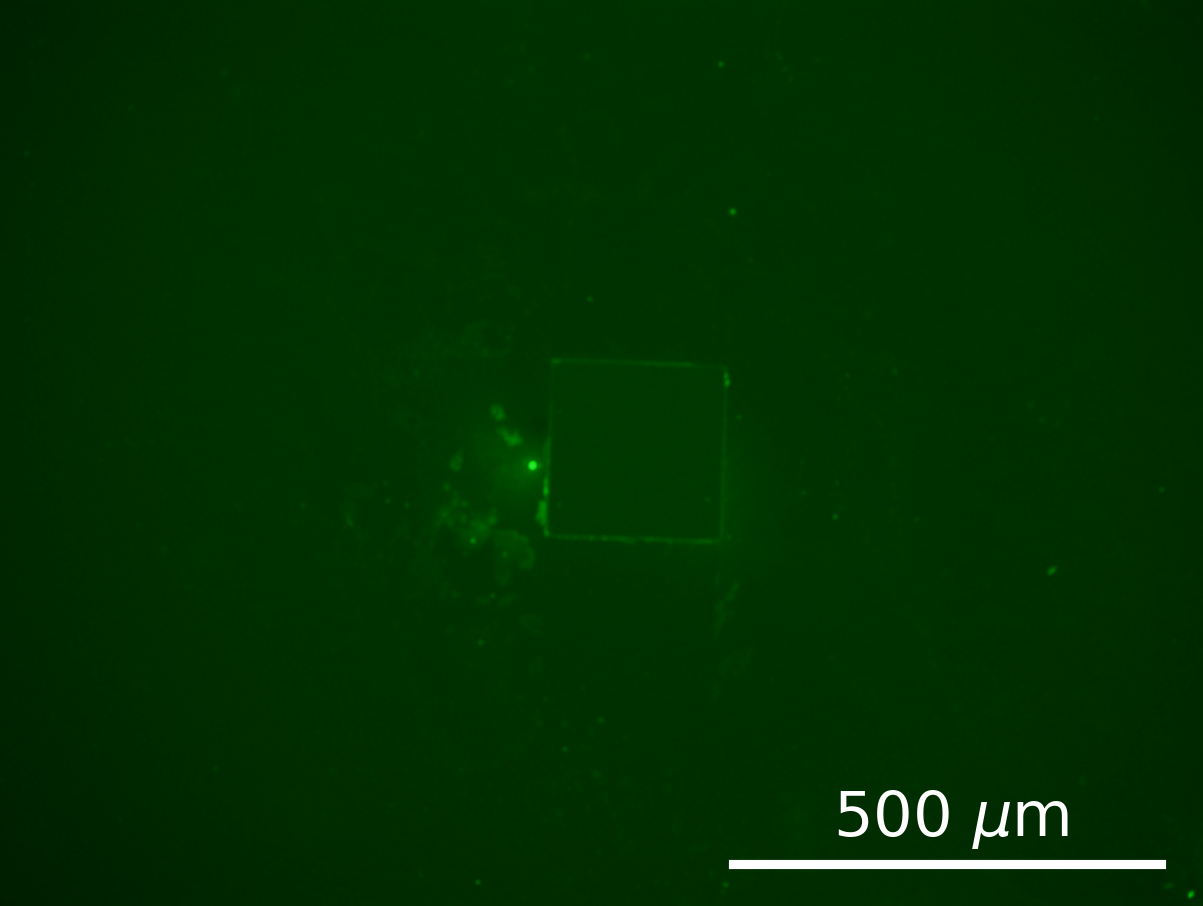
\includegraphics{figures/ch6/NGW8D1_FITC_6.5sexposure_10X_221121.png}

}

}

\end{minipage}%
%
\begin{minipage}[t]{0.01\linewidth}

{\centering 

~

}

\end{minipage}%
%
\begin{minipage}[t]{0.03\linewidth}

{\centering 

\raisebox{-\height}{


\includegraphics{figures/(b).png}

}

}

\end{minipage}%
%
\begin{minipage}[t]{0.01\linewidth}

{\centering 

~

}

\end{minipage}%
%
\begin{minipage}[t]{0.45\linewidth}

{\centering 

\raisebox{-\height}{

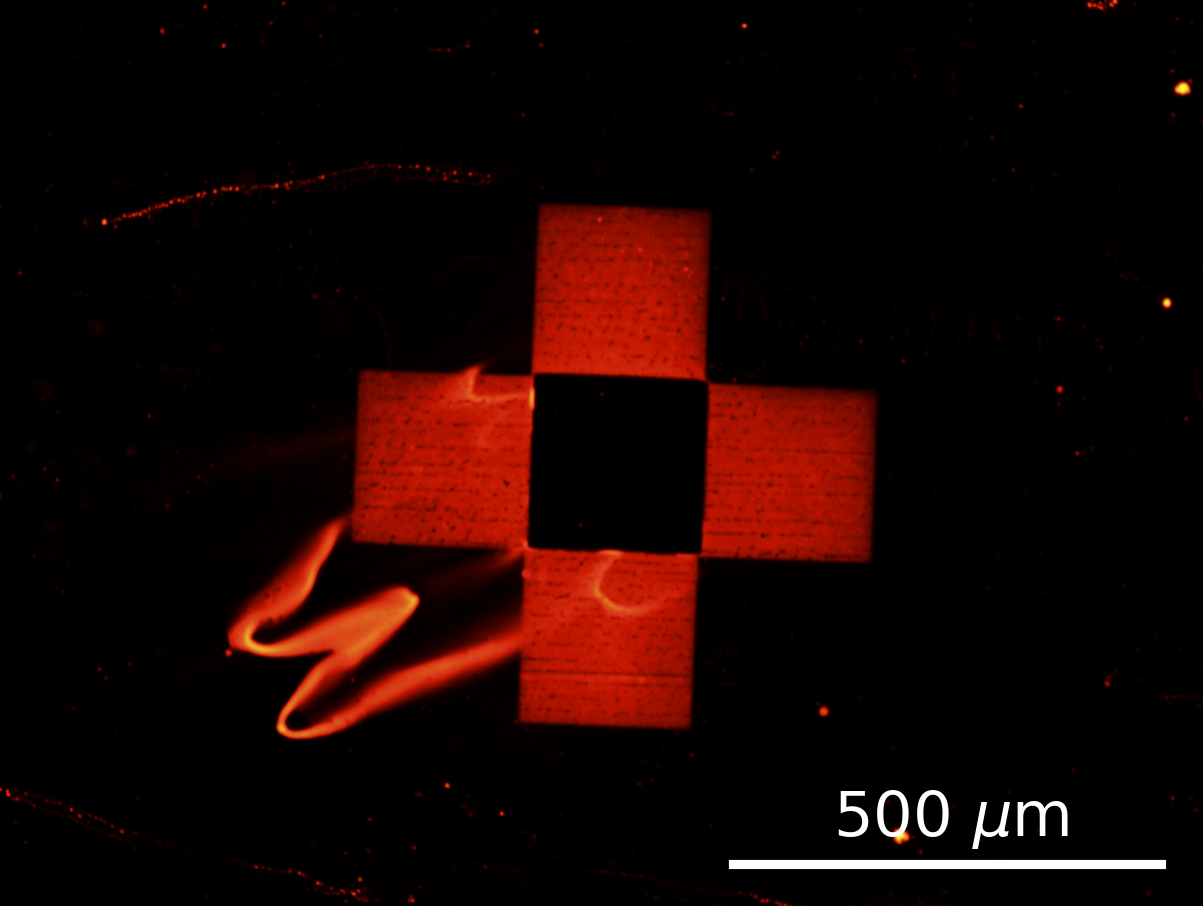
\includegraphics{figures/ch6/NGW8D4_rhodamineB_cornergraphene_221110.png}

}

}

\end{minipage}%
%
\begin{minipage}[t]{0.01\linewidth}

{\centering 

~

}

\end{minipage}%

\caption{\label{fig-FITC-rhodamine-B}Four 200 µm \(\times\) 200 µm
graphene squares modified with the dyes (a) fluorescein isothiocyanate
(FITC) and (b) Rhodamine B. No pyrene/PEG/pyrene-PEG was attached to
these dyes. In (a), an FITC filter and 6.5 s exposure time was used, and
in (b) a Texas Red filter and 1.4 s exposure time was used.}

\end{figure}

\hypertarget{sec-photoresist-contamination}{%
\subsection{Photoresist
Contamination}\label{sec-photoresist-contamination}}

An functionalisation issue quickly encountered when characterising
pyrene-PEG-FITC (PPF) interaction with sensing channels via fluorescence
microscopy was an unwanted secondary interaction between the linker and
residual photoresist. Figure~\ref{fig-photoresist-contamination} (a) and
Figure~\ref{fig-photoresist-contamination} (b) are fluorescence images
of SU8 encapsulation (using the pre-2023 mask) before and after being
exposed to PPF. Despite the same microscope settings being used to take
the images (filter, ISO, contrast, exposure time), the SU8 exposed to
PPF appears much brighter than the pristine SU8. This result indicates
that the linker appears to have an extensive interaction with the
photoresist via an unknown mechanism. No fluorescence is seen from the
device channel. The length of exposure time required to see fluorescence
from the modified channel would lead to fluorescence from the modified
linker attached to the photoresist (as well as the photoresist itself)
flooding the image with light. Therefore, it is not clear whether the
carbon nanotubes have been functionalised with the dye-modified linker.
However, out of caution we can assume that the presence of this
secondary interaction is not desirable.

\begin{figure}

\begin{minipage}[t]{0.03\linewidth}

{\centering 

\raisebox{-\height}{


\includegraphics{figures/(a).png}

}

}

\end{minipage}%
%
\begin{minipage}[t]{0.01\linewidth}

{\centering 

~

}

\end{minipage}%
%
\begin{minipage}[t]{0.45\linewidth}

{\centering 

\raisebox{-\height}{

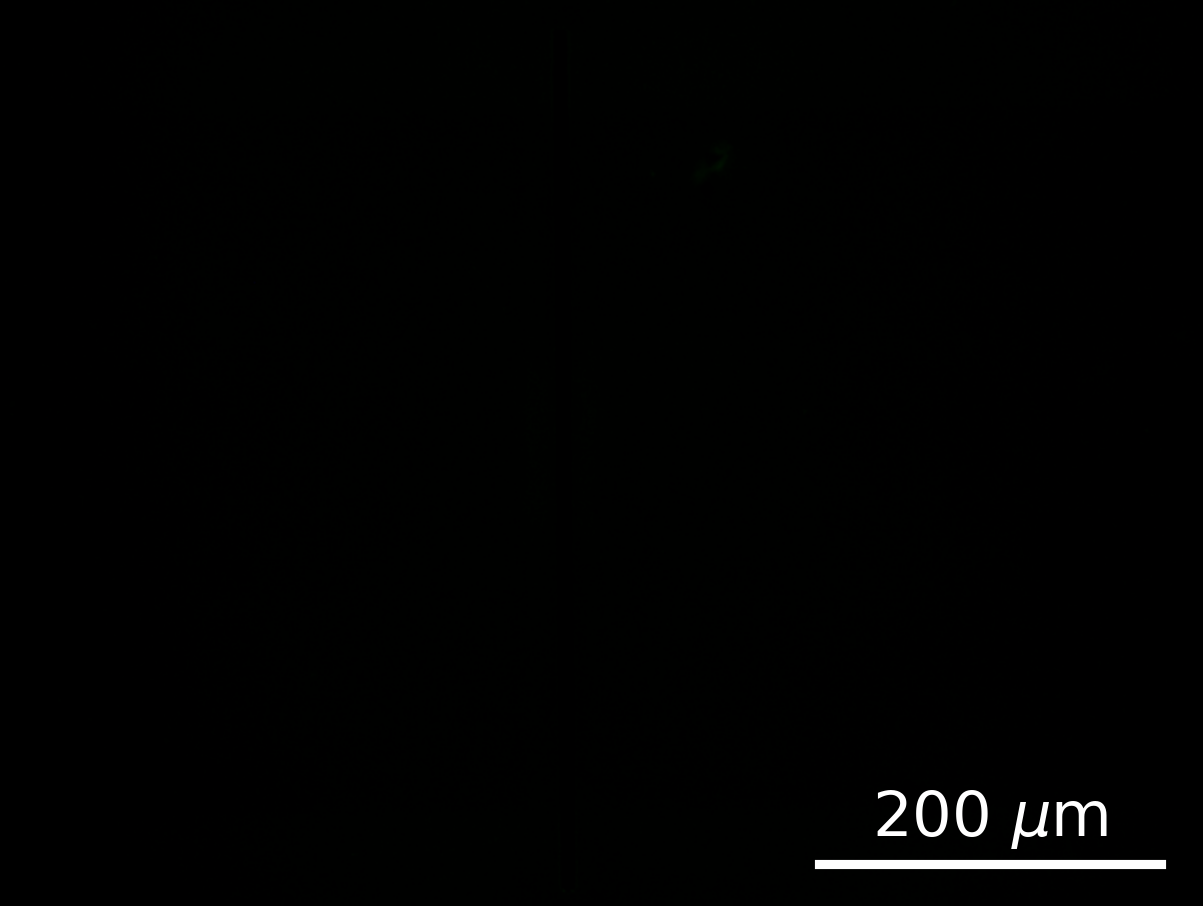
\includegraphics{figures/ch6/modified_SU8only_FITCfilter_channel2_350ms_12.6X_221207.png}

}

}

\end{minipage}%
%
\begin{minipage}[t]{0.01\linewidth}

{\centering 

~

}

\end{minipage}%
%
\begin{minipage}[t]{0.03\linewidth}

{\centering 

\raisebox{-\height}{


\includegraphics{figures/(b).png}

}

}

\end{minipage}%
%
\begin{minipage}[t]{0.01\linewidth}

{\centering 

~

}

\end{minipage}%
%
\begin{minipage}[t]{0.45\linewidth}

{\centering 

\raisebox{-\height}{

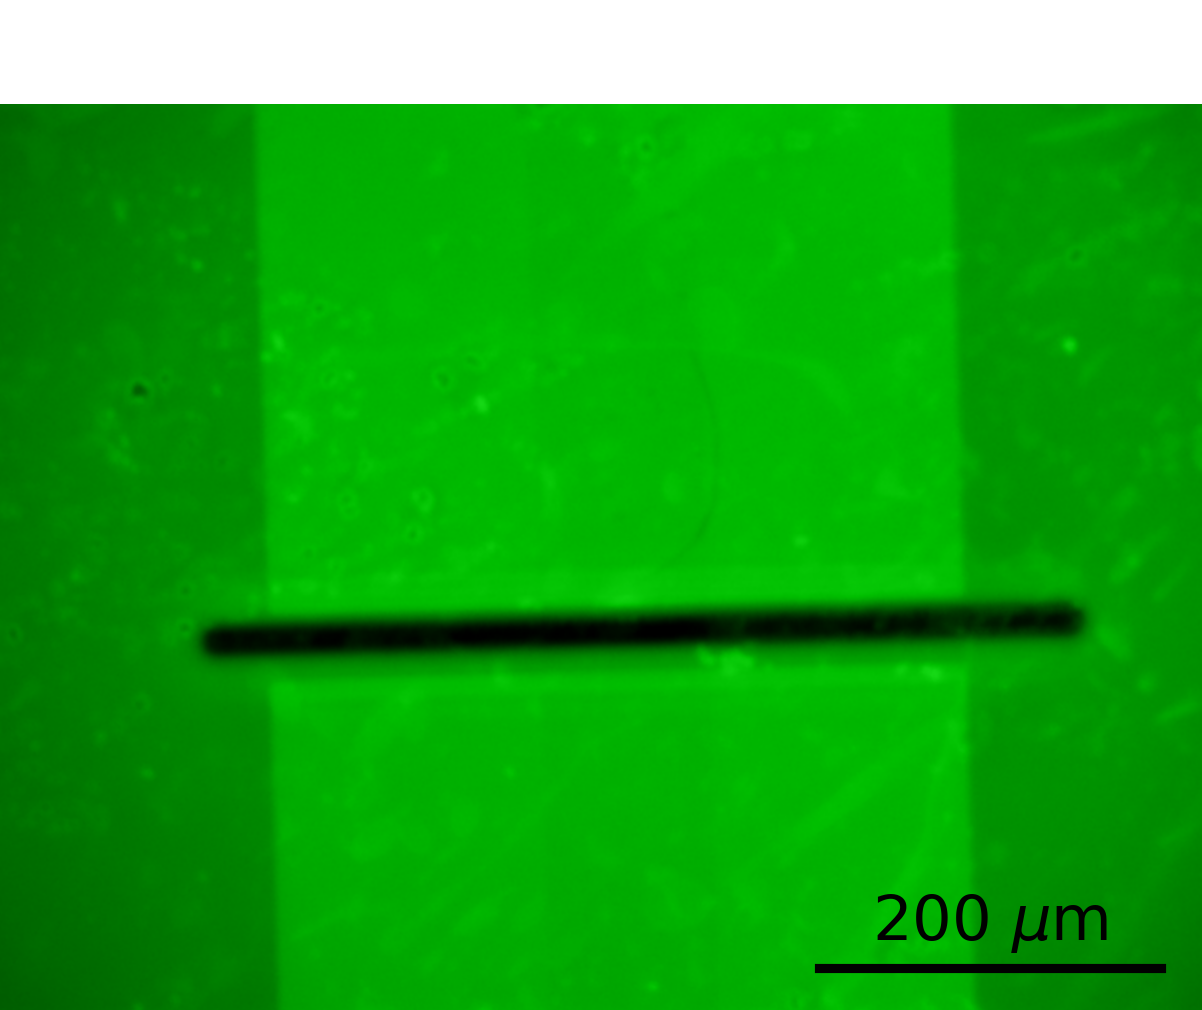
\includegraphics{figures/ch6/modified_CNT20_1mMPPF_channel8_350ms_12.6X_221124.png}

}

}

\end{minipage}%
%
\begin{minipage}[t]{0.01\linewidth}

{\centering 

~

}

\end{minipage}%
\newline
\begin{minipage}[t]{0.03\linewidth}

{\centering 

\raisebox{-\height}{


\includegraphics{figures/(c).png}

}

}

\end{minipage}%
%
\begin{minipage}[t]{0.01\linewidth}

{\centering 

~

}

\end{minipage}%
%
\begin{minipage}[t]{0.45\linewidth}

{\centering 

\raisebox{-\height}{

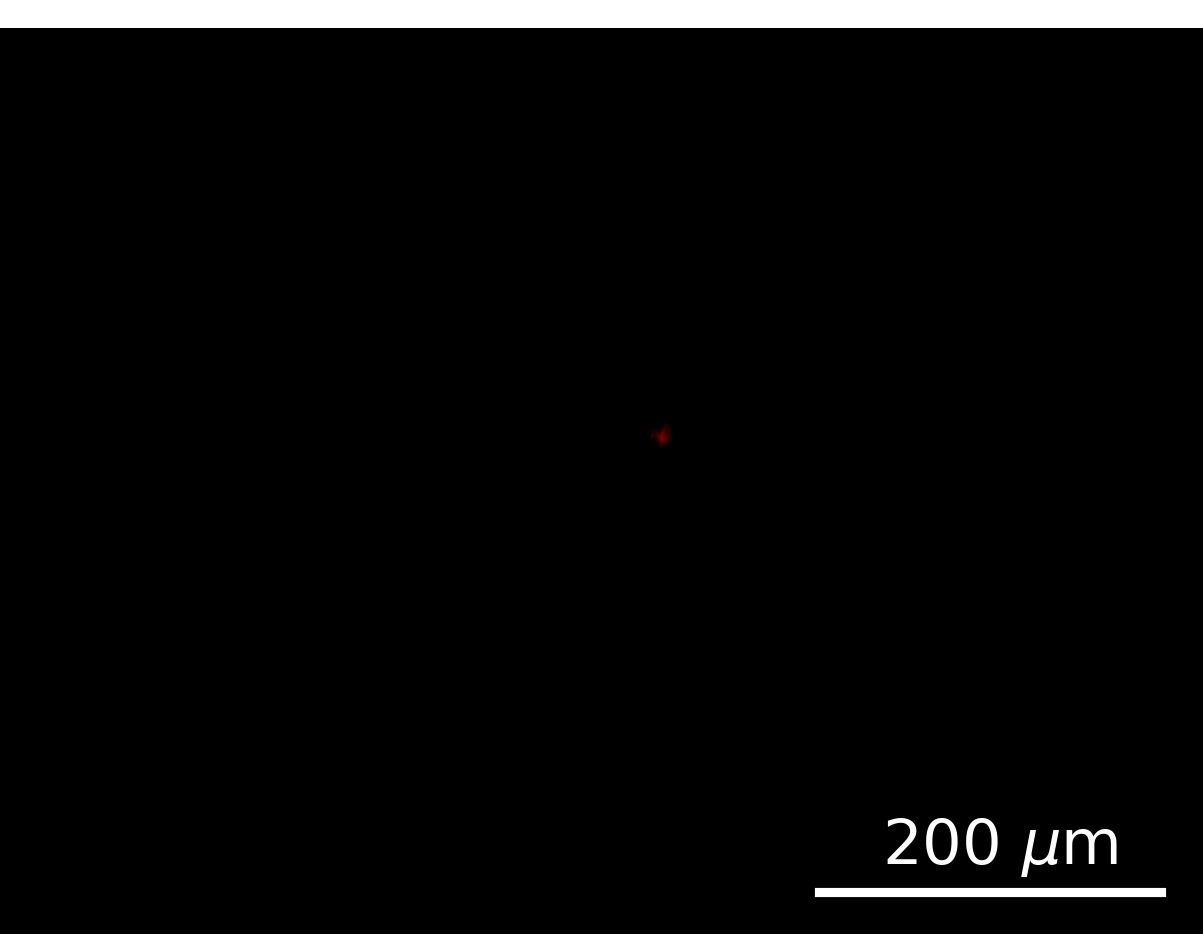
\includegraphics{figures/ch6/modified_Ccontrol_ch2_mCherry_10sexposure_highcontrast_12.6X.png}

}

}

\end{minipage}%
%
\begin{minipage}[t]{0.01\linewidth}

{\centering 

~

}

\end{minipage}%
%
\begin{minipage}[t]{0.03\linewidth}

{\centering 

\raisebox{-\height}{


\includegraphics{figures/(d).png}

}

}

\end{minipage}%
%
\begin{minipage}[t]{0.01\linewidth}

{\centering 

~

}

\end{minipage}%
%
\begin{minipage}[t]{0.45\linewidth}

{\centering 

\raisebox{-\height}{

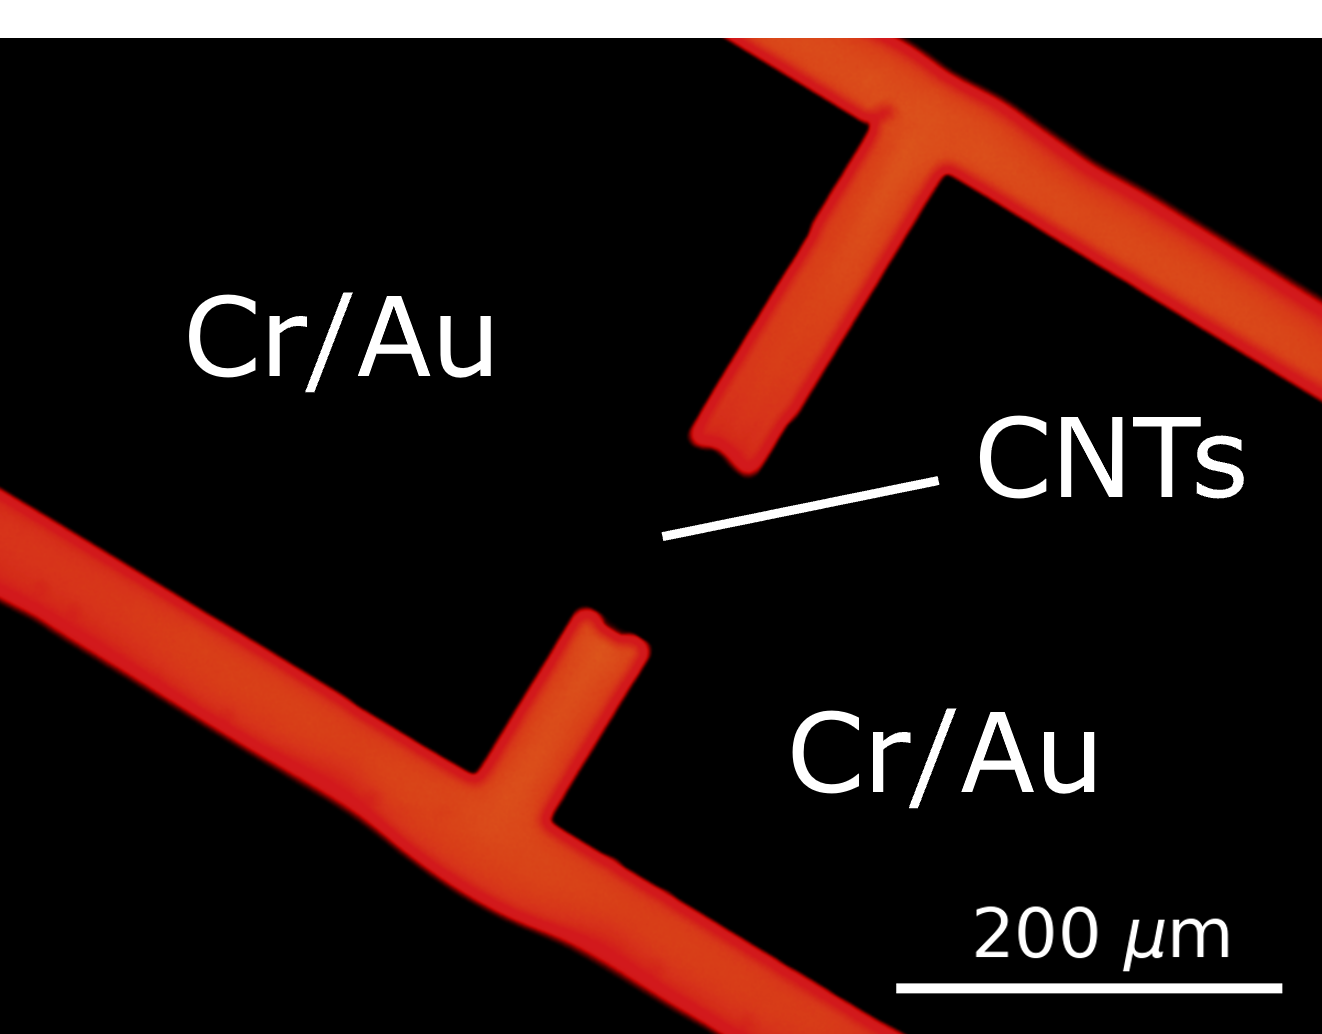
\includegraphics{figures/ch6/modified_C1_ch5_mCherry_10sexposure_highcontrast_12.6X.png}

}

}

\end{minipage}%
%
\begin{minipage}[t]{0.01\linewidth}

{\centering 

~

}

\end{minipage}%
\newline
\begin{minipage}[t]{0.03\linewidth}

{\centering 

\raisebox{-\height}{


\includegraphics{figures/(e).png}

}

}

\end{minipage}%
%
\begin{minipage}[t]{0.01\linewidth}

{\centering 

~

}

\end{minipage}%
%
\begin{minipage}[t]{0.45\linewidth}

{\centering 

\raisebox{-\height}{

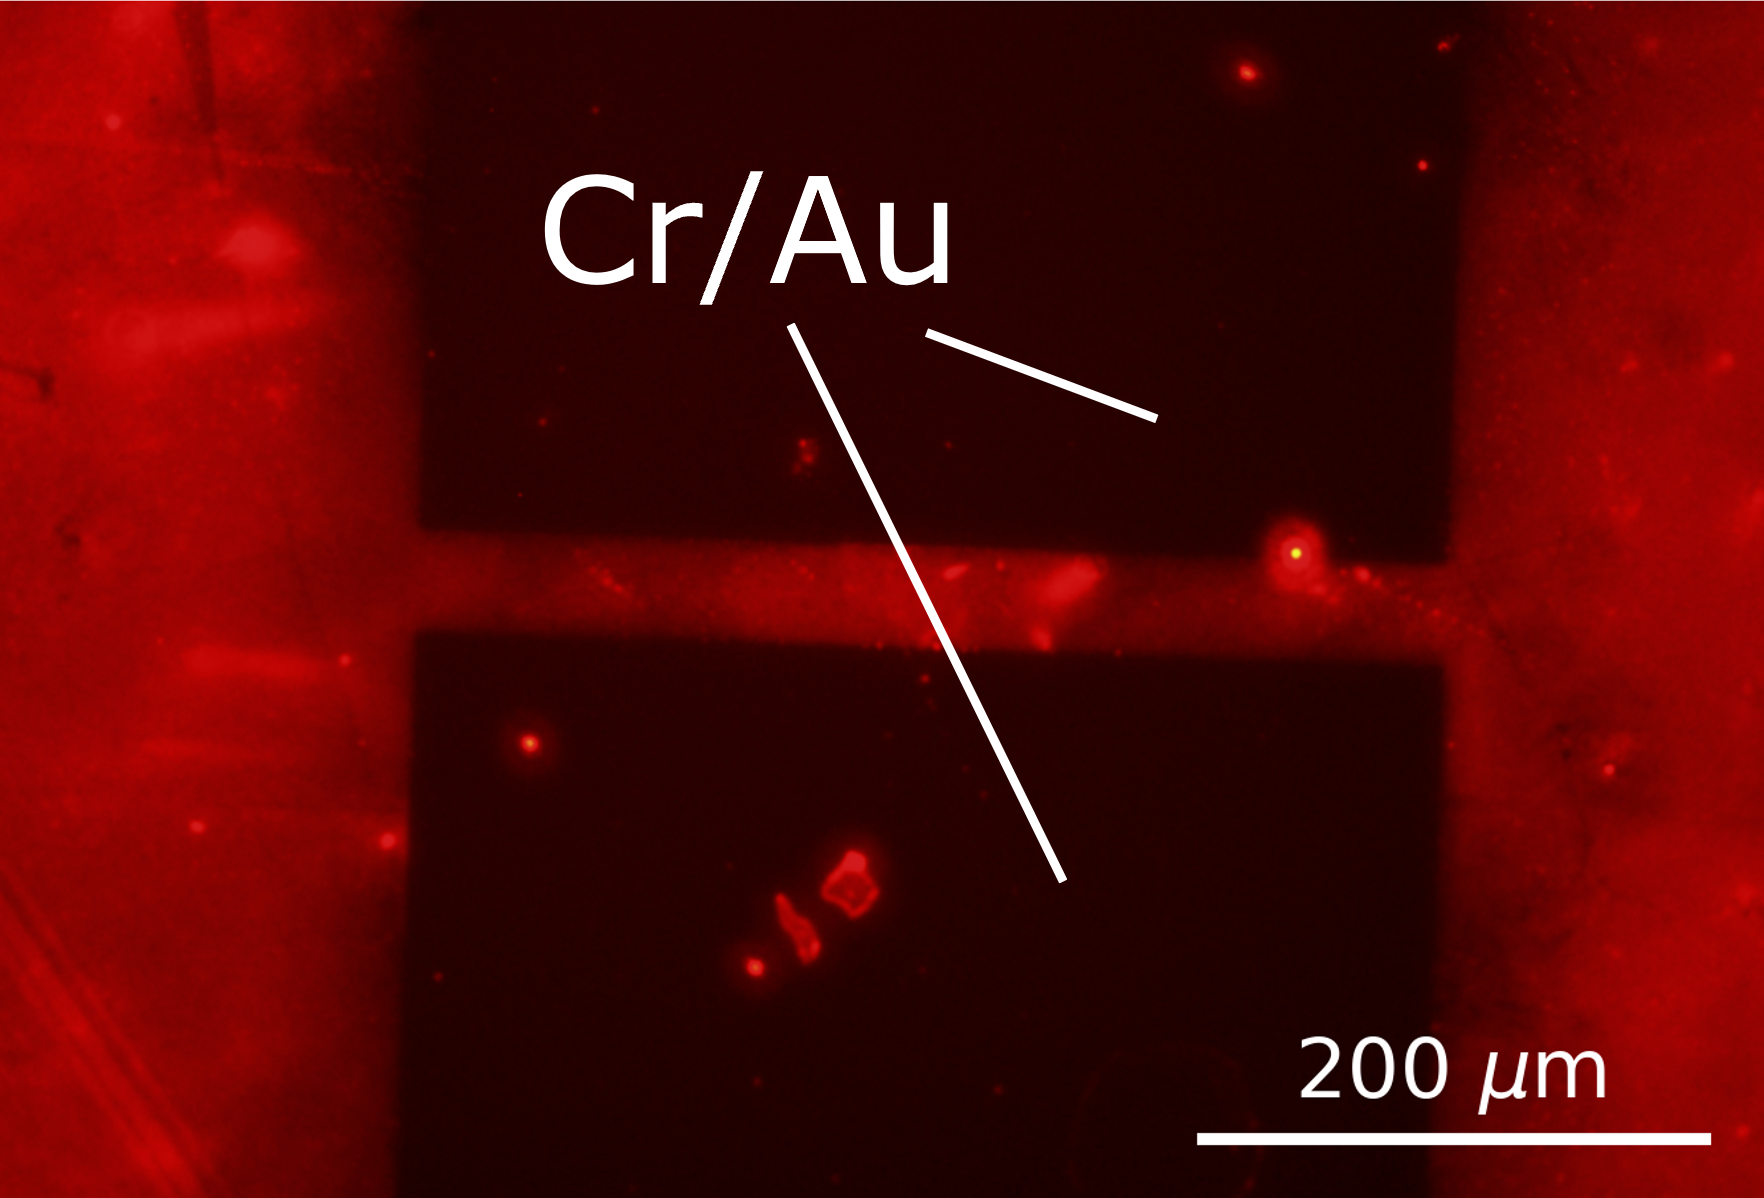
\includegraphics{figures/ch6/modified_softbake1minacetonerinse_aptamer_ch3_mCherry_30sexposure_highcontrast_ISO200_12.6X.png}

}

}

\end{minipage}%
%
\begin{minipage}[t]{0.01\linewidth}

{\centering 

~

}

\end{minipage}%
%
\begin{minipage}[t]{0.03\linewidth}

{\centering 

\raisebox{-\height}{


\includegraphics{figures/(f).png}

}

}

\end{minipage}%
%
\begin{minipage}[t]{0.01\linewidth}

{\centering 

~

}

\end{minipage}%
%
\begin{minipage}[t]{0.45\linewidth}

{\centering 

\raisebox{-\height}{

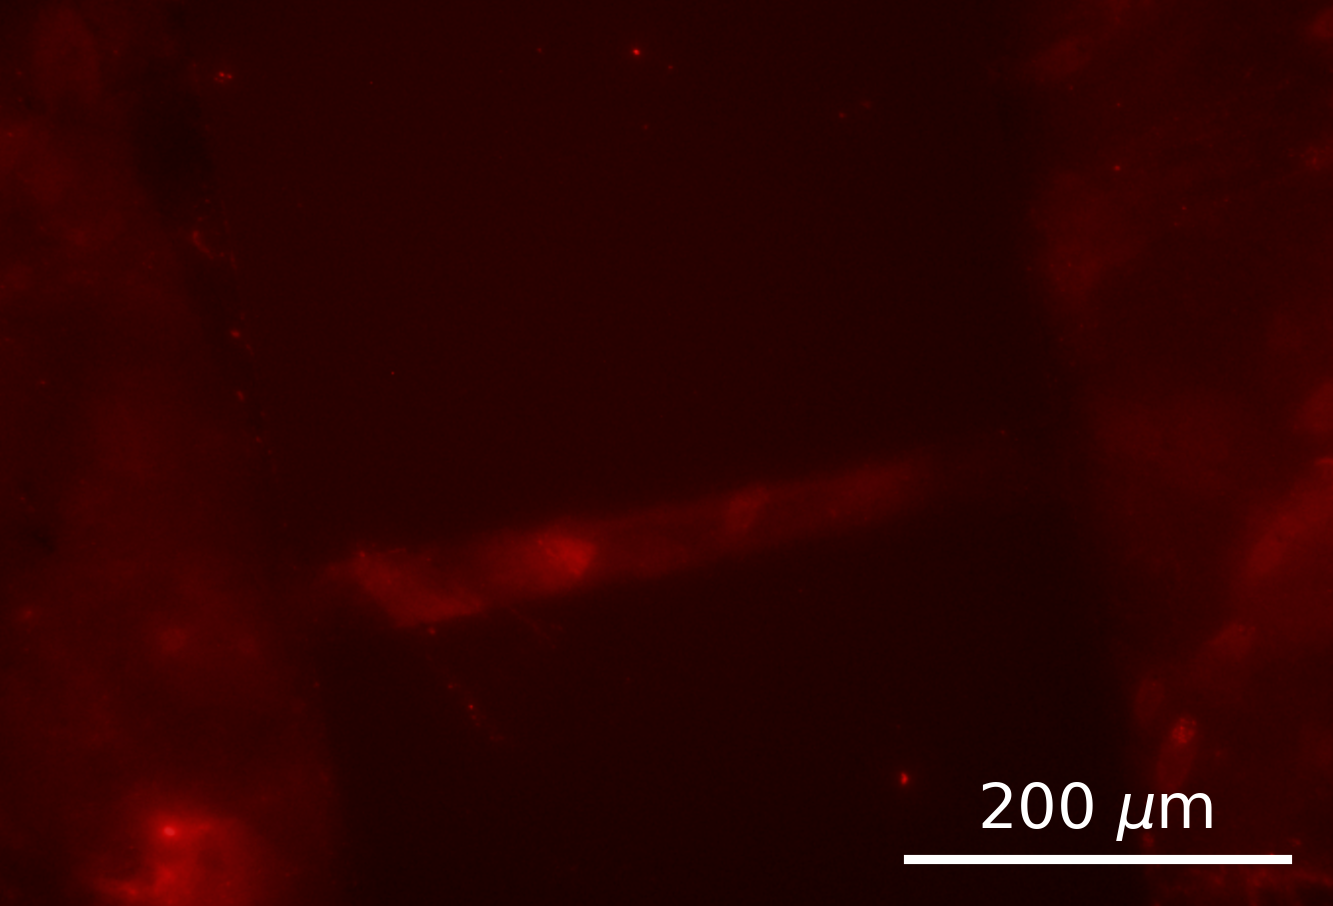
\includegraphics{figures/ch6/modified_hardbake_aptamer_ch3_mCherry_30sexposure_highcontrast_ISO200_12.6X.png}

}

}

\end{minipage}%
%
\begin{minipage}[t]{0.01\linewidth}

{\centering 

~

}

\end{minipage}%

\caption{\label{fig-photoresist-contamination}A fluorescence image of a
SU8-encapsulated carbon nanotube device is shown in (a), while (b) shows
the same channel after modification with an solution of 1 mM
Pyrene-PEG-FITC. A 0.35 s exposure time and FITC filter were used for
(a)-(b). The fluorescence image in (c) shows an unencapsulated channel,
while (d) shows the same channel after Cy3-tagged aptamer exposure. A 10
s exposure time and mCherry filter were used for (c)-(d). The
fluorescence images in (e) and (f) show devices pre-coated with a thin
layer of photoresist then submerged in Cy3-tagged aptamer, where the
device in (f) was hardbaked before aptamer exposure. An mCherry filter
and 30 s exposure time were used for for (e)-(f).}

\end{figure}

A similar interaction was seen between AZ\(^\circledR\) 1518 photoresist
and fluorescent-tagged, amine-terminated aptamer. An unencapsulated
carbon nanotube network device, fabricated using the pre-Jun 2022
process outlined in \textbf{?@sec-fabrication}, was incubated with 500
nM Cy3-tagged aptamer in Tris solution at 4°C overnight. The aptamer was
first denatured by heating in a water bath at 95°C for 5 minutes then
cooling in an ice bath for 10 minutes before use.
Figure~\ref{fig-photoresist-contamination} (c) and
Figure~\ref{fig-photoresist-contamination} (d) are fluorescence images
of the device channel region before and after exposure to aptamer. A
thick red ring is visible around the electrodes after functionalisation,
despite no PBASE being used to tether the amine-terminated aptamer. It
appears that these bright patches correspond to patches of residual
photoresist which have not been completely removed from the carbon
nanotube square by the development process. These patches have then
interacted with the aptamer, causing them to appear bright under the
fluorescence microscope. Beyond potentially interfering with
functionalisation, photoresist residue blocking a device channel will
prevent interaction with the Tris solution and prevent sensing.

To test whether residual resist could be prevented from interacting with
aptamer by crosslinking the resist, two unencapsulated devices were
prepared as follows. Devices were first spincoated with AZ\(^\circledR\)
1518 in the manner described in \textbf{?@sec-fabrication}. Next, the
majority of resist was removed by soaking the device in acetone for 1
minute. This process left a thin coating of photoresist on the devices.
One of these devices was then hardbaked at 200°C for 1 hour. Both
devices were subsequently functionalised in the following manner:

\begin{enumerate}
\def\labelenumi{\arabic{enumi}.}
\item
  Unencapsulated device was submerged in 1 mM PBASE in methanol solution
  for 1 hour.
\item
  The device was then rinsed with methanol and Tris.
\item
  1 µM Cy3-tagged aptamer was denatured by heating in a water bath at
  95°C for 5 minutes then cooling in an ice bath for 10 minutes before
  use.
\item
  The device was incubated with aptamer in Tris at 4°C overnight.
\end{enumerate}

Fluorescence microscope images of channels from each device are shown in
Figure~\ref{fig-photoresist-contamination} (e) and
Figure~\ref{fig-photoresist-contamination} (f), where the latter is the
device hardbaked before functionalisation. By comparing the two images,
it is apparent that hardbaking the AZ\(^\circledR\) 1518 photoresist
significantly reduces the amount of fluorescent aptamer attached to the
surface. This result is an indication that sufficient heating of the
photoresist can prevent it interacting with PBASE or amine-tagged
biological material. However, there is still some Cy3-tagged aptamer
fluorescence visible in Figure~\ref{fig-photoresist-contamination} (f).
It appears that hardbaking has not completely prevented photoresist from
interacting with the aptamer. It is possible that heating from the
bottom of the device is insufficient to hardbake the photoresist layer
completely, an effect that would be amplified for the thick photoresist
layer on encapsulated devices. Therefore, from Jun 2023 onwards devices
were vacuum annealed for 1 hour at 150°C prior to functionalisation.
This approach was taken to ensure photoresist was heated from above as
well as below and made chemically inert across its surface.

This result demonstrates the use of fluorescence microscopy as a tool to
detect residue and test suitable residue elimination measures. Further
testing showed that performing a 1 minute flood exposure (for positive
resist only) then placing a device in AZ\(^\circledR\) 326 developer for
3 minutes was highly effective at removing photoresist residue. Both
these development and annealing techniques were used for all
functionalised devices in subsequent sections.

\hypertarget{sec-hydrophobicity}{%
\subsection{Hydrophobicity of Carbon Nanotubes and
Graphene}\label{sec-hydrophobicity}}

\begin{figure}

\begin{minipage}[t]{0.03\linewidth}

{\centering 

\raisebox{-\height}{


\includegraphics{figures/(a).png}

}

}

\end{minipage}%
%
\begin{minipage}[t]{0.01\linewidth}

{\centering 

~

}

\end{minipage}%
%
\begin{minipage}[t]{0.45\linewidth}

{\centering 

\raisebox{-\height}{

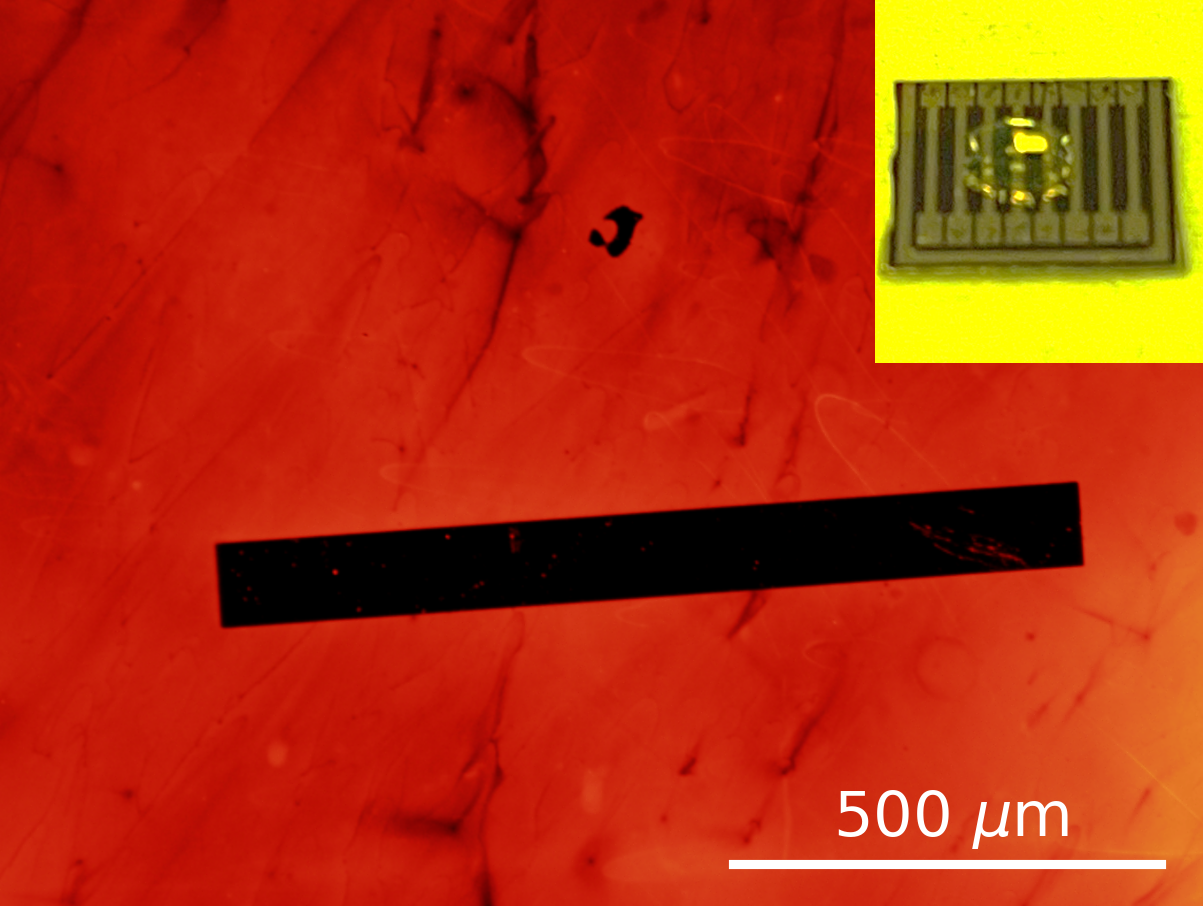
\includegraphics{figures/ch6/modified_NGW8D9_edgechannel_post10min50Cacetonerinse_221109.png}

}

}

\end{minipage}%
%
\begin{minipage}[t]{0.01\linewidth}

{\centering 

~

}

\end{minipage}%
%
\begin{minipage}[t]{0.03\linewidth}

{\centering 

\raisebox{-\height}{


\includegraphics{figures/(b).png}

}

}

\end{minipage}%
%
\begin{minipage}[t]{0.01\linewidth}

{\centering 

~

}

\end{minipage}%
%
\begin{minipage}[t]{0.45\linewidth}

{\centering 

\raisebox{-\height}{

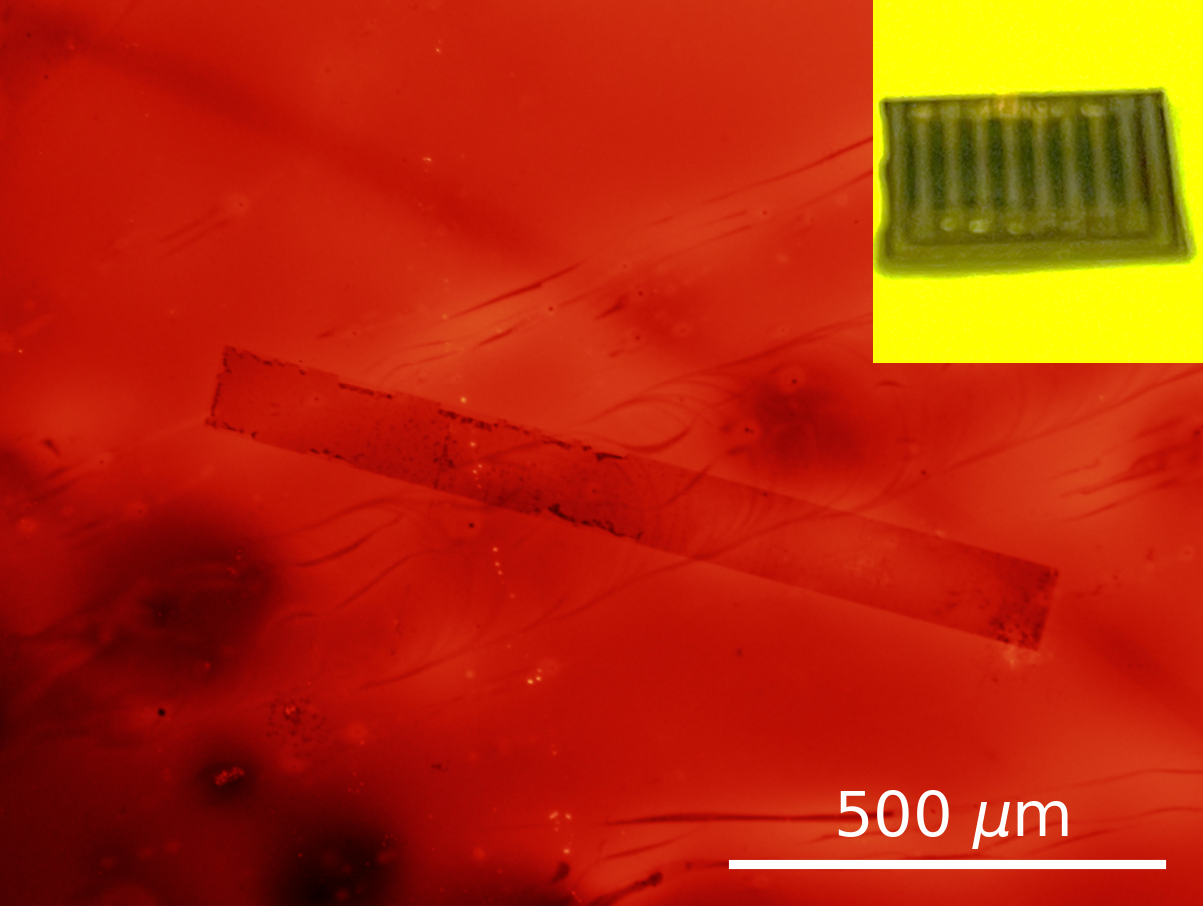
\includegraphics{figures/ch6/modified_NGW8D7_edgechannel_lowerexposuretime_221108.png}

}

}

\end{minipage}%
%
\begin{minipage}[t]{0.01\linewidth}

{\centering 

~

}

\end{minipage}%
\newline
\begin{minipage}[t]{0.03\linewidth}

{\centering 

\raisebox{-\height}{


\includegraphics{figures/(c).png}

}

}

\end{minipage}%
%
\begin{minipage}[t]{0.01\linewidth}

{\centering 

~

}

\end{minipage}%
%
\begin{minipage}[t]{0.45\linewidth}

{\centering 

\raisebox{-\height}{

\includegraphics{figures/ch6/modified_SiO2_1mMPPR_2_221109.png}

}

}

\end{minipage}%
%
\begin{minipage}[t]{0.01\linewidth}

{\centering 

~

}

\end{minipage}%
%
\begin{minipage}[t]{0.03\linewidth}

{\centering 

\raisebox{-\height}{

\includegraphics{figures/(d).png}

}

}

\end{minipage}%
%
\begin{minipage}[t]{0.01\linewidth}

{\centering 

~

}

\end{minipage}%
%
\begin{minipage}[t]{0.45\linewidth}

{\centering 

\raisebox{-\height}{

\includegraphics{figures/ch6/modified_NGW6D4_PyPEGFITC_channel2_1.6sexposure_10X_221122.png}

}

}

\end{minipage}%
%
\begin{minipage}[t]{0.01\linewidth}

{\centering 

~

}

\end{minipage}%
\newline
\begin{minipage}[t]{0.03\linewidth}

{\centering 

\raisebox{-\height}{

\includegraphics{figures/(e).png}

}

}

\end{minipage}%
%
\begin{minipage}[t]{0.01\linewidth}

{\centering 

~

}

\end{minipage}%
%
\begin{minipage}[t]{0.45\linewidth}

{\centering 

\raisebox{-\height}{

\includegraphics{figures/ch6/modified_NGW6D7_PyPEGFITC_channel3top_postmsurfclean_7.5sexposure_20X_221123.png}

}

}

\end{minipage}%
%
\begin{minipage}[t]{0.01\linewidth}

{\centering 

~

}

\end{minipage}%
%
\begin{minipage}[t]{0.03\linewidth}

{\centering 

\raisebox{-\height}{

\includegraphics{figures/(f).png}

}

}

\end{minipage}%
%
\begin{minipage}[t]{0.01\linewidth}

{\centering 

~

}

\end{minipage}%
%
\begin{minipage}[t]{0.45\linewidth}

{\centering 

\raisebox{-\height}{

\includegraphics{figures/ch6/modified_NGW6D7_PyPEGFITC_channel1_postmsurfclean_7.75sexposure_40X_221123.png}

}

}

\end{minipage}%
%
\begin{minipage}[t]{0.01\linewidth}

{\centering 

~

}

\end{minipage}%

\caption{\label{fig-silicon-dioxide-interaction}Fluorescence images of a
1000 µm \(\times\) 100 µm graphene channel. (a) was not oxygen plasma
cleaned before functionalisation with pyrene-PEG-rhodamine (PPR), while
(b) was oxygen plasma cleaned immediately before PPR functionalisation.
Insets show a water droplet on an unencapsulated device before (a) and
after (b) the being treated with O\(_2\) plasma. (c) shows a pristine
SiO\(_2\) surface after PPR exposure. (a), (b) and (c) were taken using
a Texas Red filter and a 1.8 s exposure time. (d) was functionalised
with 1 mM PPF in PBS after oxygen plasma treatment. (e) and (f) were
functionalised with 1 mM PPF after oxygen plasma treatment, then cleaned
with surfactant (m-CNT surfactant, NanoIntegris). (d), (e) and (f) were
taken using an FITC filter, with 1.6 s, 7.5 s and 7.75 s exposure times
respectively.}

\end{figure}

As PEGlyated linker dissolves well in aqueous solution, initial
fluorescence imaging focused on functionalising devices with these
linkers dissolved in \(1 \times\) PBS. It was hoped that by keeping the
device channels in a pH-controlled environment, the channel surface
would be made more suitable for the attached receptors.
Figure~\ref{fig-silicon-dioxide-interaction} (a) shows a graphene film
after exposure to pyrene-PEG-rhodamine (PPR) in \(1 \times\) PBS
solution for 1 hour. The pyrene-PEG-rhodamine has interacted with the
SiO\(_2\) substrate (discussed further in
Section~\ref{sec-pyrene-interactions}) but not the graphene film. The
graphene has not attached to the pyrene or rhodamine due to the highly
hydrophobic graphene surface repelling the surrounding solution,
preventing \(\pi\)-stacking from occurring. The hydrophobicity of the
graphene surface is not intrinsic to graphene. Instead, it results from
a hydrocarbon layer which forms on the channel surface when exposed to
air, primarily composed of long-chain alkanes
\autocite{Ashraf2014,Palinkas2022}. A hydrophobic layer wiil also form
on carbon nanotube networks \autocite{Stando2019,Park2022}. Treatment
with oxygen plasma at 5 W for 15 s has previously been found to remove
this hydrocarbon layer, restoring the intrinsic hydrophilicity of
graphene \autocite{Shin2010}. Storing the graphene surface in deionised
water rather than air prevents the return of this hydrocarbon layer
\autocite{Ashraf2014}. The use of a relatively low power plasma ensures
damage to the graphene layer is minimised.

Treatment of an unencapsulated carbon nanotube network device at 5 W for
15 s at 300 mTorr greatly reduced the contact angle of a water droplet
placed on the device surface. The water droplet before and after plasma
treatment is shown inset in Figure~\ref{fig-silicon-dioxide-interaction}
(a) and Figure~\ref{fig-silicon-dioxide-interaction} (b) respectively. A
graphene film was then functionalised with pyrene-PEG-rhodamine in
\(1 \times\) PBS in the same manner as for the film in
Figure~\ref{fig-silicon-dioxide-interaction} (a), except with the same
plasma treatment performed on the film less than 1 minute before
functionalisation. The result is shown in
Figure~\ref{fig-silicon-dioxide-interaction} (b). The graphene now
appears to interact with the pyrene-PEG-rhodamine. These results both
indicate that the plasma treatment is increasing the hydrophilicity of
the device surface, improving the ability of pyrene-PEG-rhodamine to
\(\pi\)-stack with graphene. The disadvantage of this procedure is that
the plasma cleaning introduces defects to the graphene surface which may
be undesirable for device electrical behaviour. Furthermore, it was
often found that devices functionalised in this manner had their
conductance drop significantly after functionalisation, even though
plasma treatment itself did not significantly alter device conductance.
Solvent was therefore used for the initial linker functionalisation in
\textbf{?@sec-biosensing-iORs}, as a plasma cleaning step was not
required for linker attachment.

\hypertarget{sec-pyrene-interactions}{%
\subsection{Substrate Interaction with Linker
Molecules}\label{sec-pyrene-interactions}}

Another issue that arose when verifying surface functionalisation was
the interaction between pyrene linker and the SiO\(_2\) substrate. This
interaction meant it was difficult to discern whether the pyrene group
was interacting in a specific manner with the channel film. It was
confirmed that pyrene-PEG was interacting with SiO\(_2\), rather than
residual photoresist or nanomaterial, by performing a
pyrene-PEG-rhodamine functionalisation on pristine SiO\(_2\), as shown
in Figure~\ref{fig-silicon-dioxide-interaction} (c). The PEGlyated
linker supplier suggested that the surface should be thoroughly rinsed
with surfactant to remove weakly-bound pyrene-PEG-FITC attached to the
SiO\(_2\), while preserving the pyrene-PEG-FITC strongly attached via
\(\pi\)-stacking to the graphene or carbon nanotube film
\autocite{CreativePEGworks2022}. The following process was then used to
remove pyrene-PEG-FITC from the SiO\(_2\): the film was rinsed with DI
water for 30 s, then placed in m-CNT dispersion solution (NanoIntegris)
for 5 minutes at 70°C while agitating with a pipette, and finally rinsed
with DI water, ethanol, acetone, IPA and nitrogen dried. A the graphene
region before cleaning is shown in
Figure~\ref{fig-silicon-dioxide-interaction} (d), while the results of
cleaning are shown in Figure~\ref{fig-silicon-dioxide-interaction} (e)
and Figure~\ref{fig-silicon-dioxide-interaction} (f). The majority of
pyrene-PEG-FITC was removed in regions with no graphene, but remained
where graphene was present, indicating specific, \(\pi\)-stacking
interaction took place between the pyrene-PEG-FITC and graphene.
However, this surfactant rinse step was not used when performing
functionalisation with biological materials, to prevent damage to the
lipid membranes used.

\hypertarget{sec-coffee-ring}{%
\subsection{Coffee-Ring Effect}\label{sec-coffee-ring}}

\begin{figure}

\begin{minipage}[t]{0.03\linewidth}

{\centering 

\raisebox{-\height}{

\includegraphics{figures/(a).png}

}

}

\end{minipage}%
%
\begin{minipage}[t]{0.01\linewidth}

{\centering 

~

}

\end{minipage}%
%
\begin{minipage}[t]{0.45\linewidth}

{\centering 

\raisebox{-\height}{

\includegraphics{figures/ch6/modified_GFPNi2+1_5sexposure_12.6X_mediumcontrast_18_230324.png}

}

}

\end{minipage}%
%
\begin{minipage}[t]{0.01\linewidth}

{\centering 

~

}

\end{minipage}%
%
\begin{minipage}[t]{0.03\linewidth}

{\centering 

\raisebox{-\height}{

\includegraphics{figures/(b).png}

}

}

\end{minipage}%
%
\begin{minipage}[t]{0.01\linewidth}

{\centering 

~

}

\end{minipage}%
%
\begin{minipage}[t]{0.45\linewidth}

{\centering 

\raisebox{-\height}{

\includegraphics{figures/ch6/modified_GFPNi2+1_5sexposure_12.6X_mediumcontrast_20_230324.png}

}

}

\end{minipage}%
%
\begin{minipage}[t]{0.01\linewidth}

{\centering 

~

}

\end{minipage}%

\caption{\label{fig-GFP-coffee-ring}Both (a) and (b) show a build-up of
his-tag GFP at the edges of the droplet region where pyrene-PEG-NTA had
been present, taken using an GFP filter and a 5 s exposure time. On the
right hand side of (b), no his-tag GFP is visible on the metal
electrode, as no pyrene-PEG attaches to the metal electrodes.}

\end{figure}

From Table~\ref{tbl-pbase-functionalisation}, full device submersion
appears to be the most common approach for functionalisation with
solution containing linker molecules like PBASE. However, some groups
placed small droplets of solution onto the device channels when
functionalisation, and this approach was tested as part of the
fluorescence verification work. For functionalisation with his-tagged
green fluorescent protein, after plasma cleaning at 5 W for 15 s at 300
mTorr, a 4 µL droplet of 100 µM pyrene-PEG-NTA in \(1 \times\) PBS was
placed on each graphene device channel and left covered in a humid
environment for 15 minutes. The device was then rinsed with \(1 \times\)
PBS, submerged in 10 mM NiSO\(_4\) in \(1 \times\) PBS for 1 hour,
rinsed in \(1 \times\) PBS, then submerged in 10 mL of 100 ng/mL his-tag
GFP solution (Thermofisher) overnight. Fluorescence microscope imaging
showed that a ring of biomaterial would build up around the outer edge
of regions where pyrene-PEG-NTA had been present, as seen in
Figure~\ref{fig-GFP-coffee-ring}.

It appears this non-specific binding is a result of the his-tag GFP
attaching to a dense region of pyrene-PEG-NTA at the edge of the
functionalisation droplet. This accretion of pyrene-PEG-NTA at the edge
of the droplet is a result of the coffee-ring effect, where the
evaporation of the droplet leads to transport of particles to the
droplet edges via capillary flow \autocite{Deegan1997,Shimobayashi2018}.
As this gradient in surface coverage of attached proteins has unknown
consequences for sensing, in the subsequent chapter devices were always
functionalised by submerging them in solution instead of dropcasting.

\hypertarget{sec-conclusion}{%
\section{Conclusion}\label{sec-conclusion}}

It has been well-established in the literature that the \(\pi\)-stacking
reaction mechanism between pyrene-based linkers and graphene and carbon
nanotube network field-effect transistors can be used to create working
biosensors. The previous use of various linker molecules for biosensor
functionalisation was investigated. Despite the wide use of
1-pyrenebutanoic acid N-hydroxysuccinimide ester (PBASE) and
1-pyrenebutyric acid (PBA) for functionalisation of biosensors, the
literature shows a significant variation in the methods used for
attachment of linker molecules to a transistor channel. The most common
methods, using 6 mM PBASE dissolved in dimethylformamide or 1 mM PBASE
in methanol, stem directly from the first documented use of PBASE for
functionalisation of carbon nanotube biosensors. In the last 6 years,
more research has been done into optimising the PBASE methodology for
graphene devices, but there is still disagreement in the literature over
whether minimising or maximising PBASE coverage on a graphene device
channel is desirable for sensing. Due to disagreement in the literature
around suitable non-covalent methods for biosensor functionalisation,
several steps were taken to identify a rapid and simple method for
verifying successful functionalisation, and to locate any potential
barriers to a successful functionalisation.

The advantages and disadvantages of these linker molecules were first
compared. Hydrogen NMR indicated that water was present in PBASE samples
prepared in DMSO. The potential for PBASE to hydrolyse during
functionalisation means that the presence of water is strongly
undesirable. The reaction of PBA with EDC in the presence of NHS is an
alternative functionalisation approach which is less prone to
hydrolysis. However, this process has its own disadvantages, such as
undesirable protein interactions and the increased amount of steps and
process variables involved. Pyrene-NTA is also less prone to hydrolysis
than PBASE, but unlike PBASE or PBA/EDC, interacts with a specific
protein tag (his-tag). PEGlyation of the pyrene-NTA linker also means
that the entire functionalisation process can be performed in aqueous
solution, avoiding the introduction of non-organic solvents. This
approach is desirable, since the non-aqueous solvents traditionally used
for functionalisation may have negative impacts on device behaviour. For
example, carbon nanotube device channel transfer characteristics were
found to undergo a significant shift of \(\Delta V = -0.15 \pm 0.02\)
when exposed to DMSO or MeOH for 1 hour.

Next, it was verified that the pyrene groups of the linker molecules of
interest were attaching successfully to either carbon nanotubes or
graphene. Raman spectroscopy showed that incubating a highly-bundled
carbon nanotube film in 5 mM PBASE or PBA in DMSO for 1 hour increased
\(I_D/I_G\) by a factor of \(\sim 3\) relative to the DMSO-only case.
Incubating a steam-deposited carbon nanotube device in a 1 mM
concentration of PBASE in methanol or DMSO for 1 hour was found to cause
a significant increase in device on-current relative to the solvent-only
case, and a similar increase in on-current was seen for 5 mM PBA in DMSO
relative to the DMSO-only case. When a PBA-functionalised device was
placed in aqueous solution with 20 mM EDC and 40 mM NHS for 30 minutes,
a further increase in on-current was seen. Fluorescence microscopy was
used to demonstrate the successful attachment of pyrene-PEG to graphene
using an attached FITC probe, where immersing a graphene film in 1 mM
pyrene-PEG in ethanol led to the channels becoming brightly fluorescent
relative to the background using a 1 s exposure time.

Various obstacles to successful functionalisation were also encountered
and addressed using fluorescence microscopy. Photoresist contamination
was addressed with exposure and development steps before
functionalisation, with the exposure skipped for negative-resist
encapsulated devices. Hydrophobicity of graphene films was addressed by
plasma treatment before functionalisation in aqueous solution. A
surfactant rinse was used to distinguish between weak substrate-linker
interaction and \(\pi\)-stacking between linker and the channel.
Finally, coffee-ring distribution of linker was addressed by always
fully submerging the device in linker when functionalising.

\cleardoublepage
\phantomsection
\addcontentsline{toc}{part}{Appendices}
\appendix

\hypertarget{vapour-system-hardware}{%
\chapter{Vapour System Hardware}\label{vapour-system-hardware}}

\hypertarget{tbl-vapour-sensor-components}{}
\begin{longtable}[]{@{}
  >{\raggedright\arraybackslash}p{(\columnwidth - 4\tabcolsep) * \real{0.5930}}
  >{\raggedright\arraybackslash}p{(\columnwidth - 4\tabcolsep) * \real{0.2209}}
  >{\raggedright\arraybackslash}p{(\columnwidth - 4\tabcolsep) * \real{0.1860}}@{}}
\caption{\label{tbl-vapour-sensor-components}Major components used in
construction of the vapour delivery system described in this
thesis.}\tabularnewline
\toprule\noalign{}
\begin{minipage}[b]{\linewidth}\raggedright
Description
\end{minipage} & \begin{minipage}[b]{\linewidth}\raggedright
Part No.
\end{minipage} & \begin{minipage}[b]{\linewidth}\raggedright
Manufacturer
\end{minipage} \\
\midrule\noalign{}
\endfirsthead
\toprule\noalign{}
\begin{minipage}[b]{\linewidth}\raggedright
Description
\end{minipage} & \begin{minipage}[b]{\linewidth}\raggedright
Part No.
\end{minipage} & \begin{minipage}[b]{\linewidth}\raggedright
Manufacturer
\end{minipage} \\
\midrule\noalign{}
\endhead
\bottomrule\noalign{}
\endlastfoot
Mass flow controller, 20 sccm full scale & GE50A-013201SBV020 & MKS
Instruments \\
Mass flow controller, 200 sccm full scale & GE50A-013202SBV020 & MKS
Instruments \\
Mass flow controller, 500 sccm full scale & FC-2901V & Tylan \\
Analogue flowmeter, 240 sccm max. flow & 116261-30 & Dwyer \\
Micro diaphragm pump & P200-B3C5V-35000 & Xavitech \\
Analogue flow controller, for micro diaphragm pump & X3000450 &
Xavitech \\
10 mL Schott bottle & 218010802 & Duran \\
PTFE connection cap system & Z742273 & Duran \\
Baseline VOC-TRAQ flow cell, purple & 043-950 & Ametek Mocon \\
Baseline VOC-TRAQ flow cell, red & 043-951 & Ametek Mocon \\
Humidity and temperature sensor & T9602-5-A & Telaire \\
\end{longtable}

\hypertarget{python-code-for-data-analysis}{%
\chapter{Python Code for Data
Analysis}\label{python-code-for-data-analysis}}

\hypertarget{code-repository}{%
\section{Code Repository}\label{code-repository}}

The code used for general analysis of field-effect transistor devices in
this thesis was written with Python 3.8.8. Contributors to the code used
include Erica Cassie, Erica Happe, Marissa Dierkes and Leo Browning. The
code is located on GitHub and the research group OneDrive, and is
available on request.

\hypertarget{sec-histogram-analysis}{%
\section{Atomic Force Microscope Histogram
Analysis}\label{sec-histogram-analysis}}

The purpose of this code is to analyse atomic force microscope (AFM)
images of carbon nanotube networks in .xyz format taken using an atomic
force microscope and processed in Gwyddion (see
\textbf{?@sec-afm-characterisation}). It was originally designed by
Erica Happe in Matlab, and adapted by Marissa Dierkes and myself for use
in Python. The code imports the .xyz data and sorts it into bins 0.15 nm
in size for processing. To perform skew-normal distribution fits, both
\emph{scipy.optimize.curve\_fit} and \emph{scipy.stats.skewnorm} modules
are used in this code.

\hypertarget{sec-raman-analysis}{%
\section{Raman Spectroscopy Analysis}\label{sec-raman-analysis}}

The purpose of this code is to analyse a series of Raman spectra taken
at different points on a single film (see
\textbf{?@sec-raman-characterisation}). Data is imported in a series of
tab-delimited text files, with the low wavenumber spectrum (100
cm\(^{-1} - 650\) cm\(^{-1}\)) and high wavenumber spectrum (1300
cm\(^{-1} - 1650\) cm\(^{-1}\)) imported in separate datafiles for each
scan location.

\hypertarget{sec-field-effect-transistor-analysis}{%
\section{Field-Effect Transistor
Analysis}\label{sec-field-effect-transistor-analysis}}

The purpose of this code is to analyse electrical measurements taken of
field-effect transistor (FET) devices. Electrical measurements were
either taken from the Keysight 4156C Semiconductor Parameter Analyser,
National Instruments NI-PXIe or Keysight B1500A Semiconductor Device
Analyser as discussed in \textbf{?@sec-electrical-characterisation}; the
code is able to analyse data in .csv format taken from all three
measurement setups. The main Python file in the code base consists of
three related but independent modules: the first analyses and plots
sensing data from the FET devices, the second analyses and plots
transfer characteristics from channels across a device, and the third
compares individual channel characteristics before and after a
modification or after each individual modification in a series of
modifications. The code base also features a separate config file and
style sheet which govern the behaviour of the main code. The code base
was designed collaboratively by myself and Erica Cassie over GitHub
using the Sourcetree Git GUI.

\hypertarget{references}{%
\chapter*{References}\label{references}}
\addcontentsline{toc}{chapter}{References}

\markboth{References}{References}

\printbibliography[heading=none]


\backmatter

\end{document}
